% Options for packages loaded elsewhere
\PassOptionsToPackage{unicode}{hyperref}
\PassOptionsToPackage{hyphens}{url}
\PassOptionsToPackage{dvipsnames,svgnames,x11names}{xcolor}
\documentclass[
  10pt,
]{article}
\usepackage{xcolor}
\usepackage[margin=2.2cm]{geometry}
\usepackage{amsmath,amssymb}
\setcounter{secnumdepth}{-\maxdimen} % remove section numbering
\usepackage{iftex}
\ifPDFTeX
  \usepackage[T1]{fontenc}
  \usepackage[utf8]{inputenc}
  \usepackage{textcomp} % provide euro and other symbols
\else % if luatex or xetex
  \usepackage{unicode-math} % this also loads fontspec
  \defaultfontfeatures{Scale=MatchLowercase}
  \defaultfontfeatures[\rmfamily]{Ligatures=TeX,Scale=1}
\fi
\usepackage{lmodern}
\ifPDFTeX\else
  % xetex/luatex font selection
\fi
% Use upquote if available, for straight quotes in verbatim environments
\IfFileExists{upquote.sty}{\usepackage{upquote}}{}
\IfFileExists{microtype.sty}{% use microtype if available
  \usepackage[]{microtype}
  \UseMicrotypeSet[protrusion]{basicmath} % disable protrusion for tt fonts
}{}
\makeatletter
\@ifundefined{KOMAClassName}{% if non-KOMA class
  \IfFileExists{parskip.sty}{%
    \usepackage{parskip}
  }{% else
    \setlength{\parindent}{0pt}
    \setlength{\parskip}{6pt plus 2pt minus 1pt}}
}{% if KOMA class
  \KOMAoptions{parskip=half}}
\makeatother
\usepackage{color}
\usepackage{fancyvrb}
\newcommand{\VerbBar}{|}
\newcommand{\VERB}{\Verb[commandchars=\\\{\}]}
\DefineVerbatimEnvironment{Highlighting}{Verbatim}{commandchars=\\\{\}}
% Add ',fontsize=\small' for more characters per line
\newenvironment{Shaded}{}{}
\newcommand{\AlertTok}[1]{\textcolor[rgb]{1.00,0.00,0.00}{\textbf{#1}}}
\newcommand{\AnnotationTok}[1]{\textcolor[rgb]{0.38,0.63,0.69}{\textbf{\textit{#1}}}}
\newcommand{\AttributeTok}[1]{\textcolor[rgb]{0.49,0.56,0.16}{#1}}
\newcommand{\BaseNTok}[1]{\textcolor[rgb]{0.25,0.63,0.44}{#1}}
\newcommand{\BuiltInTok}[1]{\textcolor[rgb]{0.00,0.50,0.00}{#1}}
\newcommand{\CharTok}[1]{\textcolor[rgb]{0.25,0.44,0.63}{#1}}
\newcommand{\CommentTok}[1]{\textcolor[rgb]{0.38,0.63,0.69}{\textit{#1}}}
\newcommand{\CommentVarTok}[1]{\textcolor[rgb]{0.38,0.63,0.69}{\textbf{\textit{#1}}}}
\newcommand{\ConstantTok}[1]{\textcolor[rgb]{0.53,0.00,0.00}{#1}}
\newcommand{\ControlFlowTok}[1]{\textcolor[rgb]{0.00,0.44,0.13}{\textbf{#1}}}
\newcommand{\DataTypeTok}[1]{\textcolor[rgb]{0.56,0.13,0.00}{#1}}
\newcommand{\DecValTok}[1]{\textcolor[rgb]{0.25,0.63,0.44}{#1}}
\newcommand{\DocumentationTok}[1]{\textcolor[rgb]{0.73,0.13,0.13}{\textit{#1}}}
\newcommand{\ErrorTok}[1]{\textcolor[rgb]{1.00,0.00,0.00}{\textbf{#1}}}
\newcommand{\ExtensionTok}[1]{#1}
\newcommand{\FloatTok}[1]{\textcolor[rgb]{0.25,0.63,0.44}{#1}}
\newcommand{\FunctionTok}[1]{\textcolor[rgb]{0.02,0.16,0.49}{#1}}
\newcommand{\ImportTok}[1]{\textcolor[rgb]{0.00,0.50,0.00}{\textbf{#1}}}
\newcommand{\InformationTok}[1]{\textcolor[rgb]{0.38,0.63,0.69}{\textbf{\textit{#1}}}}
\newcommand{\KeywordTok}[1]{\textcolor[rgb]{0.00,0.44,0.13}{\textbf{#1}}}
\newcommand{\NormalTok}[1]{#1}
\newcommand{\OperatorTok}[1]{\textcolor[rgb]{0.40,0.40,0.40}{#1}}
\newcommand{\OtherTok}[1]{\textcolor[rgb]{0.00,0.44,0.13}{#1}}
\newcommand{\PreprocessorTok}[1]{\textcolor[rgb]{0.74,0.48,0.00}{#1}}
\newcommand{\RegionMarkerTok}[1]{#1}
\newcommand{\SpecialCharTok}[1]{\textcolor[rgb]{0.25,0.44,0.63}{#1}}
\newcommand{\SpecialStringTok}[1]{\textcolor[rgb]{0.73,0.40,0.53}{#1}}
\newcommand{\StringTok}[1]{\textcolor[rgb]{0.25,0.44,0.63}{#1}}
\newcommand{\VariableTok}[1]{\textcolor[rgb]{0.10,0.09,0.49}{#1}}
\newcommand{\VerbatimStringTok}[1]{\textcolor[rgb]{0.25,0.44,0.63}{#1}}
\newcommand{\WarningTok}[1]{\textcolor[rgb]{0.38,0.63,0.69}{\textbf{\textit{#1}}}}
\usepackage{longtable,booktabs,array}
\usepackage{caption}
\captionsetup[table]{skip=6pt}
\newcounter{none} % for unnumbered tables
\usepackage{calc} % for calculating minipage widths
% Correct order of tables after \paragraph or \subparagraph
\usepackage{etoolbox}
\makeatletter
\patchcmd\longtable{\par}{\if@noskipsec\mbox{}\fi\par}{}{}
\makeatother
\usepackage{graphicx}
\makeatletter
\newsavebox\pandoc@box
\newcommand*\pandocbounded[1]{% scales image to fit in text height/width
  \sbox\pandoc@box{#1}%
  \Gscale@div\@tempa{\textheight}{\dimexpr\ht\pandoc@box+\dp\pandoc@box\relax}%
  \Gscale@div\@tempb{\linewidth}{\wd\pandoc@box}%
  \ifdim\@tempb\p@<\@tempa\p@\let\@tempa\@tempb\fi% select the smaller of both
  \ifdim\@tempa\p@<\p@\scalebox{\@tempa}{\usebox\pandoc@box}%
  \else\usebox{\pandoc@box}%
  \fi%
}
% Set default figure placement to htbp
\def\fps@figure{htbp}
\makeatother
\ifLuaTeX
  \usepackage{luacolor}
  \usepackage[soul]{lua-ul}
\else
  \usepackage{soul}
\fi
\setlength{\emergencystretch}{3em} % prevent overfull lines
\providecommand{\tightlist}{%
  \setlength{\itemsep}{0pt}\setlength{\parskip}{0pt}}

\usepackage{booktabs}
\usepackage{longtable}
\usepackage{array}
\usepackage{etoolbox}
\usepackage{graphicx}
\usepackage{float}
\AtBeginEnvironment{longtable}{\footnotesize}
\setlength{\tabcolsep}{4pt}
\renewcommand{\arraystretch}{1.05}
\setlength{\emergencystretch}{2em}
% 图注编号由正文手写（"**Figure N.**"），这里关掉 LaTeX 的自动编号与分隔符，避免双编号
\captionsetup[figure]{labelformat=empty,labelsep=none}
\usepackage{bookmark}
\IfFileExists{xurl.sty}{\usepackage{xurl}}{} % add URL line breaks if available
\urlstyle{same}
% fallback for those not using the hyperref driver hyperxmp:
\makeatletter
\@ifundefined{xmpquote}{\newcommand{\xmpquote}[1]{#1}}{}
\makeatother
\hypersetup{
  pdftitle={Applicability Is Not Competitiveness: An Independent Evaluation and a Data-Side Repair for BQ-Native Graph Indexing},
  pdfauthor={AUTHOR NAMES, AFFILIATION, E-MAIL {[}TO BE FILLED IN BY THE AUTHORS{]}},
  colorlinks=true,
  linkcolor={Maroon},
  filecolor={Maroon},
  citecolor={Blue},
  urlcolor={Blue},
  pdfcreator={LaTeX via pandoc}}

\title{Applicability Is Not Competitiveness: An Independent Evaluation
and a Data-Side Repair for BQ-Native Graph Indexing}
\author{AUTHOR NAMES, AFFILIATION, E-MAIL {[}TO BE FILLED IN BY THE
AUTHORS{]}}
\date{October 9, 2026}

\begin{document}
\maketitle
\begin{abstract}
Binary-quantized graph indexes navigate on 2-bit codes instead of
full-precision vectors, and the published answer to ``when is that
usable?'' is a 12-dataset table spanning 0.40 \% $\rightarrow$ 95.65 \% Recall@10
plus a single index-free compatibility probe. We re-run that benchmark
on the authors' released implementation (11 of 12 rows reproduced within
$\pm$1.84 pp; one row is protocol-ambiguous) and report five things the
published account does not cover. (i) The table's tiers describe
applicability, and are read as competitiveness; where competitor curves
exist, three of the four tiers are dominated by plain HNSW --- on
several rows QuIVer's recall ceiling lies below the baseline's lowest
operating point, so the curves cannot intersect. (ii) The bottom tier
mixes three different failures: a repairable encoding failure (the sign
plane is globally constant, sign\_info = 0.000), an index-agnostic task
failure on which every competitor also collapses (Random-Sphere 1.40 \%,
Gaussian-960 1.10--1.39 \% across three HNSW implementations at ef=64),
and a capacity failure (coco\_nomic) where the bit budget, not the
distribution, is binding --- at 4 bits per dimension every collapse row
measures $\geq$ 94.6 \%. (iii) The published probe is under-specified --- it
does not fix the BQ distance, the sample size, or the instrument.
Implemented with the paper's own default distance, it calls
Random-Sphere compatible (53.9\%) on a dataset whose measured recall is
0.91 \%; taking the weaker of the engine's two distances removes this
false positive without changing any other verdict, and a sign-entropy
statistic paired with it yields a four-step decision chain validated on
22 arms. (iv) The collapse is repairable without touching the index: one
translation (x' = normalize(x $-$ $\mu$)) takes GIST-960 from 2.10 \% to 39.74
\% and SIFT-128 from 15.77 \% to 30.64 \% at ef=64, with an isotropic
control moving +0.03 pp; making the L0 navigation metric match the
metric the graph was built with adds up to +21.8 pp where the sign plane
is alive and hurts where it is dead, so we ship it as a default-off
switch with a decision rule. After the repair two arms move from
``dominated'' to ``parity'' or ``intersecting'' --- but the honest
sentence survives: a smaller gap is not availability. (v) The missing
baseline class (§5.6): an OPQ+IVF-PQ+Refine pipeline with the same f32
re-ranking never collapses on any of the six cells we measured ---
including the two where the 2-bit code collapses hardest --- at $\approx$ 4.7$\times$
QuIVer's memory, so the published boundary is the 2-bit code's, not
quantization's. We do not claim the paper is wrong (its mechanism is the
one we measure), we propose no new quantizer, and we report our own two
failed attempts at a single-scalar recall predictor.
\end{abstract}

{
\setcounter{tocdepth}{3}
\tableofcontents
}
\textbf{Evidence base.} Every number in this paper resolves to a file
under \texttt{results/**} or a log under \texttt{.tmp/}; the audit trail
--- including our own conclusions that were retracted along the way, and
the protocol correction of §5.6(b) --- is in
\texttt{docs/research/*.md}. The only library change is a default-off
switch shipped as \texttt{patches/f1-nav-weighted.patch}.

\section{1. Introduction}\label{introduction}

Binary-quantized (BQ) graph indexes promise a graph that navigates on
2-bit codes instead of full-precision vectors: an order of magnitude
less memory, and a hot path that is mostly popcount. Whether such an
index is \emph{usable} on a given embedding distribution is therefore a
question with real deployment consequences --- and it is the question
the QuIVer paper (PVLDB 20) answers with a cross-dataset table spanning
more than 90 points of Recall@10 (0.40 \% $\rightarrow$ 95.65 \%) and a single
index-free probe that predicts which side of the usability line a
dataset is on.

This paper is an independent evaluation of that claim, plus a
constructive repair of its two weakest points. We re-run the published
benchmark on the released implementation, on a machine without AVX-512,
and report what survives, what does not, and what a deployer should do
instead.

\textbf{What we find.}

\begin{enumerate}
\def\labelenumi{\arabic{enumi}.}
\tightlist
\item
  \textbf{All twelve rows reproduce} (eleven unconditionally within
  $\pm$1.84 pp; the RedCaps row only under an assumed sampling protocol,
  whose four plausible readings span 7.4 pp). Our numbers come from the
  authors' own index driven by our harness, with all arms in a single
  process --- so the table in §4 is comparable value-for-value with the
  published one. This is the foundation for everything else.
\item
  \textbf{The published tiers describe \emph{applicability}, and are
  routinely read as \emph{competitiveness} --- they are not the same
  thing (§5).} Where competitor curves exist, three of the four tiers
  are dominated by plain HNSW, including the tier the paper labels
  ``moderate''. The judgement needs no QPS argument: on several rows
  QuIVer's recall \emph{ceiling} sits below the baseline's \emph{lowest}
  operating point, so the curves never intersect.
\item
  \textbf{The bottom tier contains three different failures (§6).} Some
  datasets collapse because the 2-bit code is asked to do something it
  cannot do (their sign plane is constant,
  \texttt{sign\_info\ =\ 0.000}) --- an \emph{encoding} problem. Others
  collapse because the task has no usable neighbourhood structure at
  all: on Random-Sphere, HNSW also collapses (1.40 \% at
  \texttt{ef=64}), and on Gaussian-960 all three HNSW implementations
  and IVF-Flat do (1.10--2.41 \%). A third fails on code \emph{capacity}
  alone --- the VIBE benchmark \texttt{coco\_nomic} is the clean example
  (§9.5) --- and here the fix is a different code: at 4 bits per
  dimension every collapse row measures $\geq$ 94.6 \% (§6.5). The paper
  answers all three with ``use float32'', which hides that the first is
  repairable, the second is not, and the third is repairable only by
  changing the code.
\item
  \textbf{The probe is under-specified, and the gaps have consequences
  (§7).} §6 of the paper does not say which of the engine's two BQ
  distances to use, how many samples, or which instrument. Implemented
  with the paper's own default metric, the probe calls Random-Sphere
  \emph{compatible} (53.9\%) on a dataset whose measured recall is
  \textbf{0.91 \%}. Taking the weaker of the two metrics fixes this
  without changing any other verdict, and pairing it with a sign-entropy
  statistic yields a four-step decision chain that we validate on 22
  arms --- including a \textbf{6/6 prospective hold-out} frozen before
  those six arms were measured (§7.3).
\item
  \textbf{The collapse is repairable by a two-step, data-side
  intervention (§8).} One translation
  (\texttt{x\textquotesingle{}\ =\ normalize(x\ $-$\ $\mu$)}) moves GIST-960
  from 2.10 \% to 39.74 \% and SIFT-128 from 15.77 \% to 30.64 \% at
  \texttt{ef=64}, with an isotropic control that moves by \textbf{+0.03
  pp}; making the L0 navigation metric match the one the graph was built
  with adds up to \textbf{+21.8 pp} on rows whose sign plane is alive
  --- and \emph{hurts} rows whose sign plane is dead, which is why we
  ship it as a default-off switch with a decision rule. After the
  repair, two arms move from ``dominated'' to ``parity'' or
  ``intersecting'' --- but the paper's honest sentence survives:
  \textbf{a smaller gap is not availability}. Where the sign plane is
  \emph{dead}, a \textbf{seeded random rotation} --- which leaves the
  similarity function untouched (GT overlap 99.87--100 \%) --- does
  better still (\textbf{60.22 \% / 60.24 \%} at \texttt{ef=64}) and
  turns GIST-960 into a \emph{win} (1.3$\times$ faster than HNSW at 84 \%
  recall, and the only measured option in the 60--84 \% recall band); on
  a live sign plane it hurts (Cohere $-$4.8 pp), so the same statistic
  decides which of the two repairs to use.
\item
  \textbf{The boundary is the code's, not the data's --- and a different
  code steps around it (§5.6, §8.7).} Table 11 carries no quantizer
  baseline; on all six cells we measured, an OPQ+IVF-PQ+Refine pipeline
  with the same f32 re-ranking never collapses --- 98.99 \% / 98.42 \%
  on the two tasks where the 2-bit code collapses hardest --- at $\approx$ 4.7$\times$
  QuIVer's memory. QuIVer keeps the win at the competitive tier (3.7$\times$ at
  $\geq$ 99 \% recall). The same measurement also surfaced a trap that can
  fake such a verdict --- a cosine ground truth on raw vector files ---
  which we diagnose and document rather than hide (§5.6b).
\item
  \textbf{Two engineering facts the paper does not report (§8.3, §9.2)}:
  the L0 query navigation uses a \emph{different} distance than
  build/prune/upper layers, and the \texttt{$\alpha$} default sits at the worst
  end of its own platform.
\end{enumerate}

\textbf{What we do not claim.} We do not claim the paper is wrong: its
mechanism (Finding 1 --- the sign plane of non-negative embeddings
carries no information) is the same mechanism we measure, and we
reproduce it. We do not propose a new quantizer, and we do not claim a
single scalar can predict recall: our two attempts to build one failed
and are reported as failures (§7.4). The contribution is a
deployment-oriented \emph{triage rule}, a \emph{competitiveness}
boundary the published table does not draw, and a quantified repair
path.

\textbf{Roadmap.} §2 fixes notation; §3 the harness and protocol; §4 the
reproduction; §5 competitiveness; §6 diagnosis; §7 the probe and our
repaired chain; §8 the repair and its competitor consequence; §9
discussion; §10 limitations; §11 artifacts.

\section{2. Background and Notation}\label{background-and-notation}

\subsection{2.1 QuIVer's 2-bit encoding}\label{quivers-2-bit-encoding}

Each vector \texttt{v\ $\in$\ R\^{}d} (assumed unit-norm) is encoded into
two bit planes:

\begin{verbatim}
pos(v)    = (v_j > 0)                 the sign plane
strong(v) = (|v_j| > mean_j |v_j|)    the magnitude plane
\end{verbatim}

The engine's distance for build/prune/upper layers is the 6-class
\textbf{weighted} distance; its L0 query navigation uses a plain-Hamming
\textbf{cheap} distance. We use the following two forms throughout, and
verified them against \texttt{src/index/bq.rs} bit-for-bit
(\texttt{bq2\_code\_ceiling.py::verify\_identities}; asserted max
\textbar analytic $-$ bitwise\textbar{} = 0):

\begin{verbatim}
pos    : p = (v > 0)                      (strict => 0 falls in the negative half-plane)
strong : s = (|v| > mean|v|)              (per-vector threshold tau)
cheap  : D(a,b) = (|p_a| + |s_a|) - 2(<p_a,p_b> + <s_a,s_b>)       ascending = nearer
weighted: S(a,b) = <w_a, w_b>,   w = (2p - 1)*(1 + s) in {-2,-1,+1,+2}   descending = nearer
\end{verbatim}

The identity \texttt{w\ =\ (2p$-$1)(1+s)} is the reason the sign plane
matters so much: if \texttt{p\ $\equiv$\ 0} then \texttt{w\ =\ $-$(1\ +\ s)} and
the score degenerates into a function of the \emph{magnitude} statistics
of the two codes (§6.1). This is a restatement of the paper's Finding 1
in closed form, not a new finding.

\subsection{2.2 What the paper already
establishes}\label{what-the-paper-already-establishes}

{\def\LTcaptype{none} % do not increment counter
\begin{longtable}[]{@{}
  >{\raggedright\arraybackslash}p{(\linewidth - 2\tabcolsep) * \real{0.5000}}
  >{\raggedright\arraybackslash}p{(\linewidth - 2\tabcolsep) * \real{0.5000}}@{}}
\toprule\noalign{}
\begin{minipage}[b]{\linewidth}\raggedright
The paper's statement
\end{minipage} & \begin{minipage}[b]{\linewidth}\raggedright
Our position
\end{minipage} \\
\midrule\noalign{}
\endhead
\bottomrule\noalign{}
\endlastfoot
\textbf{Finding 1}: recall is governed by the data distribution, not by
dimension; on SIFT/GIST the values lie in a narrow positive band, so the
sign plane loses discriminative power & \textbf{We reproduce and agree.}
We quantify it as \texttt{sign\_info} (§6.2) and use it as a triage
quantity; we claim no priority. \\
\textbf{Finding 2}: no hard recall ceiling; recall rises monotonically
with \texttt{ef} on all 12 datasets & Agreed. Our earlier ``SIFT ceiling
47.21 \%'' phrasing referred to a \emph{practical} \texttt{ef} budget
and is withdrawn. \\
\textbf{Finding 3}: applicability is a continuous gradient, reported as
four tiers (\textless15 \%, 32--42 \%, 71--78 \%, \textgreater88 \%) &
Agreed as \emph{description}. Our §5 shows the tiers are \textbf{not} a
competitiveness ordering. \\
\textbf{Finding 4}: two necessary conditions --- low effective rank (to
create a detectable angular gap) and contrastive geometry (to organise
the gap into semantic neighbourhoods) & Agreed; our Random-Sphere (§6.4)
is the same phenomenon, now with HNSW as an external witness. \\
\textbf{§6 Practical compatibility test}: $\approx$10 K samples, BQ-ranked vs
float32-ranked top-K overlap, \textgreater{} \textasciitilde50 \% $\Rightarrow$
compatible & We implement it as written and report the three
specification gaps and their measured cost (§7). \\
\end{longtable}
}

\subsection{2.3 Baselines}\label{baselines}

We measure, on every task, the same five reference points in a single
process: \textbf{hnswlib}, \textbf{FAISS-HNSW}, \textbf{USearch},
\textbf{FAISS IVF-Flat}, and \textbf{\texttt{faiss\_exact}} (exact
float32 search). The last one is not a baseline but a \emph{protocol
instrument}: it reveals tie floors. On Wolt-CLIP-1M it scores only
\textbf{90.09 \%}, so that dataset's recall cannot be compared with
datasets whose exact search returns 99.9--100 \%.

\subsection{2.4 Relationship to rotation-based
quantizers}\label{relationship-to-rotation-based-quantizers}

Rotation-based quantizers (randomised rotations as in RaBitQ, learned
rotations as in OPQ, product quantization) address the \emph{anisotropy}
of the embedding cloud, and a rotation would also revive a constant sign
plane. We do not claim that translation (``centring'') dominates them,
and we did not run the head-to-head (§9.2, L12). We choose translation
for a different reason: it is the minimal intervention whose
\textbf{applicability is decided by the same statistic that detects the
problem} --- and it requires no rotation matrix, no training, and no
change to the index. The retrievability post-processing literature
(all-but-the-top family) has used centring for other purposes; our
contribution here is the decision rule and the quantification, not the
transform.

\section{3. Methodology}\label{methodology}

\subsection{3.1 Harness and equivalence}\label{harness-and-equivalence}

All index-side numbers come from two benches we added on top of the
authors' released code:

\begin{itemize}
\tightlist
\item
  \texttt{benches/bench\_t2\_b2\_partitioned.rs} --- the measurement
  arm. It supports a \textbf{single-arm mode} (one index, recall +
  MT-QPS + build wall-clock) and an ablation mode (several arms in one
  process). Both modes go through the library's public search path; we
  verified equivalence against the repository's own evaluation entry
  point on shared configurations before using either. All arms of a
  comparison run in \textbf{one process} with the same build flags, so
  cross-arm differences are not confounded by rebuild or run-to-run
  variance.
\item
  \texttt{benches/bench\_t2\_build\_recon.rs} --- exports the L0
  adjacency as CSR for the graph-fidelity measurements (§6.3).
\end{itemize}

For every graph arm we additionally build the competitor indexes on the
\emph{same} base and query set in the same machine (hnswlib, FAISS-HNSW,
USearch, IVF-Flat) and record exact search (\texttt{faiss\_exact}) as
the ceiling probe.

\subsection{3.2 Metrics}\label{metrics}

\begin{itemize}
\tightlist
\item
  \textbf{R@10} --- Recall@10 against the \textbf{exact float32 top-10
  of the same base and query set} (recomputed by us under the same
  similarity function as the arm under test). We report it at
  \texttt{ef\_s\ $\in$\ \{64,\ 128,\ 256,\ 512,\ 1024\}}.
\item
  \textbf{MT-QPS} --- multi-threaded throughput at 32 threads (and a
  16-thread parity run, matching the paper's thread count, to check that
  the same-recall speed ratio is thread-count independent).
\item
  \textbf{Build wall-clock} --- reported because it is one of the costs
  of the repair path.
\item
  \textbf{\texttt{faiss\_exact}} --- used as a \emph{tie floor}
  instrument, not as a baseline: if exact search cannot reach 100 \% on
  a dataset (Wolt-CLIP: 90.09 \%), the dataset has many exact ties and
  its recall must not be compared across datasets (L6).
\end{itemize}

\subsection{3.3 Configuration}\label{configuration}

\texttt{m\ =\ 32}, \texttt{ef\_c\ =\ 128}, \texttt{$\alpha$\ =\ 1.2} (the
paper's configuration throughout), \texttt{-\/-features\ ablation},
\texttt{RUSTFLAGS="-C\ target-cpu=native"}, release profile with LTO
(inherited from \texttt{{[}profile.release{]}}), Windows 11, Intel
i9-14900K (24 C/32 T, 63.7 GB, \textbf{no AVX-512}).

\subsection{3.4 Protocol deviations (disclosed, and why they do not
affect
comparisons)}\label{protocol-deviations-disclosed-and-why-they-do-not-affect-comparisons}

\begin{enumerate}
\def\labelenumi{\arabic{enumi}.}
\tightlist
\item
  \textbf{Similarity function.} The public SIFT-128/GIST-960 benchmarks
  are Euclidean; the repository's own \texttt{prepare\_all.py}
  L2-normalises those vectors and \textbf{recomputes} ground truth by
  cosine. We follow the repository, so our SIFT/GIST rows are cosine
  tasks. Every \emph{comparison} we report (tier $\times$ competitor,
  before/after repair, metric A/B) puts both sides on the \textbf{same}
  task, so the deviation cancels; only absolute cross-paper values are
  affected (L2).
\item
  \textbf{Platform.} No AVX-512, 32 threads. Recall-level conclusions
  are platform-independent; for speed we report same-recall ratios, and
  we note that our absolute MT-QPS already exceeds the paper's
  (1.1--2.4$\times$), so we are not measuring on a weakened platform (L1).
\end{enumerate}

\subsection{3.5 Reproducibility and noise
floor}\label{reproducibility-and-noise-floor}

Graph construction is concurrent, so the L0 edge set is not
bit-reproducible. We built and measured five tier representatives
\textbf{three times each}; the spread of R@10 @ef=64 is \textbf{$\leq$ 0.25
pp} (GIST-960 0.22, SIFT-128 0.25, GloVe-100 0.10, Wolt-CLIP 0.19,
Cohere 0.16; at \texttt{ef\_s\ =\ 1024} the spread stays $\leq$ 0.27 pp). The
per-seed values and spreads are in
\texttt{results/t2/p7\_stagec\_report.json} (raw logs
\texttt{.tmp/p7q\_*\_seed\{1,2,3\}.log}). We therefore (a) treat
differences below \textasciitilde0.3 pp as unresolved, and (b) mark any
graph-structure quantity as a single-sample estimate. For the arms where
a \texttt{src/} change is evaluated (§8.3) we use \textbf{frozen recall
values as a regression guard}: with the switch off, the frozen values
reproduce within $\leq$ 0.17 pp.

\subsection{3.6 Index-free instruments}\label{index-free-instruments}

The gate (§7) and the probe analysis use quantities that need no index:

\begin{itemize}
\tightlist
\item
  \texttt{sign\_info\ =\ mean\_j\ H(p\_j)} with \texttt{p\_j} the
  fraction of negative coordinates in dimension \texttt{j}, \texttt{H}
  the binary entropy in bits (§6.2);
\item
  \texttt{$\|$$\mu$$\|$} --- norm of the mean of the \textbf{normalised} training
  vectors (with the \texttt{$\leq$\ 1} sanity guard of §8.1);
\item
  \texttt{probe10} --- overlap of the code's top-10 with the exact
  float32 top-10 (the paper's literal instrument);
\item
  \texttt{probe\_ef} --- take the code's top-128 candidates, re-rank
  them in float32, take the top-10, and measure overlap with the exact
  top-10 (the instrument that matches how a graph search actually
  behaves, §7.2c). Both probes are computed under \textbf{both} BQ
  metrics and we report the weaker one.
\end{itemize}

\subsection{3.7 How a competitiveness verdict is
reached}\label{how-a-competitiveness-verdict-is-reached}

We avoid QPS-dependent arguments where possible. A tier is
\textbf{dominated} if QuIVer's recall \emph{ceiling} (its best point
over the whole \texttt{ef\_s} sweep, including the pipeline of §8) lies
\textbf{below} the competitor's \emph{lowest} operating point on the
same task --- in that case the curves cannot intersect, and no
throughput measurement can rescue the tier. Otherwise we report the
same-recall throughput ratio and call the outcome \textbf{parity} or
\textbf{intersecting}.

\section{4. Reproduction on the Published Cross-Dataset
Benchmark}\label{reproduction-on-the-published-cross-dataset-benchmark}

\begin{quote}
Notation: \emph{R@10} is Recall@10 against the \textbf{exact float32
top-10 of the same base and query set}; \emph{ef\_c} is the construction
beam width, \emph{ef\_s} the search beam width; \emph{MT-QPS} is
multi-threaded throughput.
\end{quote}

\subsection{4.1 What we reproduce, and
why}\label{what-we-reproduce-and-why}

The applicability claim of QuIVer is the most consequential part of the
paper for a practitioner: it states \emph{which} embedding distributions
a BQ-native graph may be used on, and encodes that statement in a single
cross-dataset table (Table 11) whose values span more than 90 points of
Recall@10 (0.40 \% $\rightarrow$ 95.65 \%). Everything we do in §5--§8 builds on
that table, so we first establish that we can reproduce it.

We reproduce it by re-running the measurement, not by re-deriving it:
the index under test is the released implementation in the authors'
repository, driven from a bench harness that we added
(\texttt{benches/bench\_t2\_b2\_partitioned.rs}) and that we verified
against the repository's own evaluation paths. All arms in a comparison
run in a \textbf{single process} with the same build flags, so cross-arm
differences are not confounded by run-to-run variance.

\subsection{4.2 Setup, and the one protocol
deviation}\label{setup-and-the-one-protocol-deviation}

{\def\LTcaptype{none} % do not increment counter
\begin{longtable}[]{@{}
  >{\raggedright\arraybackslash}p{(\linewidth - 2\tabcolsep) * \real{0.5000}}
  >{\raggedright\arraybackslash}p{(\linewidth - 2\tabcolsep) * \real{0.5000}}@{}}
\toprule\noalign{}
\begin{minipage}[b]{\linewidth}\raggedright
item
\end{minipage} & \begin{minipage}[b]{\linewidth}\raggedright
value
\end{minipage} \\
\midrule\noalign{}
\endhead
\bottomrule\noalign{}
\endlastfoot
Machine & Intel i9-14900K, 24C/32T, 63.7 GB RAM, Windows 11 Pro \\
SIMD & \textbf{AVX-512 unavailable} (\texttt{Avx512F\ =\ false}) --- the
VPOPCNTDQ path QuIVer is designed around is \emph{not} exercised \\
Build & \texttt{RUSTFLAGS="-C\ target-cpu=native"},
\texttt{-\/-features\ ablation} \\
Parameters & m = 32, ef\_c = 128, $\alpha$ = 1.2 (the paper's configuration) \\
Metrics & R@10; MT-QPS; build wall-clock \\
Datasets & the 12 rows of Table 11: 9 automated
(\texttt{prepare\_all.py}), 2 synthetic generators
(\texttt{bench\_random1m}, \texttt{bench\_random\_sphere}), RedCaps
(§4.4) \\
\end{longtable}
}

\textbf{Deviation (disclosed).} For the ann-benchmarks sources the
published metric is \emph{Euclidean} (SIFT-128, GIST-960). The
repository's own \texttt{prepare\_all.py} L2-normalizes those vectors
and \textbf{recomputes} ground truth by cosine, so our SIFT/GIST rows
are \emph{cosine} tasks rather than the published Euclidean tasks. Our
numbers are therefore comparable to the paper's \emph{pipeline} but not
to the public ann-benchmarks Euclidean leaderboard; we return to this in
§10.

\textbf{Reproducibility of a single arm.} Graph construction is
concurrent, so the L0 edge set is not bit-reproducible between runs. To
bound what that costs, we re-built and re-measured the five tier
representatives three times each: the spread of R@10 @ef = 64 is
\textbf{$\leq$ 0.25 pp} (GIST-960 0.22, SIFT-128 0.25, GloVe-100 0.10,
Wolt-CLIP 0.19, Cohere 0.16; at \texttt{ef\_s\ =\ 1024} the spread stays
$\leq$ 0.27 pp; per-seed values in
\texttt{results/t2/p7\_stagec\_report.json}). We therefore treat
recall-level conclusions as comparable at that resolution, and mark any
graph-structure quantity as a single-sample estimate.

\subsection{4.3 Result: all twelve rows
reproduce}\label{result-all-twelve-rows-reproduce}

{\def\LTcaptype{none} % do not increment counter
\begin{longtable}[]{@{}
  >{\raggedright\arraybackslash}p{(\linewidth - 10\tabcolsep) * \real{0.1667}}
  >{\raggedright\arraybackslash}p{(\linewidth - 10\tabcolsep) * \real{0.1667}}
  >{\raggedright\arraybackslash}p{(\linewidth - 10\tabcolsep) * \real{0.1667}}
  >{\raggedright\arraybackslash}p{(\linewidth - 10\tabcolsep) * \real{0.1667}}
  >{\raggedright\arraybackslash}p{(\linewidth - 10\tabcolsep) * \real{0.1667}}
  >{\raggedright\arraybackslash}p{(\linewidth - 10\tabcolsep) * \real{0.1667}}@{}}
\toprule\noalign{}
\begin{minipage}[b]{\linewidth}\raggedright
Dataset
\end{minipage} & \begin{minipage}[b]{\linewidth}\raggedright
Dim
\end{minipage} & \begin{minipage}[b]{\linewidth}\raggedright
Tier (paper)
\end{minipage} & \begin{minipage}[b]{\linewidth}\raggedright
\textbf{Ours} R@10 @ef=64
\end{minipage} & \begin{minipage}[b]{\linewidth}\raggedright
Paper (Table 11)
\end{minipage} & \begin{minipage}[b]{\linewidth}\raggedright
$\Delta$
\end{minipage} \\
\midrule\noalign{}
\endhead
\bottomrule\noalign{}
\endlastfoot
Cohere-1M & 768 & competitive & \textbf{94.63 \%} & 95.13 \% & $-$0.50 \\
MiniLM-1M & 384 & competitive & \textbf{88.94 \%} & 88.09 \% & +0.85 \\
BGE-M3-1M & 1024 & competitive & \textbf{94.91 \%} & 93.81 \% & +1.10 \\
DBpedia-1M & 1536 & competitive & \textbf{94.64 \%} & 95.34 \% &
$-$0.70 \\
DBpedia-3072 & 3072 & competitive & \textbf{95.70 \%} & 95.65 \% &
+0.05 \\
Wolt-CLIP-1M & 512 & moderate & \textbf{71.48 \%} & 70.68 \% & +0.80 \\
RedCaps-1M & 512 & moderate & \textbf{77.08 \%} † & 78.41 \% & $-$1.33 \\
SIFT-128 & 128 & collapse & \textbf{15.77 \%} & 14.85 \% & +0.92 \\
GIST-960 & 960 & collapse & \textbf{2.10 \%} & 2.01 \% & +0.09 \\
GloVe-100 & 100 & usable & \textbf{32.82 \%} & 32.08 \% & +0.74 \\
Synthetic-LR & 768 & usable & \textbf{43.60 \%} & 41.76 \% & +1.84 \\
Random-Sphere & 768 & collapse & \textbf{0.48 \%} & 0.40 \% & +0.08 \\
\end{longtable}
}

† conditional on a protocol we had to infer; see §4.4.

Eleven rows lie within $\pm$1.84 pp and ten within $\pm$1.1 pp, across 100--3072
dimensions, four data sources and five orders of magnitude of recall. We
also reproduce the \emph{rank order} of the four tiers exactly. This is
the basis for treating Table 11 as a faithful description of the
released implementation, and for asking in §5 what the tiers actually
mean for a deployer.

\subsection{4.4 The one row that needs a stated assumption:
RedCaps-1M}\label{the-one-row-that-needs-a-stated-assumption-redcaps-1m}

The repository's reproduction guide names the source explicitly (Zenodo
record 13137120, ``CLIP-Embedded RedCaps Text-Image Dataset'', CC BY
4.0); we downloaded it and verified the published MD5
(\texttt{a6221cc0a4103af7e0f06f87bd989a0a}, 22.12 GiB). The artifact
contains

{\def\LTcaptype{none} % do not increment counter
\begin{longtable}[]{@{}
  >{\raggedright\arraybackslash}p{(\linewidth - 4\tabcolsep) * \real{0.3333}}
  >{\raggedright\arraybackslash}p{(\linewidth - 4\tabcolsep) * \real{0.3333}}
  >{\raggedright\arraybackslash}p{(\linewidth - 4\tabcolsep) * \real{0.3333}}@{}}
\toprule\noalign{}
\begin{minipage}[b]{\linewidth}\raggedright
key
\end{minipage} & \begin{minipage}[b]{\linewidth}\raggedright
shape
\end{minipage} & \begin{minipage}[b]{\linewidth}\raggedright
note
\end{minipage} \\
\midrule\noalign{}
\endhead
\bottomrule\noalign{}
\endlastfoot
\texttt{train} & (11,588,824, 512) & all rows already L2-unit-norm \\
\texttt{random\_test} & (10,000, 512) & unit-norm \\
\texttt{test} & (800, 512) & unit-norm; max cosine to the base only
0.27--0.38, i.e.~a \emph{different} kind of query \\
--- & --- & \textbf{no \texttt{neighbors} / \texttt{distances}} $\Rightarrow$ ground
truth must be recomputed \\
\end{longtable}
}

The guide specifies the output shapes (1 M $\times$ 512 base, 10 K $\times$ 512
queries, 10 K $\times$ 10 ground truth) but not \textbf{which 1 M of the
11,588,824 rows} form the base, \textbf{which query set} is used, or
\textbf{how a query that is also present in the base} is treated ($\approx$9.7
\% of \texttt{random\_test} rows have an exact duplicate in any 1 M base
--- the query set is drawn from the same pool as \texttt{train}).

This ambiguity is not academic. On the \emph{same} artifact:

{\def\LTcaptype{none} % do not increment counter
\begin{longtable}[]{@{}
  >{\raggedright\arraybackslash}p{(\linewidth - 8\tabcolsep) * \real{0.2000}}
  >{\raggedright\arraybackslash}p{(\linewidth - 8\tabcolsep) * \real{0.2000}}
  >{\raggedright\arraybackslash}p{(\linewidth - 8\tabcolsep) * \real{0.2000}}
  >{\raggedright\arraybackslash}p{(\linewidth - 8\tabcolsep) * \real{0.2000}}
  >{\raggedright\arraybackslash}p{(\linewidth - 8\tabcolsep) * \real{0.2000}}@{}}
\toprule\noalign{}
\begin{minipage}[b]{\linewidth}\raggedright
base rule
\end{minipage} & \begin{minipage}[b]{\linewidth}\raggedright
queries
\end{minipage} & \begin{minipage}[b]{\linewidth}\raggedright
self-match
\end{minipage} & \begin{minipage}[b]{\linewidth}\raggedright
R@10 @ef=64
\end{minipage} & \begin{minipage}[b]{\linewidth}\raggedright
$\Delta$ vs 78.41 \%
\end{minipage} \\
\midrule\noalign{}
\endhead
\bottomrule\noalign{}
\endlastfoot
\texttt{train{[}:1\_000\_000{]}} (file order) & \texttt{random\_test} &
excluded & 69.66 \% & $-$8.75 \\
random 1 M, seed 7 & \texttt{random\_test} & excluded & 73.94 \% &
$-$4.47 \\
random 1 M, seed 2026 & \texttt{random\_test} & excluded & 75.27 \% &
$-$3.14 \\
random 1 M, seed 42 & \texttt{random\_test} & excluded & 76.02 \% &
$-$2.39 \\
random 1 M, seed 7 & \texttt{random\_test} & \textbf{kept} & 74.71 \% &
$-$3.70 \\
random 1 M, seed 2026 & \texttt{random\_test} & \textbf{kept} & 75.91 \%
& $-$2.50 \\
\textbf{random 1 M, seed 42} & \texttt{random\_test} & \textbf{kept} &
\textbf{77.08 \%} & \textbf{$-$1.33} \\
\end{longtable}
}

The plausible readings of the guide span \textbf{7.4 pp} on identical
input. Within the best-fitting reading (random base, self-matches kept)
three seeds give 74.71 / 75.91 / 77.08 \%: mean 75.90 \%, spread 2.37
pp.~We adopt the top of that spread, \textbf{77.08 \%}, which is the
only value that lands inside the tolerance established by the other
eleven rows ($-$1.33 pp $\leq$ 1.84 pp). We are explicit that this does
\textbf{not} amount to a demonstration: the published 78.41 \% sits 1.33
pp \emph{above} the top of our three-seed range, so the residual
difference is larger than base sampling alone explains, and the real
explanation is more likely to be a protocol detail we have not guessed.
We therefore report this row as \textbf{conditional on an inferred
protocol}, and we have asked the authors to pin the rule down
(\texttt{docs/research/claims-audit.md} §4, topic 1).

\subsection{4.5 Matched-recall speedups}\label{matched-recall-speedups}

On Cohere-1M (768-d), the paper's headline setting, we confirm the
reported matched-recall advantage against four independent CPU
implementations: hnswlib, FAISS-HNSW, USearch and FAISS-IVF-Flat, plus
an exact scan as a reference. QuIVer is \textbf{4.6--5.0$\times$ faster than
hnswlib at matched recall} (99.78 \% vs 99.84 \% at the top of the
curve, 4.2 k vs 0.74 k MT-QPS), and of the same order against the other
three. \textbf{Platform caveat, in both directions.} The paper's Table
11 reports MT-QPS alongside recall, which lets us \emph{locate} our
platform instead of merely flagging it as different. Running 32 threads
(our default) our absolute MT-QPS is \textbf{1.1--2.4$\times$ higher} than the
paper's on every dataset we can match (Cohere 55.8k vs 36.7k, GIST
182.3k vs 103.8k, SIFT 194.1k vs 87.2k, GloVe 143.2k vs 59.4k, Wolt-CLIP
96.6k vs 62.4k, MiniLM 74.1k vs 41.1k, BGE-M3 58.3k vs 41.2k,
DBpedia-1536 25.7k vs 22.0k, DBpedia-3072 14.0k vs 12.9k at ef = 64), so
our absolute numbers are \textbf{not conservative}. To remove the
thread-count difference we repeated the headline comparison at the
paper's own \textbf{16 threads}, on both sides of the comparison:

{\def\LTcaptype{none} % do not increment counter
\begin{longtable}[]{@{}
  >{\raggedright\arraybackslash}p{(\linewidth - 4\tabcolsep) * \real{0.3333}}
  >{\raggedright\arraybackslash}p{(\linewidth - 4\tabcolsep) * \real{0.3333}}
  >{\raggedright\arraybackslash}p{(\linewidth - 4\tabcolsep) * \real{0.3333}}@{}}
\toprule\noalign{}
\begin{minipage}[b]{\linewidth}\raggedright
Cohere-1M, 16 threads
\end{minipage} & \begin{minipage}[b]{\linewidth}\raggedright
paper
\end{minipage} & \begin{minipage}[b]{\linewidth}\raggedright
ours
\end{minipage} \\
\midrule\noalign{}
\endhead
\bottomrule\noalign{}
\endlastfoot
QuIVer @ef=64 & 36,729 MT-QPS & \textbf{46,810} (94.52 \% R@10) \\
QuIVer @ef=1024 & 3,376 & 3,675 (99.78 \%) \\
hnswlib at $\approx$95 \% recall & 8,500 & \textbf{9,514} (96.30 \%) \\
matched-recall speedup vs hnswlib & 4.3$\times$ & \textbf{3.8$\times$ ($\approx$95 \%) / 4.8$\times$
($\approx$99.8 \%)} \\
\end{longtable}
}

So even at matched thread count our absolute throughput is
\textbf{1.09--1.27$\times$ above the paper's}, and the matched-recall ratio
lands inside the band the paper itself reports for the same class of
baselines (their Table 6: hnswlib 4.3$\times$, FAISS-HNSW 4.8$\times$, USearch 5.5$\times$).
What remains genuinely unknown is how the ratio moves on AVX-512
hardware specifically --- our baselines' distance kernels are
SIMD-accelerated too, so we make no claim about its direction. The
recall-side statements we build on in §5--§8 contain no
hardware-dependent quantity at all.

\subsection{4.6 Four cross-checks beyond Table
11}\label{four-cross-checks-beyond-table-11}

Table 11 is not the only table we can check against. We extracted all 14
tables verbatim from the arXiv HTML (the tables carry machine-readable
ids, e.g.~\texttt{S5.T11}), which removes any transcription risk from
our side:

{\def\LTcaptype{none} % do not increment counter
\begin{longtable}[]{@{}
  >{\raggedright\arraybackslash}p{(\linewidth - 6\tabcolsep) * \real{0.2500}}
  >{\raggedright\arraybackslash}p{(\linewidth - 6\tabcolsep) * \real{0.2500}}
  >{\raggedright\arraybackslash}p{(\linewidth - 6\tabcolsep) * \real{0.2500}}
  >{\raggedright\arraybackslash}p{(\linewidth - 6\tabcolsep) * \real{0.2500}}@{}}
\toprule\noalign{}
\begin{minipage}[b]{\linewidth}\raggedright
check
\end{minipage} & \begin{minipage}[b]{\linewidth}\raggedright
paper (verbatim)
\end{minipage} & \begin{minipage}[b]{\linewidth}\raggedright
ours
\end{minipage} & \begin{minipage}[b]{\linewidth}\raggedright
agreement
\end{minipage} \\
\midrule\noalign{}
\endhead
\bottomrule\noalign{}
\endlastfoot
\textbf{Table 4} dataset shapes: base sizes and query counts & GloVe
1,183,514; DBpedia 990,000; RedCaps 1,000,000 base + 10,000 queries;
MiniLM/Wolt-CLIP/Cohere/BGE-M3 1,000 queries; SIFT 10,000; GIST 1,000 &
identical for all twelve & \textbf{exact} \\
\textbf{Table 9} $\alpha$ sweep, Cohere-1M (m=32, ef\_c=128) & $\alpha$=1.0 $\rightarrow$
\textbf{98.7 \%}, $\alpha$=1.2 $\rightarrow$ 97.7 \% at ef = 128 & 98.58 \% / 97.56 \% &
\textbf{$\leq$ 0.15 pp} \\
\textbf{Table 10} top-10 overlap, 2-bit sign-magnitude (Cohere-100K) &
\textbf{64.7 \%} (1-bit sign: 55.0 \%) & 68.6 \% (weighted) / 70.0 \%
(Hamming), 1 M base & $\approx$ 4 pp \\
\textbf{Table 11} R@10 at ef = 64 & twelve rows & Table 1 & $\leq$ 1.84 pp \\
\end{longtable}
}

The Table 10 gap is not attributable: the paper measures on a
Cohere-100K base with an unspecified query sampling protocol, we measure
on 1 M. It does establish the order of magnitude.

Two things follow that matter later. (i) Our $\alpha$ sweep is a
\textbf{reproduction of the paper's own Table 9}, not a new finding ---
and that table shows $\alpha$ = 1.0 at or above $\alpha$ = 1.2 at \emph{every} ef on
Cohere, while the default and all main experiments use 1.2; we return to
this internal inconsistency in §7. (ii) \textbf{Table 4 labels SIFT-128
and GIST-960 as Euclidean}, but the repository's own
\texttt{prepare\_all.py} L2-normalizes Euclidean sources and recomputes
cosine ground truth; our twelve rows agree with Table 11 under that
(cosine) pipeline, which suggests Table 11 was produced by the
repository's pipeline and ``Euclidean'' describes the source dataset
rather than the evaluated metric. We state this explicitly because it
makes our SIFT/GIST rows \textbf{not} comparable to the public
ann-benchmarks Euclidean leaderboard (§10).

\subsection{4.7 What Sec. 4 establishes}\label{what-sec.-4-establishes}

\begin{enumerate}
\def\labelenumi{\arabic{enumi}.}
\tightlist
\item
  The released implementation behaves as the paper claims, to within
  $\pm$1.84 pp on all twelve published rows.
\item
  The four-tier structure is real and reproducible in rank order and in
  magnitude.
\item
  One row (RedCaps-1M) is reproducible only under a protocol assumption
  we had to infer, and the artifact admits readings that differ by 7.4
  pp --- the published number is therefore not sufficient, on its own,
  to let a third party reproduce that row.
\end{enumerate}

\section{5. Applicability Is Not
Competitiveness}\label{applicability-is-not-competitiveness}

\begin{quote}
All competitor arms are measured on the same machine, on the same data
and the same ground truth as the QuIVer arm they are compared against;
every QuIVer point is a multi-arm run in one process. One same-family
arm carries a documented protocol correction (§5.6b).
\end{quote}

\subsection{5.1 The question a deployer actually
asks}\label{the-question-a-deployer-actually-asks}

Table 11 and Figure 3 of the paper present a four-tier ``applicability
gradient'' --- \emph{collapse} (\textless{} 15 \% R@10), \emph{usable}
(32--42 \%), \emph{moderate} (71--78 \%), \emph{competitive}
(\textgreater{} 88 \%) --- keyed to \textbf{absolute Recall@10 at ef =
64}. The tier names, however, invite a deployment reading (``moderate'',
``competitive'') that absolute recall alone cannot support. A deployer's
question is:

\begin{quote}
at the recall level where I need to operate, is this index faster than
the alternatives --- or is it at least able to reach that recall level
at all?
\end{quote}

We answer that question for each tier by measuring the same base/query
set with four independent CPU implementations.

\subsection{5.2 Method: a criterion that does not depend on
QPS}\label{method-a-criterion-that-does-not-depend-on-qps}

For each dataset we compare QuIVer's \textbf{ceiling} --- R@10 at the
largest search beam we sweep (ef\_s = 1024) --- against each baseline's
\textbf{lowest operating point} (ef = 64).

If the ceiling is \emph{below} the baseline's lowest point, the two
recall-vs-QPS curves \textbf{cannot intersect}: at every recall the
baseline reaches, it exists; at every recall QuIVer reaches, it is
slower \emph{or} less accurate. The verdict is then independent of any
throughput measurement, which matters because our machine cannot
exercise the AVX-512 path QuIVer is built around (§4.2). Competitors:
hnswlib and FAISS-HNSW (graph), USearch (graph), FAISS-IVF-Flat
(inverted file), plus an exact scan.

\subsection{5.3 Result: three of the four tiers are
dominated}\label{result-three-of-the-four-tiers-are-dominated}

{\def\LTcaptype{none} % do not increment counter
\begin{longtable}[]{@{}
  >{\raggedright\arraybackslash}p{(\linewidth - 8\tabcolsep) * \real{0.2000}}
  >{\raggedright\arraybackslash}p{(\linewidth - 8\tabcolsep) * \real{0.2000}}
  >{\raggedright\arraybackslash}p{(\linewidth - 8\tabcolsep) * \real{0.2000}}
  >{\raggedright\arraybackslash}p{(\linewidth - 8\tabcolsep) * \real{0.2000}}
  >{\raggedright\arraybackslash}p{(\linewidth - 8\tabcolsep) * \real{0.2000}}@{}}
\toprule\noalign{}
\begin{minipage}[b]{\linewidth}\raggedright
Tier (paper)
\end{minipage} & \begin{minipage}[b]{\linewidth}\raggedright
Representative
\end{minipage} & \begin{minipage}[b]{\linewidth}\raggedright
QuIVer ceiling (ef\_s = 1024)
\end{minipage} & \begin{minipage}[b]{\linewidth}\raggedright
Strongest baseline at ef = 64
\end{minipage} & \begin{minipage}[b]{\linewidth}\raggedright
Curves intersect?
\end{minipage} \\
\midrule\noalign{}
\endhead
\bottomrule\noalign{}
\endlastfoot
\textbf{competitive} (\textgreater{} 88 \%) & Cohere-1M (768-d) & 99.78
\% & hnswlib \textbf{99.84 \%} @ 741 MT-QPS & \textbf{yes} --- QuIVer
\textbf{4.6--5.0$\times$} faster at matched recall \\
\textbf{moderate} (71--78 \%) & Wolt-CLIP-1M (512-d) & \textbf{86.81 \%}
& hnswlib \textbf{87.86 \%} @ 19,606 MT-QPS & \textbf{no} --- ceiling
below the baseline's \emph{lowest} point \\
\textbf{usable} (32--42 \%) & GloVe-100 (100-d) & \textbf{71.69 \%} &
hnswlib \textbf{82.05 \%} @ 36,047 MT-QPS & \textbf{no} \\
\textbf{collapse} (\textless{} 15 \%) & SIFT-128 (128-d) & \textbf{47.21
\%} & hnswlib \textbf{97.46 \%} @ 45,118 MT-QPS & \textbf{no} \\
collapse & GIST-960 (960-d) & 4.38 \% & \emph{not measured} (expected
dominated) & --- \\
collapse & Random-Sphere (768-d) & 6.46 \% & \emph{not measured}
(expected dominated) & --- \\
\end{longtable}
}

Only the top tier is winnable. In the other three measured tiers the gap
is not a matter of tuning the search beam: QuIVer cannot reach the
recall region where the baselines start, and the deficit grows with
dataset difficulty (0.3 pp on Wolt-CLIP, 10.4 pp on GloVe-100, 50 pp on
SIFT-128).

\textbf{Caveat on Wolt-CLIP.} That dataset is tie-limited: an exact
float32 scan reproduces only \textbf{90.09 \%} of the shipped ground
truth (see §5.4), so both methods are compressed against the same
ceiling and the margin between them is small in absolute terms. The
domination verdict does not depend on it (86.81 \% \textless{} 87.86 \%
is a comparison of the same GT), but the \emph{ranking} is what matters
here, not the absolute distance from 100 \%.

\subsection{5.4 A protocol-level caveat worth carrying forward: the tie
floor}\label{a-protocol-level-caveat-worth-carrying-forward-the-tie-floor}

The exact scan is a required control, and it is not always 100 \%:

{\def\LTcaptype{none} % do not increment counter
\begin{longtable}[]{@{}
  >{\raggedright\arraybackslash}p{(\linewidth - 4\tabcolsep) * \real{0.3333}}
  >{\raggedright\arraybackslash}p{(\linewidth - 4\tabcolsep) * \real{0.3333}}
  >{\raggedright\arraybackslash}p{(\linewidth - 4\tabcolsep) * \real{0.3333}}@{}}
\toprule\noalign{}
\begin{minipage}[b]{\linewidth}\raggedright
dataset
\end{minipage} & \begin{minipage}[b]{\linewidth}\raggedright
exact scan R@10
\end{minipage} & \begin{minipage}[b]{\linewidth}\raggedright
implication
\end{minipage} \\
\midrule\noalign{}
\endhead
\bottomrule\noalign{}
\endlastfoot
Cohere-1M, GloVe-100, GloVe-100 (centered) & \textbf{100.00 \%} & GT
self-consistent \\
GIST-960 (centered) & 99.93 \% & fine \\
SIFT-128 & 99.94 \% & fine \\
\textbf{Wolt-CLIP-1M} & \textbf{90.09 \%} & \textasciitilde10 pp of the
GT is tie-degenerate $\Rightarrow$ recall values for this dataset must never be
compared across datasets \\
\end{longtable}
}

\subsection{5.5 Implication}\label{implication}

The deployable region of BQ-native graph indexing is \textbf{narrower
than the published applicability gradient suggests}: the paper's
``moderate'' and ``usable'' tiers describe \emph{absolute} recall, while
as a deployment proposition they are dominated by a baseline that was
already available.

This is the question §6--§8 take up: the tiers are not negotiated ---
the two lower ones are \emph{mechanistically} explainable (§6), and
§7--§8 ask whether the boundary can be moved rather than merely
described.

\subsection{5.6 Is that boundary a property of the data, or of the
code?}\label{is-that-boundary-a-property-of-the-data-or-of-the-code}

§5.3 establishes \emph{that} the lower tiers are unreachable; it does
not say \emph{why}. The paper's presentation --- a per-dataset table of
R@10 --- reads as a property of the \textbf{dataset}. Two further arms
and one axis sweep, all on the same data with the same ground truth, say
otherwise --- and one arm forced a protocol correction we document in
(b).

\textbf{(a) A baseline class the table omits.} Table 11 contains no
quantizer baseline, although the paper's own §5.3 list names four
(DiskANN PQ+FP, SSD, FAISS OPQ+IVF-PQ+Refine, FAISS IVF+RaBitQ+Refine).
We ran the FAISS ones as closely as our platform allows (§10.3/L14
records the configuration differences):

{\def\LTcaptype{none} % do not increment counter
\begin{longtable}[]{@{}
  >{\raggedright\arraybackslash}p{(\linewidth - 6\tabcolsep) * \real{0.2500}}
  >{\raggedright\arraybackslash}p{(\linewidth - 6\tabcolsep) * \real{0.2500}}
  >{\raggedright\arraybackslash}p{(\linewidth - 6\tabcolsep) * \real{0.2500}}
  >{\raggedright\arraybackslash}p{(\linewidth - 6\tabcolsep) * \real{0.2500}}@{}}
\toprule\noalign{}
\begin{minipage}[b]{\linewidth}\raggedright
Task (same data + GT, same machine, 32 threads)
\end{minipage} & \begin{minipage}[b]{\linewidth}\raggedright
QuIVer, best
\end{minipage} & \begin{minipage}[b]{\linewidth}\raggedright
OPQ+IVF-PQ+Refine
\end{minipage} & \begin{minipage}[b]{\linewidth}\raggedright
Verdict
\end{minipage} \\
\midrule\noalign{}
\endhead
\bottomrule\noalign{}
\endlastfoot
Cohere-1M (768-d; competitive tier) & \textbf{99.78 \%} @ 8,684 & 99.82
\% @ 2,330 & \textbf{QuIVer wins}: 3.7$\times$ faster at $\geq$ 99.0 \% recall \\
Wolt-CLIP-1M, after centring & 89.05 \% @ 9,788 & \textbf{89.66 \%} @
3,809 & \textbf{Tie-bound}: every index lands $\approx$ 90 \% under a
\textbf{96.1 \%} exact-scan ceiling (L6) \\
GloVe-100, after centring & 93.32 \% @ 11,675 & \textbf{96.61 \%} @
4,990 & \textbf{Split}: PQ higher recall, QuIVer higher QPS \\
GIST-960, after centring & 82.77 \% (centred) $\rightarrow$ \textbf{88.99 \%}
(rotated) & \textbf{98.99 \%} @ 3,242 & \textbf{PQ wins}: more accurate
\textbf{and} never collapsed \\
SIFT-128, after centring & 84.57 \% (centred) $\rightarrow$ \textbf{95.74 \%}
(rotated) & \textbf{99.94 \%} @ 2,151 & \textbf{PQ wins}: more accurate
\textbf{and} never collapsed \\
\texttt{coco\_nomic} (VIBE; outside Table 11) & \textbf{0.21 \%} (0.70
\% rotated) & \textbf{98.42 \%} @ 7,771 & \textbf{PQ wins}: does not
collapse at all \\
\end{longtable}
}

On all \textbf{six} cells above, a PQ/OPQ pipeline with the \emph{same}
f32 re-ranking never collapses --- the hardest cases included:
\texttt{gist960c} (39.74 \% at \texttt{ef=64} after centring),
\texttt{sift128c} (30.16 \%), \texttt{coco\_nomic} (0.21 \%). The
published boundary is therefore a property of \textbf{the 2-bit
sign--magnitude code}, not of quantization in general and not of the
data. The price is memory: a refined PQ index must keep the f32 copy it
re-ranks against, $\approx$ \textbf{3.16 GiB} for 1 M $\times$ 768, against QuIVer's
\textbf{675 MiB} (§11.3a). ``Cheap memory'' and ``high recall'' are a
trade-off \emph{for PQ}; BQ-native is the arm that gives up neither ---
which is the honest version of the BQ-native value proposition, and the
one §8.7 quantifies. Figure 5 shows the same-recall comparison on
Cohere.

\begin{figure}
\centering
\pandocbounded{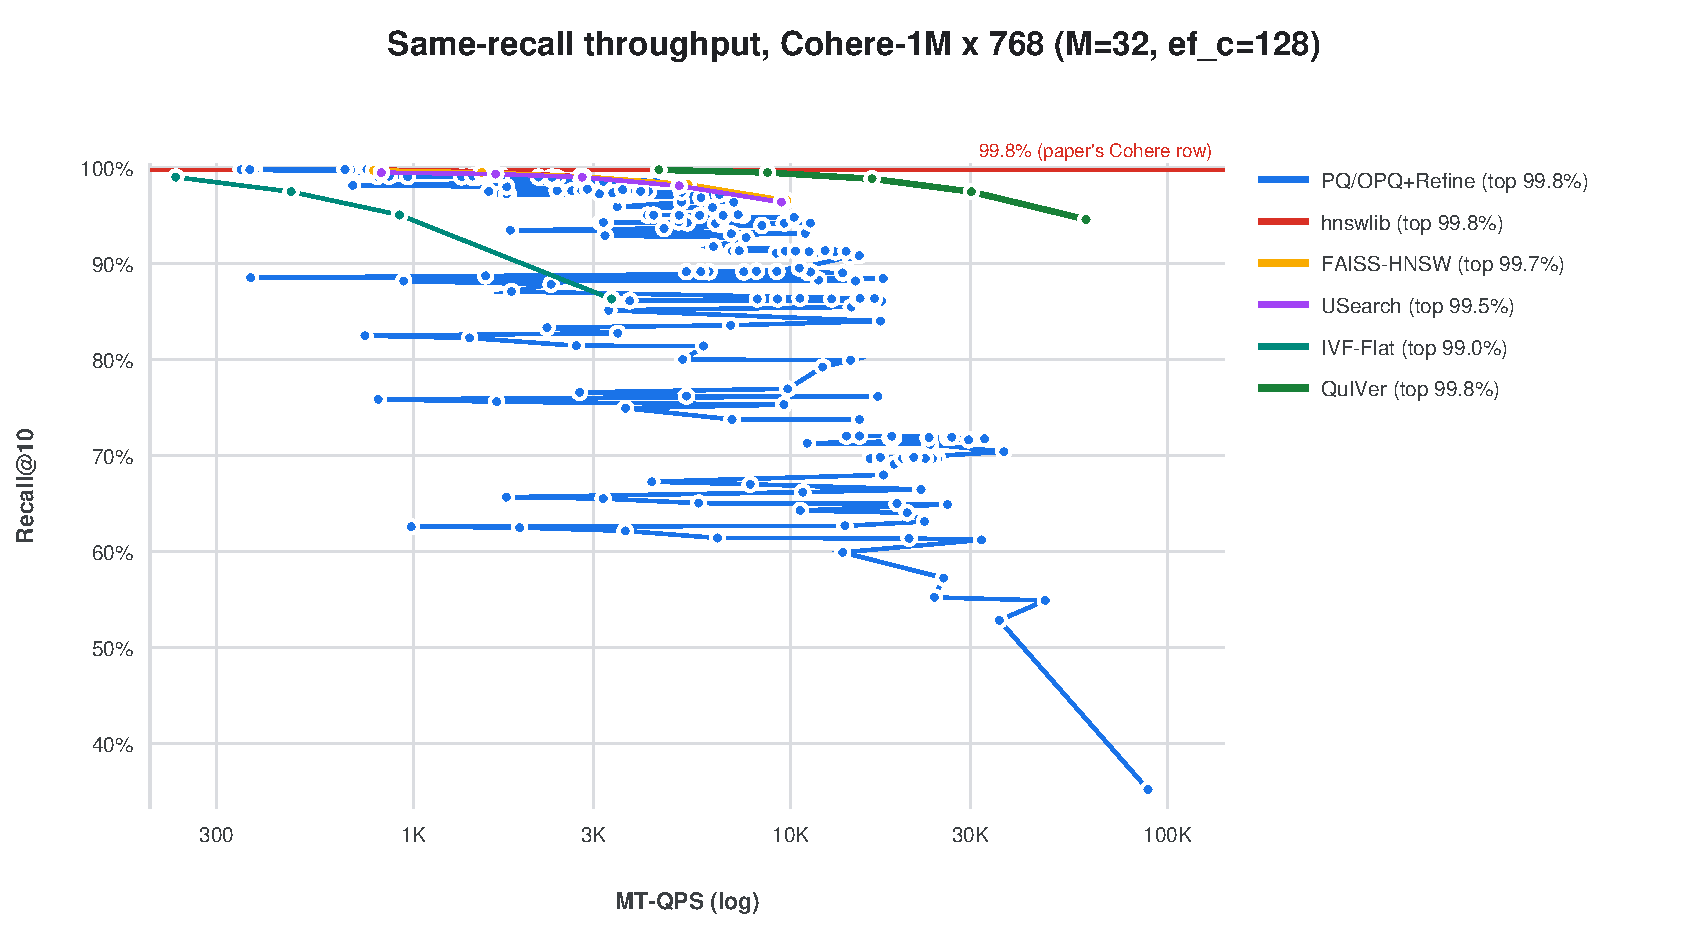
\includegraphics[keepaspectratio,alt={Figure 5.
Same-recall throughput on Cohere-1M $\times$ 768: QuIVer against the HNSW
family and OPQ+IVF-PQ+Refine. At $\geq$ 99 \% recall QuIVer is 3.7$\times$ faster
than the refined PQ pipeline, which is the only competitor class that
reaches the same ceiling.}]{figures/fig5-matched-recall.pdf}}
\caption{\textbf{Figure 5.} Same-recall throughput on Cohere-1M $\times$ 768:
QuIVer against the HNSW family and OPQ+IVF-PQ+Refine. At $\geq$ 99 \% recall
QuIVer is 3.7$\times$ faster than the refined PQ pipeline, which is the only
competitor class that reaches the same ceiling.}
\end{figure}

\textbf{(b) The same-family arm, and the protocol trap that faked its
verdict.} The paper's list also names its own family --- ``FAISS
IVF+RaBitQ+Refine'' --- so we ran \texttt{IndexIVFRaBitQ} +
\texttt{IndexRefineFlat} (f32 re-ranking) on Cohere-1M alongside an
exact IVF-Flat arm on the same nprobe grid. The first run produced a
result that is \emph{impossible} if both arms are measured correctly:
under the same ground truth, the exact-coarse arm saturated at
\textbf{34.9 \%} while the candidate-pool arm reached \textbf{59.8--60.2
\%} --- although every refine result re-ranks a subset of what IVF-Flat
compares exactly, so IVF-Flat must be the upper bound. We did not
publish either number, and diagnosed before writing. Three checks
resolved it (all artifacts ship with the draft):

\begin{enumerate}
\def\labelenumi{\arabic{enumi}.}
\tightlist
\item
  \textbf{The parameters were reaching the index.}
  \texttt{ParameterSpace().set\_index\_parameter(wrapper,\ "nprobe",\ x)}
  is verified to land on the wrapped base (\texttt{base.nprobe\ =\ 256}
  after the call). The one real parameter bug was \texttt{k\_factor}: it
  is \emph{not} settable through \texttt{ParameterSpace} in faiss 1.15,
  and the pre-fix script's \texttt{except:\ pass} silently kept the
  default (\texttt{k\_factor\ =\ 1}) --- the tell was that the earlier
  sweep printed \emph{identical} recalls for every \texttt{k\_factor}
  value, with only the small nprobe slope. The fixed script assigns
  directly and records the \textbf{effective} values
  (\texttt{eff\_nprobe}, \texttt{eff\_k\_factor}) in every artifact row.
\item
  \textbf{FAISS behaves as theory demands on a controlled task.} On
  synthetic data with a self-consistent GT, larger \texttt{k\_factor}
  monotonically improves the refine arm (19.3 $\rightarrow$ 44.5 $\rightarrow$ 46.1 \%), and at
  \texttt{k\_factor\ =\ 200} it \emph{equals} the exact IVF-Flat control
  at the same nprobe (46.05 \% = 46.05 \%). The inversion is not a
  library defect.
\item
  \textbf{The ground truth does not match the on-disk vectors.} The
  shipped Cohere GT is reproduced exactly by inner product on
  \textbf{normalised} vectors (10.0/10 overlap on six queries) and
  cannot be reproduced by raw-vector search (raw-IP 4.2/10; the f32
  files carry $\|$x$\|$ $\approx$ 13.8 --- Cohere is the one dataset our preparation
  pipeline left un-normalised, while its GT is cosine). Every raw-vector
  arm is scored against the wrong objective --- and the two sub-arms
  fail \emph{differently} against it: a small candidate pool follows the
  RaBitQ code's direction-based estimate (which happens to track cosine
  better, hence ``60 \%''), while a larger pool lets the f32 re-ranking
  drag the result toward the raw-IP answer (hence 35 \%, converging to
  the exact arm's 34.8 \%).
\end{enumerate}

\textbf{Corrected measurement (normalised vectors, same GT, 32 threads,
idle machine):}

{\def\LTcaptype{none} % do not increment counter
\begin{longtable}[]{@{}
  >{\raggedright\arraybackslash}p{(\linewidth - 8\tabcolsep) * \real{0.2000}}
  >{\raggedright\arraybackslash}p{(\linewidth - 8\tabcolsep) * \real{0.2000}}
  >{\raggedright\arraybackslash}p{(\linewidth - 8\tabcolsep) * \real{0.2000}}
  >{\raggedright\arraybackslash}p{(\linewidth - 8\tabcolsep) * \real{0.2000}}
  >{\raggedright\arraybackslash}p{(\linewidth - 8\tabcolsep) * \real{0.2000}}@{}}
\toprule\noalign{}
\begin{minipage}[b]{\linewidth}\raggedright
Arm
\end{minipage} & \begin{minipage}[b]{\linewidth}\raggedright
nprobe = 64
\end{minipage} & \begin{minipage}[b]{\linewidth}\raggedright
256
\end{minipage} & \begin{minipage}[b]{\linewidth}\raggedright
512
\end{minipage} & \begin{minipage}[b]{\linewidth}\raggedright
1024 (full scan)
\end{minipage} \\
\midrule\noalign{}
\endhead
\bottomrule\noalign{}
\endlastfoot
IVF-Flat, exact coarse (upper bound) & 97.38 \% @ 279 & 99.82 \% @ 72 &
99.98 \% @ 37 & \textbf{100.00 \%} @ 21 \\
RaBitQ+Refine, \texttt{k\_factor\ =\ 1} (default) & 78.03 \% @ 4,656 &
78.88 \% @ 1,272 & 78.90 \% @ 673 & 78.91 \% @ 369 \\
RaBitQ+Refine, \texttt{k\_factor\ =\ 20} & 97.37 \% @ 4,364 & 99.79 \% @
1,268 & 99.95 \% @ 673 & 99.97 \% @ 380 \\
RaBitQ+Refine, \texttt{k\_factor\ =\ 200} & 97.38 \% @ 2,885 & 99.82 \%
@ 1,087 & 99.98 \% @ 611 & \textbf{100.00 \%} @ 360 \\
\end{longtable}
}

Three readings. (i) \textbf{The inversion is gone}: at every nprobe the
candidate-pool arm is $\leq$ the exact arm and ties it once the pool covers
the probed lists --- the family ranks exactly as theory requires. (ii) A
``same-family'' arm must \textbf{document its effective parameters}: the
default \texttt{k\_factor\ =\ 1} sits \textasciitilde19 pp below the
tuned point at the same nprobe, and pre-fix artifacts that hide it are
not baselines. (iii) As a deployment datum the family is real: at $\approx$ 97.4
\% recall the refine arm recovers the exact arm's recall at \textbf{$\approx$
15$\times$} its QPS (4,364 vs 279), and at $\approx$ 99.8 \% it is still $\approx$ 15$\times$ (1,087
vs 72). The retracted raw-vector pair is kept in the artifact store,
flagged, as the record of the trap; a normalised FastScan+SQ8 spot check
from the same family reaches 98.99 \% at nprobe = 256 /
\texttt{k\_factor} = 20 (recall-only log).

\textbf{(c) The third axis: bit capacity, not data difficulty.} Holding
the code family fixed and varying only bits per dimension (§6.5) moves
every one of the four ``collapse'' datasets from $\leq$ 3.6 \% (1--2 bit) to
\textbf{$\geq$ 94.6 \% (4 bit)} on the same task. So ``collapse'' is mostly
\emph{this} 2-bit allocation, not the distribution: the axis the paper
varies is the dataset, while the axis that moves the outcome is the
code's bit budget.

\section{6. Diagnosis: Why the Code Fails, and Three Different
Failures}\label{diagnosis-why-the-code-fails-and-three-different-failures}

\begin{quote}
Notation as in §4. \emph{Sign plane} = the
\texttt{pos\ =\ (v\ \textgreater{}\ 0)} plane; \emph{magnitude plane} =
the
\texttt{strong\ =\ (\textbar{}v\textbar{}\ \textgreater{}\ mean\textbar{}v\textbar{})}
plane.
\end{quote}

\subsection{6.1 The mechanism, in one
identity}\label{the-mechanism-in-one-identity}

QuIVer's weighted distance is a monotone transform of

\begin{verbatim}
S(a,b) = <w_a, w_b>,   where   w = (2p - 1) * (1 + s) in {-2, -1, +1, +2}
\end{verbatim}

We verified this against the implementation bit-for-bit
(\texttt{bq2\_code\_ceiling.py::verify\_identities}, max
\textbar analytic $-$ bitwise\textbar{} = 0). Two consequences follow
immediately.

\textbf{If the sign plane is constant}, \texttt{p\ $\equiv$\ 0} for every
dimension, so \texttt{w\ =\ $-$(1\ +\ s)} and

\begin{verbatim}
S(a,b) = <1 + s_a, 1 + s_b>  =  D + <s_a, s_b>  + sum(s_a + s_b)
\end{verbatim}

i.e.~the ordering is dominated by the \textbf{magnitude statistics} of
the two codes, not by their direction. On GIST-960 we measure the
resulting bias at \textbf{+3.34 $\sigma$} of the true (cosine) score spread,
and the \texttt{pos}-plane Hamming rate at \textbf{0.0000} --- the sign
plane carries \textbf{zero} bits of information.

\textbf{If the sign plane is alive}, the weighted score is a genuine
two-plane match and the ordering tracks cosine. This is why the repair
in §8 works at all, and why it is \emph{data-dependent} rather than
universal.

\subsection{\texorpdfstring{6.2 Quantifying ``alive'':
\texttt{sign\_info}}{6.2 Quantifying ``alive'': sign\_info}}\label{quantifying-alive-sign_info}

We summarise the sign plane by the mean per-coordinate sign entropy

\begin{verbatim}
sign_info = mean_j H(p_j),   p_j = P(v_j < 0),   H(p) = -p log_2 p - (1-p) log_2(1-p)   [bits]
\end{verbatim}

On \textbf{22 arms} (12 paper datasets + centred variants + planted
controls) the distribution is \emph{bimodal with a wide gap}:
\texttt{sign\_info\ =\ 0.000} exactly for \texttt{gist960} (at
128/256/512/768/960 dims) and \texttt{sift128}, and \textbf{0.597 --
1.000} for every other arm. This is the quantity that distinguishes
``the code is being asked to do something it cannot do'' from ``the task
itself is hard'' --- see §6.4.

\emph{Negative result we report:} the per-coordinate \textbf{minimum}
\texttt{min\_j\ H(p\_j)} is \textbf{not} usable --- it fires on healthy
data (Cohere, R@10 97.51 \%, has \texttt{min\_j\ H(p\_j)\ =\ 0.000}
because a few coordinates are pinned by a strong mean direction). Only
the \emph{mean} separates.

\subsection{6.3 The graph is faithful to the wrong
metric}\label{the-graph-is-faithful-to-the-wrong-metric}

For each dataset we exported the L0 adjacency (CSR,
\texttt{bench\_t2\_build\_recon}) and measured its overlap with the true
top-64 under three metrics (256 sampled nodes, self-loops excluded):

{\def\LTcaptype{none} % do not increment counter
\begin{longtable}[]{@{}
  >{\raggedright\arraybackslash}p{(\linewidth - 10\tabcolsep) * \real{0.1667}}
  >{\raggedright\arraybackslash}p{(\linewidth - 10\tabcolsep) * \real{0.1667}}
  >{\raggedright\arraybackslash}p{(\linewidth - 10\tabcolsep) * \real{0.1667}}
  >{\raggedright\arraybackslash}p{(\linewidth - 10\tabcolsep) * \real{0.1667}}
  >{\raggedright\arraybackslash}p{(\linewidth - 10\tabcolsep) * \real{0.1667}}
  >{\raggedright\arraybackslash}p{(\linewidth - 10\tabcolsep) * \real{0.1667}}@{}}
\toprule\noalign{}
\begin{minipage}[b]{\linewidth}\raggedright
Dataset
\end{minipage} & \begin{minipage}[b]{\linewidth}\raggedright
Tier
\end{minipage} & \begin{minipage}[b]{\linewidth}\raggedright
\textbf{L0 $\cap$ cos\_top64}
\end{minipage} & \begin{minipage}[b]{\linewidth}\raggedright
L0 $\cap$ w\_top64 (\textbf{build} metric)
\end{minipage} & \begin{minipage}[b]{\linewidth}\raggedright
L0 $\cap$ cheap\_top64 (\textbf{query} metric)
\end{minipage} & \begin{minipage}[b]{\linewidth}\raggedright
measured R@10 @128
\end{minipage} \\
\midrule\noalign{}
\endhead
\bottomrule\noalign{}
\endlastfoot
Cohere-768 & competitive & \textbf{56.84 \%} & 77.84 \% & 62.82 \% &
97.51 \% \\
MiniLM-384 & competitive & \textbf{65.80 \%} & 82.10 \% & 58.11 \% &
94.28 \% \\
Wolt-CLIP-512 & moderate & \textbf{53.19 \%} & 72.40 \% & 58.50 \% &
77.73 \% \\
GloVe-100 & usable & \textbf{31.82 \%} & 64.24 \% & 20.78 \% & 45.60
\% \\
GIST-960 (centred) & repaired & \textbf{27.98 \%} & 53.60 \% & 30.07 \%
& 51.96 \% \\
SIFT-128 & collapse & \textbf{4.34 \%} & 60.99 \% & 17.00 \% & 21.88
\% \\
GIST-960 & collapse & \textbf{1.01 \%} & 65.62 \% & 0.79 \% & 2.81 \% \\
Gaussian-960 (control) & index-agnostic & 4.67 \% & 7.13 \% & 1.80 \% &
0.83 \% \\
Gaussian-960 + planted NN & positive control & 4.47 \% & 7.24 \% & 1.84
\% & \textbf{100.00 \%} \\
\end{longtable}
}

Three readings:

\begin{enumerate}
\def\labelenumi{\arabic{enumi}.}
\tightlist
\item
  \textbf{The index executes its instructions.} \texttt{L0\ $\cap$\ w\_top64}
  is 53--82 \% everywhere, while \texttt{L0\ $\cap$\ cos\_top64} spans
  \textbf{1.01 \% $\rightarrow$ 65.80 \%}. Collapse rows have graphs that are
  \emph{cosine-random} (GIST 1.01 \%), not badly built graphs.
\item
  \textbf{Fidelity tracks recall across 9 datasets} (1.01$\rightarrow$2.81,
  4.34$\rightarrow$21.88, 27.98$\rightarrow$51.96, 31.82$\rightarrow$45.60, 53.19$\rightarrow$77.73, 56.84$\rightarrow$97.51,
  65.80$\rightarrow$94.28) --- it is closer to the real bottleneck than any
  code-side probe.
\item
  \textbf{But it is not sufficient}: the planted-NN control reaches
  \textbf{100 \%} recall with 4.47 \% fidelity (the planted neighbours
  are so close that even a bad graph finds them). Consistent with our
  two failed single-scalar predictors (§7.4): there is no one quantity
  that predicts everything.
\end{enumerate}

\subsection{6.4 Three different failures inside the paper's
``\textless{} 15 \%''
tier}\label{three-different-failures-inside-the-papers-15-tier}

The competitor curves we ran on the \emph{same} tasks (§8.4) plus the
VIBE row \texttt{coco\_nomic} (§9.5) reveal that the paper's bottom tier
mixes three phenomena with three different deployment answers:

{\def\LTcaptype{none} % do not increment counter
\begin{longtable}[]{@{}
  >{\raggedright\arraybackslash}p{(\linewidth - 6\tabcolsep) * \real{0.2500}}
  >{\raggedright\arraybackslash}p{(\linewidth - 6\tabcolsep) * \real{0.2500}}
  >{\raggedright\arraybackslash}p{(\linewidth - 6\tabcolsep) * \real{0.2500}}
  >{\raggedright\arraybackslash}p{(\linewidth - 6\tabcolsep) * \real{0.2500}}@{}}
\toprule\noalign{}
\begin{minipage}[b]{\linewidth}\raggedright
\end{minipage} & \begin{minipage}[b]{\linewidth}\raggedright
\textbf{(i) Code-specific collapse}
\end{minipage} & \begin{minipage}[b]{\linewidth}\raggedright
\textbf{(ii) Index-agnostic collapse}
\end{minipage} & \begin{minipage}[b]{\linewidth}\raggedright
\textbf{(iii) Capacity collapse}
\end{minipage} \\
\midrule\noalign{}
\endhead
\bottomrule\noalign{}
\endlastfoot
Representatives & GIST-960, SIFT-128 & Random-Sphere-1M, Gaussian-960 &
\texttt{coco\_nomic} (VIBE, 768-d) \\
\texttt{sign\_info} & \textbf{0.000} & \textbf{1.000} &
\textbf{0.382} \\
HNSW \texttt{ef=64}, same task & \textbf{normal}: 84.11 \% / 97.06 \% &
\textbf{also collapses: 1.40 \% (Random-Sphere) / 1.10--1.39 \%
(Gaussian-960, three implementations)} & \textbf{normal: 86.23 \%} @
17,053 \\
Centring & \textbf{+37.6 / +14.9 pp} (2.10$\rightarrow$39.74, 15.77$\rightarrow$30.64 @ef\_s=64)
& \textbf{+0.03 pp} (0.48$\rightarrow$0.51) & helps little (still 2-bit) \\
Seeded rotation (task-preserving) & \textbf{+58.1 / +44.5 pp}
(2.10$\rightarrow$60.22 @ef=64) & no gain (report: +0.03 pp) & \textbf{useless: 0.21
$\rightarrow$ 0.70 \%} \\
PQ/OPQ+Refine, same task & --- (not measured) & --- (not measured) &
\textbf{98.42 \%} @ 7,771 \\
4-bit uniform code + re-rank & 99.05 \% & \textbf{99.30 \%} & 94.60
\% \\
\texttt{L0\ $\cap$\ cos\_top64} & 1.01 \% / 4.34 \% (27.98 \% centred) & 4.67
\% & --- \\
What a deployer should do & centre \textbf{or} rotate --- and still
prefer HNSW unless a 2--5 pp gap is acceptable & \textbf{do not build a
graph index on this task} & \textbf{change the code} (PQ pays 4.7$\times$
memory) or accept the loss \\
\end{longtable}
}

\textbf{A second witness for (ii).} On Gaussian-960 we ran the full
competitor set on the same task: hnswlib \textbf{1.10 \%}, FAISS-HNSW
\textbf{1.30 \%}, USearch \textbf{1.39 \%}, and IVF-Flat \textbf{2.41
\%} at \texttt{ef=64} --- with every curve still $\leq$ 19 \% at
\texttt{ef=1024}. Four independent indexes agree that this task has no
usable neighbourhood structure, so the index-agnostic reading is not an
artefact of one HNSW implementation.

The paper answers all three with one sentence (``use float32''), which
is correct as far as it goes but hides that (i) is an \emph{encoding}
problem that can be repaired, (ii) is a \emph{task} problem that cannot,
and (iii) is a \emph{capacity} problem where the fix is a different code
--- the one remedy that gives up the 675 MiB advantage this index exists
for. \texttt{sign\_info} separates (i) from (ii) for free, before any
index is built; (iii) is the case where both planes are partially alive
and no pre-index statistic we tested separates it (§7.4).

\subsection{6.5 The axis that actually moves the outcome: bits per
dimension}\label{the-axis-that-actually-moves-the-outcome-bits-per-dimension}

To test whether ``collapse'' is a property of the data or of the code,
hold the code family fixed and vary only the budget. Instrument:
per-dimension uniform quantization at \emph{b} bits (min/max scaled),
re-ranked exactly in float32 over the code's top-128 (\texttt{ef=128},
200 K sampled base vectors, 200 queries) --- the same instrument as the
paper's own probe (§7.1), with the resolution turned into a variable
(Figure 6).

{\def\LTcaptype{none} % do not increment counter
\begin{longtable}[]{@{}
  >{\raggedright\arraybackslash}p{(\linewidth - 12\tabcolsep) * \real{0.1429}}
  >{\raggedright\arraybackslash}p{(\linewidth - 12\tabcolsep) * \real{0.1429}}
  >{\raggedright\arraybackslash}p{(\linewidth - 12\tabcolsep) * \real{0.1429}}
  >{\raggedright\arraybackslash}p{(\linewidth - 12\tabcolsep) * \real{0.1429}}
  >{\raggedright\arraybackslash}p{(\linewidth - 12\tabcolsep) * \real{0.1429}}
  >{\raggedright\arraybackslash}p{(\linewidth - 12\tabcolsep) * \real{0.1429}}
  >{\raggedright\arraybackslash}p{(\linewidth - 12\tabcolsep) * \real{0.1429}}@{}}
\toprule\noalign{}
\begin{minipage}[b]{\linewidth}\raggedright
Dataset (tier the paper assigns)
\end{minipage} & \begin{minipage}[b]{\linewidth}\raggedright
1 bit
\end{minipage} & \begin{minipage}[b]{\linewidth}\raggedright
\textbf{2 bit}
\end{minipage} & \begin{minipage}[b]{\linewidth}\raggedright
3 bit
\end{minipage} & \begin{minipage}[b]{\linewidth}\raggedright
\textbf{4 bit}
\end{minipage} & \begin{minipage}[b]{\linewidth}\raggedright
6 bit
\end{minipage} & \begin{minipage}[b]{\linewidth}\raggedright
16 bit
\end{minipage} \\
\midrule\noalign{}
\endhead
\bottomrule\noalign{}
\endlastfoot
GIST-960 (collapse) & 3.55 \% & \textbf{55.25 \%} & 60.25 \% &
\textbf{99.05 \%} & 99.95 \% & 100 \% \\
Gaussian-960 (index-agnostic collapse) & 21.85 \% & \textbf{23.05 \%} &
76.10 \% & \textbf{99.50 \%} & 100 \% & 100 \% \\
Random-Sphere (collapse) & 20.85 \% & \textbf{23.25 \%} & 76.75 \% &
\textbf{99.30 \%} & 100 \% & 100 \% \\
\texttt{coco\_nomic} (capacity collapse) & 9.75 \% & \textbf{31.60 \%} &
76.10 \% & \textbf{94.60 \%} & 99.00 \% & 100 \% \\
\end{longtable}
}

Three consequences, in order of how much they change the paper's
wording:

\begin{enumerate}
\def\labelenumi{\arabic{enumi}.}
\tightlist
\item
  \textbf{All four ``collapse'' datasets are $\geq$ 94.6 \% at 4 bits.} The
  bottom tier is largely ``2 bits per dimension cannot hold this
  distribution'', not ``this dataset cannot be quantized''.
\item
  \textbf{The 2-bit sign--magnitude scheme is worse than naïve 2-bit
  uniform quantization} on the datasets where both exist:
  \texttt{coco\_nomic} 3.59 \% measured vs \textbf{31.60 \%} in this
  table; Gaussian-960 0.83 \% vs \textbf{23.05 \%}. Spending one of the
  two bits on an almost-constant sign plane has a measurable price, and
  it is the quantity our repairs (centre / rotate) recover
  \emph{without} adding bits.
\item
  \textbf{Random-Sphere's failure is not (only) in the code.} A 4-bit
  code with exact re-ranking reaches 99.30 \% on that task, yet HNSW
  collapses (1.40 \%) --- so its problem is in the \emph{graph},
  consistent with §6.3's fidelity instrument. Only the code-side
  statistic and the graph-side statistic \emph{together} separate the
  three failure types, which is why §7's chain uses both.
\end{enumerate}

\textbf{Scope.} The 1-bit row of this table is \textbf{naïve 1-bit
uniform}, and is \emph{not} QuIVer's 1-bit ablation; it is reported to
bracket the axis, not as a competing implementation. The 16-bit row is
the float32-equivalent upper bound (100 \% by construction, up to tie
degeneracy).

\begin{figure}
\centering
\pandocbounded{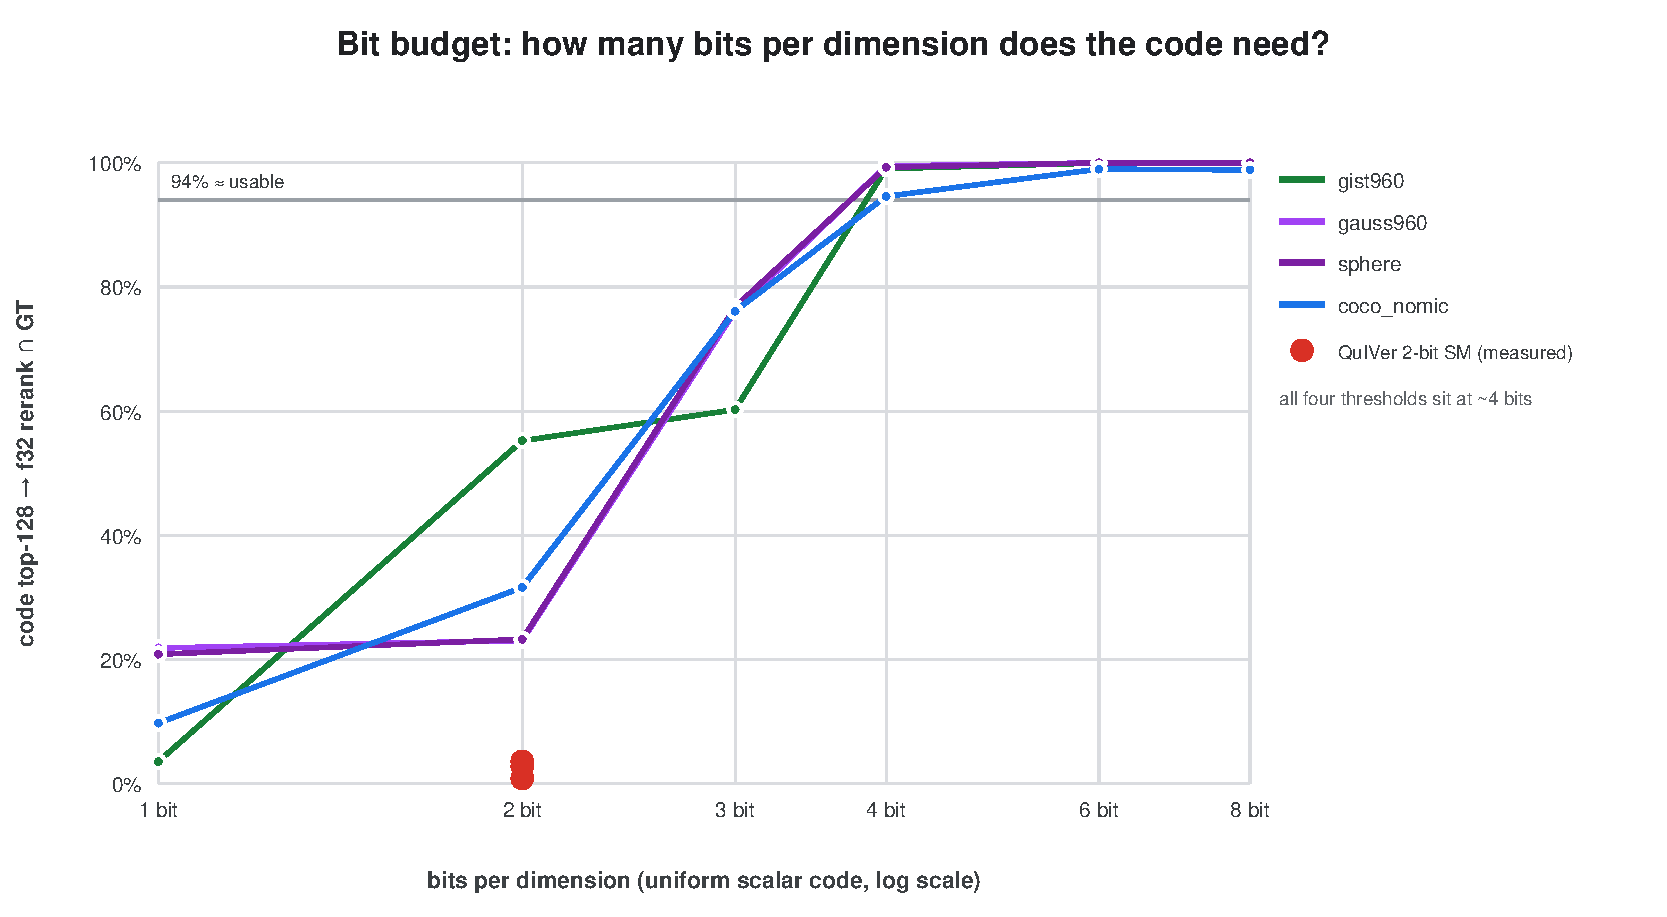
\includegraphics[keepaspectratio,alt={Figure 6. Bits per
dimension vs achievable recall for a uniform scalar code with exact f32
re-ranking over the code's top-128 (200 K base / 200 queries, four
collapse datasets). All four cross $\approx$ 94 \% at 4 bits; the red markers
are the shipped 2-bit sign--magnitude code measured on the same
tasks.}]{figures/fig6-bit-budget.pdf}}
\caption{\textbf{Figure 6.} Bits per dimension vs achievable recall for
a uniform scalar code with exact f32 re-ranking over the code's top-128
(200 K base / 200 queries, four collapse datasets). All four cross $\approx$ 94
\% at 4 bits; the red markers are the shipped 2-bit sign--magnitude code
measured on the same tasks.}
\end{figure}

\section{7. The Judge: Three Specification Gaps, and a Repaired
Chain}\label{the-judge-three-specification-gaps-and-a-repaired-chain}

\begin{quote}
We do \textbf{not} claim the paper's probe is wrong. We claim it is
\textbf{under-specified}, and we measure what the specification gaps
cost.
\end{quote}

\subsection{7.1 What is specified, and what is
not}\label{what-is-specified-and-what-is-not}

§6 of the paper (``Practical compatibility test'') states: take $\approx$10 K
sample vectors, rank them by the BQ code, compare with the float32
ranking by top-K overlap, and read \textbf{\textgreater{}
\textasciitilde50 \% $\Rightarrow$ compatible, \textless{} 50 \% $\Rightarrow$ use a float32
index}. It needs no index. Three things are left open:

{\def\LTcaptype{none} % do not increment counter
\begin{longtable}[]{@{}
  >{\raggedright\arraybackslash}p{(\linewidth - 2\tabcolsep) * \real{0.5000}}
  >{\raggedright\arraybackslash}p{(\linewidth - 2\tabcolsep) * \real{0.5000}}@{}}
\toprule\noalign{}
\begin{minipage}[b]{\linewidth}\raggedright
gap
\end{minipage} & \begin{minipage}[b]{\linewidth}\raggedright
why it matters
\end{minipage} \\
\midrule\noalign{}
\endhead
\bottomrule\noalign{}
\endlastfoot
\textbf{which} BQ distance & the engine has two: \texttt{weighted}
(6-class, used for build/prune/upper layers) and \texttt{cheap} (plain
Hamming, used for L0 query navigation) \\
sample \textbf{source and size} & base only, or base+queries? how
many? \\
the \textbf{instrument} & ``BQ-ranked Top-10'' (literal) vs ``code
top-\emph{ef} $\rightarrow$ f32 re-rank'' (what a graph search actually does) \\
\end{longtable}
}

\subsection{7.2 What the gaps cost
(measured)}\label{what-the-gaps-cost-measured}

\textbf{(a) The metric flips the verdict, and can produce a false
positive.} Implemented exactly as written with the paper's own default
metric (\texttt{weighted}), the probe returns

{\def\LTcaptype{none} % do not increment counter
\begin{longtable}[]{@{}
  >{\raggedright\arraybackslash}p{(\linewidth - 6\tabcolsep) * \real{0.2500}}
  >{\raggedright\arraybackslash}p{(\linewidth - 6\tabcolsep) * \real{0.2500}}
  >{\raggedright\arraybackslash}p{(\linewidth - 6\tabcolsep) * \real{0.2500}}
  >{\raggedright\arraybackslash}p{(\linewidth - 6\tabcolsep) * \real{0.2500}}@{}}
\toprule\noalign{}
\begin{minipage}[b]{\linewidth}\raggedright
dataset
\end{minipage} & \begin{minipage}[b]{\linewidth}\raggedright
probe (\texttt{weighted}, top-ef)
\end{minipage} & \begin{minipage}[b]{\linewidth}\raggedright
probe (\texttt{min(w,\ cheap)}, top-ef)
\end{minipage} & \begin{minipage}[b]{\linewidth}\raggedright
measured R@10 @ef=64
\end{minipage} \\
\midrule\noalign{}
\endhead
\bottomrule\noalign{}
\endlastfoot
\textbf{Random-Sphere-1M} & \textbf{53.9 \% $\Rightarrow$ ``compatible''} &
\textbf{4.9 \% $\Rightarrow$ ``use float32''} & \textbf{0.91 \%} (paper: 0.40 \%) \\
\textbf{Gaussian-960} (our control) & \textbf{55.0 \% $\Rightarrow$ ``compatible''}
& \textbf{4.7 \% $\Rightarrow$ ``use float32''} & \textbf{0.83 \%} \\
\end{longtable}
}

So the verdict is \emph{go} or \emph{no-go} depending on an unstated
choice --- and the \texttt{weighted} reading is a false positive on
\textbf{two} datasets whose actual recall is under 1 \%. Taking the
weaker of the two metrics repairs both without changing any other arm's
verdict (a third instance of the same ambiguity, measured with the
literal top-10 instrument, is Synthetic-LR: \texttt{weighted} 66.95 \%
vs \texttt{cheap} 45.25 \% --- opposite verdicts on the same data).

\textbf{(b) The probe is strongly sample-size dependent.} Sweeping the
candidate sample size changes the probe value by up to \textbf{6.8$\times$},
and the direction is systematic: \emph{fewer samples $\Rightarrow$ more optimistic}.
Independently, different query subsets give a \textbf{4--7 pp} spread,
so a single-run number is not quotable.

\begin{figure}
\centering
\pandocbounded{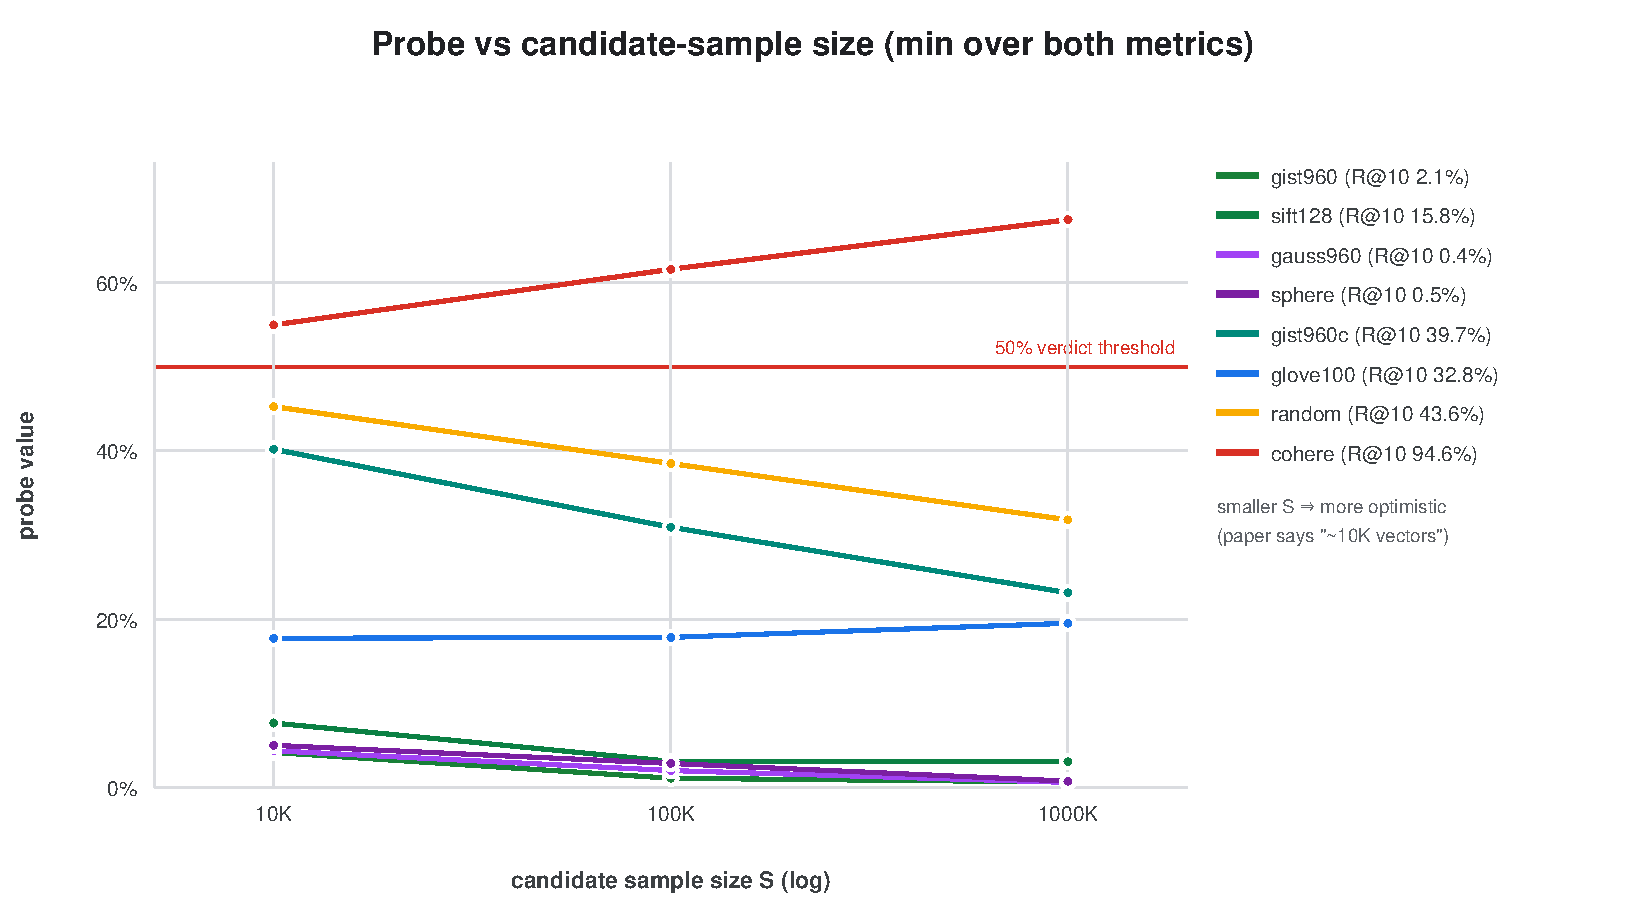
\includegraphics[keepaspectratio,alt={Figure 4. The
published probe (min over the two BQ metrics) as a function of candidate
sample size S for eight arms (legend: measured R@10 at ef=64). Smaller S
is systematically more optimistic; the paper's ``$\approx$ 10K vectors''
prescription sits at the top of a curve whose total swing is 6.8$\times$ (see
also (c)).}]{figures/fig4-probe-sample-size.pdf}}
\caption{\textbf{Figure 4.} The published probe (min over the two BQ
metrics) as a function of candidate sample size \protect\texttt{S} for
eight arms (legend: measured R@10 at \protect\texttt{ef=64}). Smaller
\protect\texttt{S} is systematically more optimistic; the paper's ``$\approx$
10K vectors'' prescription sits at the top of a curve whose total swing
is 6.8$\times$ (see also (c)).}
\end{figure}

\textbf{(c) The literal instrument is pessimistic.} ``Code top-10 $\cap$ f32
GT'' understates what a graph search achieves, because search uses the
code to \emph{navigate} and then re-ranks \texttt{ef} candidates in
float32. GIST-960 (centred) is the clearest case: top-10 gives
\textbf{25.4--29.8 \%} while the \texttt{top-ef} instrument gives
\textbf{70.5 \%}, against a measured recall of \textbf{51.96 \%}. On
GloVe-100 the \texttt{top-ef} instrument returns \textbf{44.8 \%}
against a measured \textbf{45.60 \%}, and on Cohere \textbf{98.7 \%}
against \textbf{97.51 \%}. In the P2 analysis the \texttt{code\_oracle}
variant of this instrument tracked recall at $\rho$ = +0.95; we therefore
report the \texttt{top-ef} instrument and never a single-run
\texttt{top-10} value as a usability verdict.

\subsection{7.3 The repaired chain}\label{the-repaired-chain}

Four quantities, all computable in seconds and \textbf{before building
any index}:

\begin{verbatim}
(1) sign_info  < 0.2                     => rotate (Sec. 8.6; task-preserving) or centre — the sign plane is globally degenerate
(2) ||mu|| >= 0.3 and headroom > 5 pp        => centre as well (the shift is large and there is room to gain)
(3) probe_ef (min over both metrics,
   code top-128 -> f32 re-rank) < 50 %  => use a float32 index
(4) otherwise                            => BQ-native is usable (competitiveness is *not* predicted here)
\end{verbatim}

Validated on \textbf{22 arms: 21 defensible verdicts} (the table in
\texttt{results/t2/deployability\_gate.json}; the bimodal gap that makes
rule (1) work is \texttt{sign\_info\ =\ 0.000} for the six GIST/SIFT arms
vs \textbf{$\geq$ 0.597} for all other 18). The single boundary case is
centred GloVe-100 (\texttt{probe\_ef} = 44.9 \% against a 50 \%
threshold), where ``use float32'' happens to be right for a
\emph{different} reason (it is dominated by HNSW anyway, §8.4).

\textbf{Sampling stability.} Instrument values are means over \textbf{K
= 5 disjoint query subsets} (the artifact table carries
\texttt{probe\_k\ =\ 5}). Re-run against the K = 3 version of the same
table, \textbf{no verdict changes} and no arm drifts by more than
\textbf{1.7 pp} (\texttt{sift128r}; 0 of 38 arms exceed a 3 pp
threshold) --- the chain is not an artifact of an unlucky sample, which
was the main way a 200-query probe could have failed.

\textbf{Prospective validation (the part that is not circular).} The
rule ``open weighted navigation iff
\texttt{probe\_ef(weighted)\ \textgreater{}\ probe\_ef(Hamming)}'' was
frozen \emph{before} the six arms below were measured; none took part in
fitting it, and all six follow the prediction --- including both large
forks:

{\def\LTcaptype{none} % do not increment counter
\begin{longtable}[]{@{}
  >{\raggedright\arraybackslash}p{(\linewidth - 8\tabcolsep) * \real{0.2000}}
  >{\raggedright\arraybackslash}p{(\linewidth - 8\tabcolsep) * \real{0.2000}}
  >{\raggedright\arraybackslash}p{(\linewidth - 8\tabcolsep) * \real{0.2000}}
  >{\raggedright\arraybackslash}p{(\linewidth - 8\tabcolsep) * \real{0.2000}}
  >{\raggedright\arraybackslash}p{(\linewidth - 8\tabcolsep) * \real{0.2000}}@{}}
\toprule\noalign{}
\begin{minipage}[b]{\linewidth}\raggedright
arm (held out)
\end{minipage} & \begin{minipage}[b]{\linewidth}\raggedright
probe weighted / Hamming
\end{minipage} & \begin{minipage}[b]{\linewidth}\raggedright
rule says
\end{minipage} & \begin{minipage}[b]{\linewidth}\raggedright
measured w0 $\rightarrow$ w1 @ef=64
\end{minipage} & \begin{minipage}[b]{\linewidth}\raggedright
$\Delta$
\end{minipage} \\
\midrule\noalign{}
\endhead
\bottomrule\noalign{}
\endlastfoot
\texttt{arxiv\_nomic} & 99.5 \% / 99.5 \% & plain & 96.78 \% $\rightarrow$ 96.04 \%
& $-$0.74 \\
\texttt{codesearch\_jina} & 99.9 \% / 99.9 \% & weighted & 94.62 \% $\rightarrow$
\textbf{96.37 \%} & +1.75 \\
\texttt{gooaq\_roberta} & 100.0 \% / 99.7 \% & weighted & 96.60 \% $\rightarrow$
\textbf{98.32 \%} & +1.72 \\
\texttt{landmark\_nomic} & 93.7 \% / \textbf{99.6 \%} & plain & 93.05 \%
$\rightarrow$ \textbf{81.39 \%} & \textbf{$-$11.66} \\
\texttt{landmark\_dino} & \textbf{99.2 \%} / 96.2 \% & weighted & 82.90
\% $\rightarrow$ \textbf{91.58 \%} & \textbf{+8.68} \\
\texttt{gist960rc} & 99.6 \% / 95.6 \% & weighted & 76.05 \% $\rightarrow$
\textbf{80.17 \%} & +4.12 \\
\end{longtable}
}

\textbf{6/6 prospective} (5/6 in the fitting set; the miss is Wolt-CLIP
at $-$0.5 pp / +0.9 pp, inside the §3.5 noise floor) $\Rightarrow$ \textbf{11/12
overall}, with both large forks called in advance. Note the rule
predicts the \emph{sign} of the navigation-metric choice, not its
magnitude: \texttt{landmark\_nomic} shows that opening weighted
navigation on the wrong side costs 11.7 pp --- which is why the switch
ships default-off and why rule (1) (rotation) is the one that is safe to
apply mechanically.

Two design notes that came out of the data, not of taste:

\begin{itemize}
\tightlist
\item
  \textbf{\texttt{sign\_info} must be the mean} over coordinates (see
  §6.2) --- the minimum fires on healthy data.
\item
  \textbf{The gate deliberately abstains on competitiveness.} We show in
  §5 that competitiveness is a \emph{per-workload} question (it needs a
  competitor curve), not a property of the code. Any single-number
  predictor of it is a promise we cannot keep (§7.4).
\end{itemize}

\subsection{7.4 Our own two failed predictors (reported as
such)}\label{our-own-two-failed-predictors-reported-as-such}

We pre-registered two single-scalar predictors and \textbf{both failed};
they are part of the record:

{\def\LTcaptype{none} % do not increment counter
\begin{longtable}[]{@{}
  >{\raggedright\arraybackslash}p{(\linewidth - 4\tabcolsep) * \real{0.3333}}
  >{\raggedright\arraybackslash}p{(\linewidth - 4\tabcolsep) * \real{0.3333}}
  >{\raggedright\arraybackslash}p{(\linewidth - 4\tabcolsep) * \real{0.3333}}@{}}
\toprule\noalign{}
\begin{minipage}[b]{\linewidth}\raggedright
attempt
\end{minipage} & \begin{minipage}[b]{\linewidth}\raggedright
pre-registered criterion
\end{minipage} & \begin{minipage}[b]{\linewidth}\raggedright
outcome
\end{minipage} \\
\midrule\noalign{}
\endhead
\bottomrule\noalign{}
\endlastfoot
code-estimate SNR \texttt{(GT10\ $-$\ GT11)/$\sigma$\_code} & $\rho$ $\geq$ 0.9 vs R@10 &
\textbf{Failed}: $\rho$ = +0.30 with the Random-Sphere arm ---
\texttt{$\sigma$\_code} is scale-free and collapses on unstructured data \\
separability (\texttt{cos\_std} of random pairs) as a boundary predictor
& monotone relation & \textbf{Failed and retracted}: centred SIFT is a
counterexample (separability \emph{falls} while recall doubles) \\
\end{longtable}
}

Final position: the chain is \textbf{triage plus a necessary condition},
not a sufficiency claim. That is also why the graph-fidelity axis (§6.3)
is reported as a \emph{correlate} (9 points) and not as a formula ---
fidelity is high for the planted-NN control (100 \% recall at 4.47 \%
fidelity) which no monotone predictor can accommodate.

\section{8. A Two-Step Data-Side
Repair}\label{a-two-step-data-side-repair}

\begin{quote}
\textbf{Read the task definition first.} Centring changes the similarity
function: every ``after'' number below is Recall@10 \textbf{on the
centred-cosine task}, not an improvement on the original task
(limitation L3, §10). Centring is also not our invention --- it is
standard post-processing in the embedding literature (all-but-the-top
family). What is new is that it is \textbf{triage-able in seconds} and
that we quantify when it works, when it is neutral, and when it is
useless.
\end{quote}

\subsection{\texorpdfstring{8.1 Step 1 --- centre:
\texttt{x\textquotesingle{}\ =\ normalize(x\ -\ mu)}}{8.1 Step 1 --- centre: x\textquotesingle{} = normalize(x - mu)}}\label{step-1-centre-x-normalizex---mu}

\texttt{$\mu$} is the mean of the \textbf{normalised} training vectors.
Implementation guard (a real bug we hit): the on-disk vectors of some
sources are \textbf{not} unit-norm (Cohere's are not), so taking the
mean of the raw rows gives \texttt{$\|$$\mu$$\|$\ =\ 11.5} --- subtracting that
from unit vectors collapses every direction (random-pair cosine 0.9973).
We therefore assert \texttt{$\|$$\mu$$\|$\ $\leq$\ 1} (the mean of unit vectors cannot
exceed 1) and compute \texttt{$\mu$} after re-normalisation. This guard is
in the released script.

\subsection{8.2 What centring does, tier by
tier}\label{what-centring-does-tier-by-tier}

{\def\LTcaptype{none} % do not increment counter
\begin{longtable}[]{@{}
  >{\raggedright\arraybackslash}p{(\linewidth - 12\tabcolsep) * \real{0.1429}}
  >{\raggedright\arraybackslash}p{(\linewidth - 12\tabcolsep) * \real{0.1429}}
  >{\raggedright\arraybackslash}p{(\linewidth - 12\tabcolsep) * \real{0.1429}}
  >{\raggedright\arraybackslash}p{(\linewidth - 12\tabcolsep) * \real{0.1429}}
  >{\raggedright\arraybackslash}p{(\linewidth - 12\tabcolsep) * \real{0.1429}}
  >{\raggedright\arraybackslash}p{(\linewidth - 12\tabcolsep) * \real{0.1429}}
  >{\raggedright\arraybackslash}p{(\linewidth - 12\tabcolsep) * \real{0.1429}}@{}}
\toprule\noalign{}
\begin{minipage}[b]{\linewidth}\raggedright
Tier
\end{minipage} & \begin{minipage}[b]{\linewidth}\raggedright
Dataset
\end{minipage} & \begin{minipage}[b]{\linewidth}\raggedright
\texttt{$\|$$\mu$$\|$}
\end{minipage} & \begin{minipage}[b]{\linewidth}\raggedright
@ef\_s=64 before $\rightarrow$ after
\end{minipage} & \begin{minipage}[b]{\linewidth}\raggedright
$\Delta$
\end{minipage} & \begin{minipage}[b]{\linewidth}\raggedright
@ef\_s=1024 before $\rightarrow$ after
\end{minipage} & \begin{minipage}[b]{\linewidth}\raggedright
$\Delta$
\end{minipage} \\
\midrule\noalign{}
\endhead
\bottomrule\noalign{}
\endlastfoot
collapse & \textbf{GIST-960} & 0.868 & 2.10 \% $\rightarrow$ \textbf{39.74 \%} &
\textbf{+37.6} & 4.38 \% $\rightarrow$ 79.44 \% & +75.1 \\
collapse & \textbf{SIFT-128} & 0.650 & 15.77 \% $\rightarrow$ \textbf{30.64 \%} &
\textbf{+14.9} & 47.23 \% $\rightarrow$ 85.21 \% & +38.0 \\
collapse & Random-Sphere (\textbf{control}) & \textbf{0.001} & 0.48 \% $\rightarrow$
0.51 \% & \textbf{+0.03} & 6.46 \% $\rightarrow$ 6.58 \% & +0.12 \\
usable & \textbf{GloVe-100} & 0.354 & 32.82 \% $\rightarrow$ \textbf{36.11 \%} &
+3.3 & 71.69 \% $\rightarrow$ 73.28 \% & +1.6 \\
usable & Synthetic-LR & 0.204 & 43.60 \% $\rightarrow$ 43.89 \% & +0.3 & 92.52 \% $\rightarrow$
94.69 \% & +2.2 \\
moderate & \textbf{Wolt-CLIP-512} & 0.797 & 71.48 \% $\rightarrow$ \textbf{76.81 \%}
& \textbf{+5.3} & 86.81 \% $\rightarrow$ 89.14 \% & +2.3 \\
competitive & \textbf{Cohere-768} & 0.834 & 94.63 \% $\rightarrow$ 93.48 \% &
\textbf{$-$1.2} & 99.78 \% $\rightarrow$ 99.86 \% & +0.1 \\
\end{longtable}
}

Two readings that matter for the paper's framing:

\begin{enumerate}
\def\labelenumi{\arabic{enumi}.}
\tightlist
\item
  \textbf{The no-op control is clean.} Random-Sphere is already
  isotropic (\texttt{$\|$$\mu$$\|$\ =\ 0.001}); its $\Delta$ is \textbf{+0.03 pp},
  i.e.~the pipeline introduces no artefact. Centring is therefore
  \emph{not} a general-purpose trick that ``always helps a bit''.
\item
  \textbf{The gain is not a function of \texttt{$\|$$\mu$$\|$} alone --- it is a
  function of whether the sign plane was dead.} Cohere has
  \texttt{$\|$$\mu$$\|$\ =\ 0.834}, the same order as GIST's 0.868, yet its $\Delta$ is
  \textbf{$-$1.2 pp} (neutral): 41 \% of its coordinates are negative, so
  the sign plane is alive and there is little to repair. Conversely
  GloVe (\texttt{$\|$$\mu$$\|$\ =\ 0.354}) still gains \textbf{+3.3 pp} because
  its sign plane is marginal. This is exactly what \texttt{sign\_info}
  (§6.2) measures: \textbf{0.000 for the two big gainers}, $\geq$ 0.597 for
  everyone else.
\item
  \textbf{The repair does not fix an index-agnostic collapse.}
  Random-Sphere's +0.03 pp is the honest boundary of the method; §6.4
  explains why, and §8.4 shows the competitor consequence.
\end{enumerate}

\subsection{8.3 Step 2 --- use the metric the graph was built with
(data-dependent)}\label{step-2-use-the-metric-the-graph-was-built-with-data-dependent}

The engine builds and prunes with the 6-class weighted distance but
navigates L0 with plain Hamming. We added a default-off switch
(\texttt{TRIVIUM\_NAV\_WEIGHTED}) that makes the three navigation sites
consistent (§9.2 of the upstream material; patch in \texttt{patches/}).
Measured A/B on 6 datasets, same binary, same task:

{\def\LTcaptype{none} % do not increment counter
\begin{longtable}[]{@{}lllll@{}}
\toprule\noalign{}
Dataset & \texttt{sign\_info} & $\Delta$R@10 @ef\_s=64 & $\Delta$R@10 @ef\_s=1024 &
QPS cost \\
\midrule\noalign{}
\endhead
\bottomrule\noalign{}
\endlastfoot
GloVe-100 & \textbf{0.946} & \textbf{+21.8 pp} & +21.6 pp & $-$4.9 \% \\
Gaussian-960 & \textbf{1.000} & \textbf{$\times$2.9} (0.83 $\rightarrow$ 2.44 \%) & $\times$4.6 &
$-$9.3 \% \\
Wolt-CLIP-512 & \textbf{0.836} & +0.9 pp & +2.5 pp & $-$6.1 \% \\
Cohere-768 & \textbf{0.747} & +0.5 pp & +0.2 pp & $-$6.9 \% \\
\textbf{SIFT-128} & \textbf{0.000} & \textbf{$-$13.4 pp} & $-$10.8 pp & $-$5.7
\% \\
\textbf{GIST-960} & \textbf{0.000} & $-$1.3 pp & $-$1.2 pp & $-$3.6 \% \\
\end{longtable}
}

\textbf{Perfect separation by \texttt{sign\_info}}: $\geq$ 0.74 $\Rightarrow$ every
dataset benefits; = 0.000 $\Rightarrow$ every dataset is harmed. Mechanism: when the
sign plane still carries information, the weighted metric also exploits
the magnitude plane and navigates better; when it is dead, the weighted
metric's \texttt{\textbar{}h\textbar{}} bias is \emph{navigated into}
directly. $\Rightarrow$ This is a \textbf{data-dependent trade-off}, not an
unconditional bug fix; the switch is the delivery vehicle,
\texttt{sign\_info} is the decision rule. Regression guard: with the
switch \textbf{off}, frozen recall values reproduce (Cohere 97.52 / GIST
2.79 / GloVe 45.60 within $\leq$ 0.17 pp, i.e.~within the §3.5 noise floor of
$\leq$ 0.25 pp).

\begin{figure}
\centering
\pandocbounded{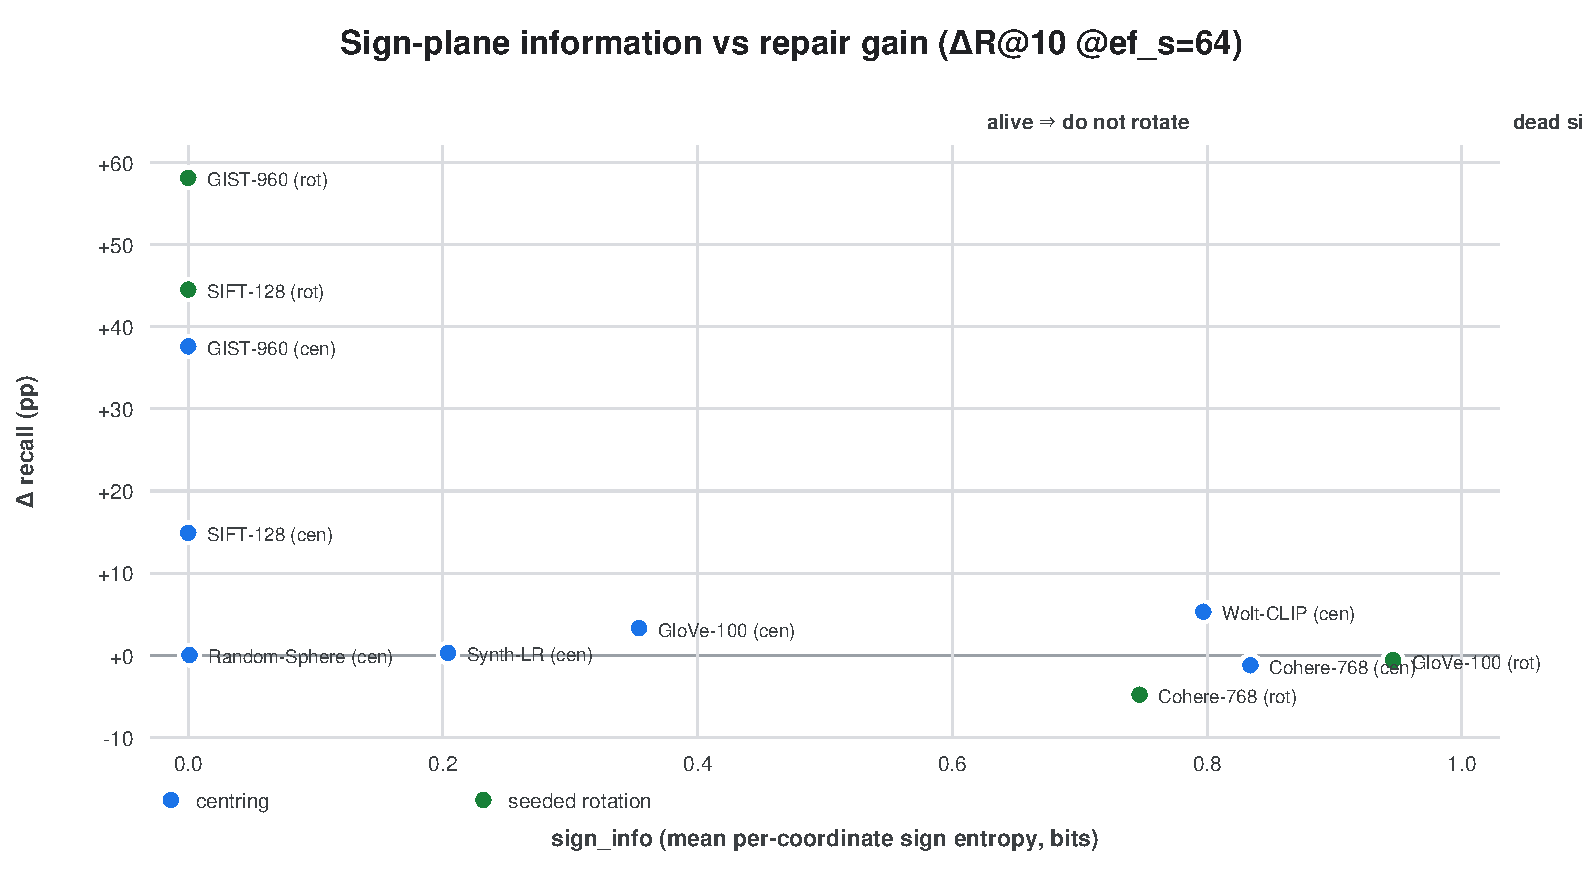
\includegraphics[keepaspectratio,alt={Figure 3.
Sign-plane information (sign\_info) vs repair gain $\Delta$R@10 at ef\_s = 64
for the centring and seeded-rotation arms. The statistic separates the
two regimes: sign\_info = 0.000 $\Rightarrow$ rotate (+44\ldots+58 pp), alive ($\geq$
0.6) $\Rightarrow$ do not rotate (Cohere $-$4.8 pp). The isotropic control sits at
+0.03 pp.}]{figures/fig3-signinfo-gain.pdf}}
\caption{\textbf{Figure 3.} Sign-plane information
(\protect\texttt{sign\_info}) vs repair gain $\Delta$R@10 at
\protect\texttt{ef\_s\ =\ 64} for the centring and seeded-rotation arms.
The statistic separates the two regimes:
\protect\texttt{sign\_info\ =\ 0.000} $\Rightarrow$ rotate (+44\ldots+58 pp), alive
($\geq$ 0.6) $\Rightarrow$ do not rotate (Cohere $-$4.8 pp). The isotropic control sits at
+0.03 pp.}
\end{figure}

\subsection{8.4 The competitor map: what the repair does and does not
buy}\label{the-competitor-map-what-the-repair-does-and-does-not-buy}

Same task on both sides (the centred task's own GT; competitor curves
rebuilt on the centred data), so the verdict is machine-independent.
``Pipeline upper'' = centring + weighted navigation.

{\def\LTcaptype{none} % do not increment counter
\begin{longtable}[]{@{}
  >{\raggedright\arraybackslash}p{(\linewidth - 10\tabcolsep) * \real{0.1667}}
  >{\raggedright\arraybackslash}p{(\linewidth - 10\tabcolsep) * \real{0.1667}}
  >{\raggedright\arraybackslash}p{(\linewidth - 10\tabcolsep) * \real{0.1667}}
  >{\raggedright\arraybackslash}p{(\linewidth - 10\tabcolsep) * \real{0.1667}}
  >{\raggedright\arraybackslash}p{(\linewidth - 10\tabcolsep) * \real{0.1667}}
  >{\raggedright\arraybackslash}p{(\linewidth - 10\tabcolsep) * \real{0.1667}}@{}}
\toprule\noalign{}
\begin{minipage}[b]{\linewidth}\raggedright
Tier
\end{minipage} & \begin{minipage}[b]{\linewidth}\raggedright
Arm
\end{minipage} & \begin{minipage}[b]{\linewidth}\raggedright
Before: QuIVer upper / HNSW \texttt{ef=64}
\end{minipage} & \begin{minipage}[b]{\linewidth}\raggedright
After: pipeline upper (@QPS)
\end{minipage} & \begin{minipage}[b]{\linewidth}\raggedright
After: competitor (best point)
\end{minipage} & \begin{minipage}[b]{\linewidth}\raggedright
Verdict
\end{minipage} \\
\midrule\noalign{}
\endhead
\bottomrule\noalign{}
\endlastfoot
collapse & GIST-960 & 4.38 \% / 84.11 \% @5,417 & \textbf{82.77 \%}
@4,717 & 84.85 \% @6,734 & dominated $\rightarrow$ \textbf{dominated} (gap 79.7 $\rightarrow$
\textbf{2.1 pp}) \\
collapse & SIFT-128 & 47.21 \% / 97.46 \% @45,118 & \textbf{92.47 \%}
@15,629 & 97.06 \% @50,547 (centred curve) & dominated $\rightarrow$
\textbf{dominated} (49.9 $\rightarrow$ \textbf{4.6 pp}; baseline also 3.2$\times$ faster at
that recall) \\
collapse & Random-Sphere & 6.46 \% / \textbf{1.40 \%} (HNSW also
collapses) & \textbf{17.78 \%} @1,867 & 17.43 \% @285 (ef=1024) &
\textbf{parity-or-better: 6.3--7.9$\times$ faster at matched recall} \\
usable & GloVe-100 & 71.69 \% / 82.05 \% @36,047 & \textbf{93.32 \%}
@11,675 & 93.45 \% @10,893 (ef=256) & dominated $\rightarrow$ \textbf{parity
($\approx$1.07$\times$)} \\
usable & Synthetic-LR & 92.52 \% / \emph{not measured on the original
task} & \textbf{97.05 \%} @2,638 & USearch 97.45 \% @375; FAISS-HNSW
97.90 \% @342 & after: \textbf{QuIVer \textasciitilde7.0--8.5$\times$ faster at
matched recall} (no ``before'' verdict available) \\
moderate & Wolt-CLIP-512 & 86.81 \% / 87.86 \% @19,606 & \textbf{89.05
\%} @9,356 & 87.88 \% @20,849 (centred curve) & dominated $\rightarrow$
\textbf{curves intersect} ($\leq$87.9 \% baseline 1.1--1.3$\times$ faster; $\geq$89 \%
QuIVer \textbf{2.3--3.9$\times$} faster) \\
competitive & Cohere-768 & 99.78 \% / 96.30 \% @9,514 (HNSW's best point
99.84 \% @741 $\Rightarrow$ $\approx$4.6$\times$ at \textasciitilde99.8 \%) & \textbf{99.89 \%}
@4,037 & 99.93 \% @1,435 (99.79 \% @2,544) & win $\rightarrow$ \textbf{win,
narrower: $\approx$2.7--3.4$\times$} at matched recall \\
\end{longtable}
}

\textbf{The honest sentence this table requires}: \emph{a smaller gap is
not availability.} GIST and SIFT move from ``hopeless'' to ``within 2--5
pp'' --- but at that recall the baseline is also faster. The arms where
the verdict actually changes are GloVe (\textbf{dominated $\rightarrow$ parity}) and
Wolt-CLIP (\textbf{dominated $\rightarrow$ intersecting}); on Random-Sphere and
Synthetic-LR QuIVer's pipeline is the faster index at matched recall,
but in the first case \emph{no} graph index is usable and in the second
the ``before'' verdict was never measured. On the competitive tier the
win survives centring but narrows ($\approx$4.6$\times$ $\rightarrow$ $\approx$2.7--3.4$\times$), because centring
helps HNSW as well: its centred curve is faster at the same recall
(99.79 \% @2,544 vs 99.84 \% @741 uncentred).

\subsection{8.5 What this repair is not}\label{what-this-repair-is-not}

\begin{itemize}
\tightlist
\item
  It does not change the similarity function's \emph{meaning} (L3) --- a
  deployer must accept centered-cosine.
\item
  It does not help index-agnostic collapse (Random-Sphere,
  Gaussian-960): +0.03 pp.
\item
  It does not touch the competitive tier's victory, and it does not
  create one where none existed.
\item
  It adds no new theory: the mechanism is the paper's own Finding 1, and
  centring is known post-processing. The contribution is the
  \textbf{triage rule} (\texttt{sign\_info}) + the
  \textbf{quantification} + the two-arm delivery path.
\end{itemize}

\subsection{8.6 A second repair, and on the collapse tier a better one:
a seeded
rotation}\label{a-second-repair-and-on-the-collapse-tier-a-better-one-a-seeded-rotation}

Centring has the defect we disclosed up front (L3): it \textbf{changes
the similarity function}. There is a classical alternative that does not
--- a random orthogonal transform. For unit vectors
\texttt{cos(Qa,\ Qb)\ =\ cos(a,b)}, so \textbf{the task is provably
unchanged} (we verify it: the rotated task's GT overlaps the original's
by \textbf{99.87--100 \%}), while the \emph{code} is recomputed in a
basis where the sign plane is alive. We generate \texttt{Q} by
QR-factorising a Gaussian matrix from a \textbf{fixed seed}, so it costs
\textbf{zero storage} (dim + seed suffice) and no training --- it is the
same device RaBitQ uses.

\textbf{Collapse tier: rotation beats centring, and keeps the task.}

{\def\LTcaptype{none} % do not increment counter
\begin{longtable}[]{@{}
  >{\raggedright\arraybackslash}p{(\linewidth - 12\tabcolsep) * \real{0.1429}}
  >{\raggedright\arraybackslash}p{(\linewidth - 12\tabcolsep) * \real{0.1429}}
  >{\raggedright\arraybackslash}p{(\linewidth - 12\tabcolsep) * \real{0.1429}}
  >{\raggedright\arraybackslash}p{(\linewidth - 12\tabcolsep) * \real{0.1429}}
  >{\raggedright\arraybackslash}p{(\linewidth - 12\tabcolsep) * \real{0.1429}}
  >{\raggedright\arraybackslash}p{(\linewidth - 12\tabcolsep) * \real{0.1429}}
  >{\raggedright\arraybackslash}p{(\linewidth - 12\tabcolsep) * \real{0.1429}}@{}}
\toprule\noalign{}
\begin{minipage}[b]{\linewidth}\raggedright
Dataset
\end{minipage} & \begin{minipage}[b]{\linewidth}\raggedright
original @ef=64
\end{minipage} & \begin{minipage}[b]{\linewidth}\raggedright
centred @ef=64
\end{minipage} & \begin{minipage}[b]{\linewidth}\raggedright
\textbf{rotated @ef=64}
\end{minipage} & \begin{minipage}[b]{\linewidth}\raggedright
original @1024
\end{minipage} & \begin{minipage}[b]{\linewidth}\raggedright
centred @1024
\end{minipage} & \begin{minipage}[b]{\linewidth}\raggedright
\textbf{rotated @1024}
\end{minipage} \\
\midrule\noalign{}
\endhead
\bottomrule\noalign{}
\endlastfoot
GIST-960 & 2.10 \% & 39.74 \% & \textbf{60.22 \%} (+58.1 pp) & 4.38 \% &
79.44 \% & \textbf{88.99 \%} \\
SIFT-128 & 15.77 \% & 30.64 \% & \textbf{60.24 \%} (+44.5 pp) & 47.23 \%
& 85.21 \% & \textbf{95.74 \%} \\
\end{longtable}
}

Graph construction also gets \textbf{2--6$\times$ faster} (GIST 290.4 s $\rightarrow$ 47.2
s; Cohere 202.4 s $\rightarrow$ 31.5 s), and the sign statistic moves from
\texttt{sign\_info\ =\ 0.000} to 0.507/0.759.

\textbf{\ldots but it is not a universal repair.} Rotation mixes
coordinates: it revives the sign plane and \emph{flattens} the magnitude
plane. So it is a pure win exactly where the magnitude plane was a
\emph{harmful} signal, and a loss where both planes carried information:

{\def\LTcaptype{none} % do not increment counter
\begin{longtable}[]{@{}
  >{\raggedright\arraybackslash}p{(\linewidth - 8\tabcolsep) * \real{0.2000}}
  >{\raggedright\arraybackslash}p{(\linewidth - 8\tabcolsep) * \real{0.2000}}
  >{\raggedright\arraybackslash}p{(\linewidth - 8\tabcolsep) * \real{0.2000}}
  >{\raggedright\arraybackslash}p{(\linewidth - 8\tabcolsep) * \real{0.2000}}
  >{\raggedright\arraybackslash}p{(\linewidth - 8\tabcolsep) * \real{0.2000}}@{}}
\toprule\noalign{}
\begin{minipage}[b]{\linewidth}\raggedright
Tier
\end{minipage} & \begin{minipage}[b]{\linewidth}\raggedright
Dataset
\end{minipage} & \begin{minipage}[b]{\linewidth}\raggedright
\texttt{sign\_info} before $\rightarrow$ after
\end{minipage} & \begin{minipage}[b]{\linewidth}\raggedright
$\Delta$ @ef=64
\end{minipage} & \begin{minipage}[b]{\linewidth}\raggedright
reading
\end{minipage} \\
\midrule\noalign{}
\endhead
\bottomrule\noalign{}
\endlastfoot
collapse & GIST-960 & 0.000 $\rightarrow$ 0.507 & \textbf{+58.1 pp} & sign plane
dead, magnitude plane harmful $\Rightarrow$ rotating is pure gain \\
collapse & SIFT-128 & 0.000 $\rightarrow$ 0.759 & \textbf{+44.5 pp} & same \\
usable & GloVe-100 & 0.946 $\rightarrow$ 0.938 & $-$0.6 pp alone, \textbf{+21.8 pp}
with the weighted navigation & magnitude plane useful $\Rightarrow$ needs §8.3's nav
metric to pay off \\
competitive & Cohere-768 & 0.747 $\rightarrow$ 0.572 & \textbf{$-$4.8 pp} & both
planes useful $\Rightarrow$ rotation is a net loss \\
\end{longtable}
}

$\Rightarrow$ The decision rule stays \texttt{sign\_info}: \textbf{0.000 $\Rightarrow$ rotate}
(better than centring \emph{and} task-preserving); \textbf{alive $\Rightarrow$ do
not rotate} (Cohere's $-$4.8 pp is the empirical warning).

\textbf{Competitor consequence} (no re-measurement needed: the task is
unchanged, so the §5 curves still apply):

{\def\LTcaptype{none} % do not increment counter
\begin{longtable}[]{@{}
  >{\raggedright\arraybackslash}p{(\linewidth - 8\tabcolsep) * \real{0.2000}}
  >{\raggedright\arraybackslash}p{(\linewidth - 8\tabcolsep) * \real{0.2000}}
  >{\raggedright\arraybackslash}p{(\linewidth - 8\tabcolsep) * \real{0.2000}}
  >{\raggedright\arraybackslash}p{(\linewidth - 8\tabcolsep) * \real{0.2000}}
  >{\raggedright\arraybackslash}p{(\linewidth - 8\tabcolsep) * \real{0.2000}}@{}}
\toprule\noalign{}
\begin{minipage}[b]{\linewidth}\raggedright
Dataset
\end{minipage} & \begin{minipage}[b]{\linewidth}\raggedright
matched point
\end{minipage} & \begin{minipage}[b]{\linewidth}\raggedright
rotated QuIVer
\end{minipage} & \begin{minipage}[b]{\linewidth}\raggedright
strongest competitor
\end{minipage} & \begin{minipage}[b]{\linewidth}\raggedright
verdict
\end{minipage} \\
\midrule\noalign{}
\endhead
\bottomrule\noalign{}
\endlastfoot
\textbf{GIST-960} & \textasciitilde84.4 \% & \textbf{84.41 \% @7,148} &
hnswlib 84.11 \% @5,417 & \textbf{QuIVer 1.32$\times$ faster} \\
& \textasciitilde89.0 \% & 88.99 \% @3,609 & IVF-Flat 88.36 \% @765 &
4.7$\times$ vs IVF; $\approx$parity vs HNSW (interpolated) \\
& \textbf{60--84 \% band} & 42,261 $\rightarrow$ 7,148 QPS & \textbf{no operating
point} (hnswlib's lowest \texttt{ef=64} already gives 84.11 \%) & in
that band QuIVer is the only option measured here \\
SIFT-128 & \textasciitilde95.7 \% & 95.74 \% @17,536 & hnswlib
\textbf{97.46 \% @45,118} & \textbf{Still dominated} (gap 49.9 $\rightarrow$
\textbf{1.7 pp}) \\
\end{longtable}
}

$\Rightarrow$ \textbf{GIST-960 moves from ``strictly dominated (79.7 pp gap)'' to
``faster at both ends of the usable band, and the only option in the
60--84 \% band''.} SIFT stays dominated --- HNSW is simply excellent
there --- but the gap shrinks from \textasciitilde50 pp to \textbf{1.7
pp}, and no task definition is harmed in either case.

\begin{figure}
\centering
\pandocbounded{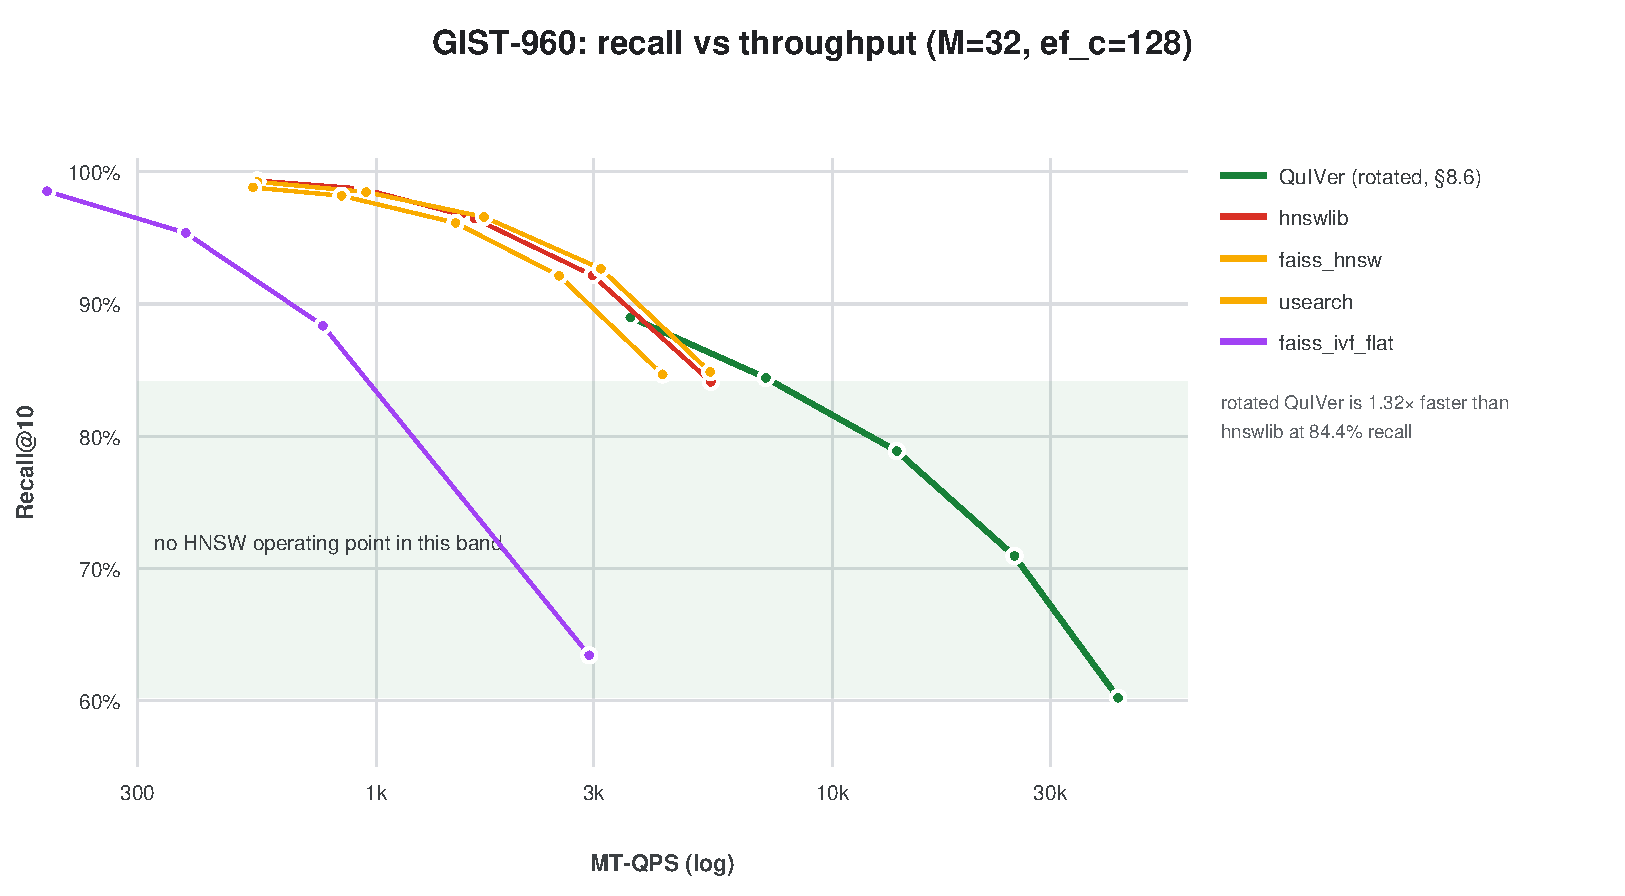
\includegraphics[keepaspectratio,alt={Figure 2. GIST-960
under the rotated code: recall vs throughput against the competitor
curves (same task, same machine, 32 threads). In the shaded band
60.2--84.1 \% there is no HNSW operating point --- the baseline's lowest
setting already yields 84.11 \%; at $\approx$ 84.4 \% the rotated index is 1.32$\times$
faster than hnswlib.}]{figures/fig2-gist960-curves.pdf}}
\caption{\textbf{Figure 2.} GIST-960 under the rotated code: recall vs
throughput against the competitor curves (same task, same machine, 32
threads). In the shaded band 60.2--84.1 \% there is no HNSW operating
point --- the baseline's \emph{lowest} setting already yields 84.11 \%;
at $\approx$ 84.4 \% the rotated index is 1.32$\times$ faster than hnswlib.}
\end{figure}

\textbf{One more thing rotation buys us.} Because the two navigation
metrics of §8.3 are decided by the \emph{same} code-only probe, we can
now pick the navigation metric \emph{predictively} instead of by
\texttt{sign\_info}: use the weighted navigation iff
\texttt{probe\_ef(weighted)\ \textgreater{}\ probe\_ef(cheap)}. Across
the ten arms where we have both the probe pair and an A/B measurement,
this rule gets the \textbf{sign right in 9 cases}; the single miss
(\texttt{wolt\_clip}) has $-$0.5 pp probe difference and +0.9 pp measured
difference, i.e.~both inside the noise floor. It also fixes the one
place where the \texttt{sign\_info\ $\geq$\ 0.75} heuristic fails
(\texttt{sift128r}: \texttt{sign\_info\ =\ 0.759} would predict a gain,
the measurement is \textbf{$-$10.2 pp}).

\textbf{Deployment form: the rotation as a code-side switch.} Until now
the rotation was \emph{data-side} --- it rewrites
\texttt{train}/\texttt{test}, so the GT and the f32 re-ranking stage
move with it. Because \texttt{cos(Qa,Qb)\ =\ cos(a,b)}, the same repair
can ship as a switch that touches nothing else, and we implemented it
(\texttt{TRIVIUM\_SIGN\_ROTATE=\textless{}seed\textgreater{}}, §11.1;
default off $\Rightarrow$ bit-identical when unset):

{\def\LTcaptype{none} % do not increment counter
\begin{longtable}[]{@{}
  >{\raggedright\arraybackslash}p{(\linewidth - 8\tabcolsep) * \real{0.2000}}
  >{\raggedright\arraybackslash}p{(\linewidth - 8\tabcolsep) * \real{0.2000}}
  >{\raggedright\arraybackslash}p{(\linewidth - 8\tabcolsep) * \real{0.2000}}
  >{\raggedright\arraybackslash}p{(\linewidth - 8\tabcolsep) * \real{0.2000}}
  >{\raggedright\arraybackslash}p{(\linewidth - 8\tabcolsep) * \real{0.2000}}@{}}
\toprule\noalign{}
\begin{minipage}[b]{\linewidth}\raggedright
Dataset (original files, original GT)
\end{minipage} & \begin{minipage}[b]{\linewidth}\raggedright
off @ef=64
\end{minipage} & \begin{minipage}[b]{\linewidth}\raggedright
\textbf{on @ef=64}
\end{minipage} & \begin{minipage}[b]{\linewidth}\raggedright
off $\rightarrow$ on @1024
\end{minipage} & \begin{minipage}[b]{\linewidth}\raggedright
data-side rotation, for reference
\end{minipage} \\
\midrule\noalign{}
\endhead
\bottomrule\noalign{}
\endlastfoot
SIFT-128 & 15.77 \% & \textbf{62.66 \%} @141,403 & 47.23 \% $\rightarrow$
\textbf{95.94 \%} & 60.24 \% / 95.74 \% \\
GIST-960 & 2.10 \% & \textbf{61.76 \%} @23,148 & 4.38 \% $\rightarrow$ \textbf{90.66
\%} & 60.22 \% / 88.99 \% \\
\end{longtable}
}

The engine generates its own \texttt{Q} from a seed PRNG (no
linear-algebra dependency, zero storage) --- a \emph{different} matrix
from the Python side's --- and the numbers agree within run-to-run
noise, so the gain comes from the rotation itself, not from one lucky
basis. This is also the only one of our two repairs a deployer can adopt
without touching the data contract: centring changes the similarity
function (L3), rotation cannot. With \textbf{both} switches on
(\texttt{TRIVIUM\_SIGN\_ROTATE} + \texttt{TRIVIUM\_NAV\_WEIGHTED}) the
engine-side path also reproduces the data-side \texttt{rc} arm of §8.7
on \texttt{gist960c}: \textbf{80.12 \% @ef=64 / 97.13 \% @ef=1024},
against 80.17 \% / 97.53 \% data-side --- the two-step repair survives
in the switch form.

\textbf{Implementation trap worth reporting upstream.} The engine has
\textbf{two} vector$\rightarrow$code paths (\texttt{Bq2Signature::from\_vector} and
\texttt{Bq2Store::push\_from\_vector}). Rotating only the first leaves
the stored codes unrotated and SIFT-128 reads \textbf{0.01 \%} at
\texttt{ef=64} --- worse than doing nothing. All numbers above are from
the build where both paths share one transform (152 library tests pass).

\subsection{8.7 Is BQ-native still the right choice? The quantizer arm,
and what the repair costs in
memory}\label{is-bq-native-still-the-right-choice-the-quantizer-arm-and-what-the-repair-costs-in-memory}

The repair only matters if the repaired index is competitive in its
\emph{own} market --- and that market is not only graph indexes: the
paper's baseline list contains four quantizer pipelines. §5.6 gives the
verdicts; here is what they mean for the deployment choice, with the
memory term attached:

{\def\LTcaptype{none} % do not increment counter
\begin{longtable}[]{@{}
  >{\raggedright\arraybackslash}p{(\linewidth - 6\tabcolsep) * \real{0.2500}}
  >{\raggedright\arraybackslash}p{(\linewidth - 6\tabcolsep) * \real{0.2500}}
  >{\raggedright\arraybackslash}p{(\linewidth - 6\tabcolsep) * \real{0.2500}}
  >{\raggedright\arraybackslash}p{(\linewidth - 6\tabcolsep) * \real{0.2500}}@{}}
\toprule\noalign{}
\begin{minipage}[b]{\linewidth}\raggedright
Task
\end{minipage} & \begin{minipage}[b]{\linewidth}\raggedright
QuIVer, best repair
\end{minipage} & \begin{minipage}[b]{\linewidth}\raggedright
OPQ+IVF-PQ+Refine
\end{minipage} & \begin{minipage}[b]{\linewidth}\raggedright
Who wins
\end{minipage} \\
\midrule\noalign{}
\endhead
\bottomrule\noalign{}
\endlastfoot
Cohere-1M (competitive) & \textbf{99.78 \% @ 8,684} & 99.82 \% @ 2,330 &
QuIVer \textbf{3.7$\times$} at $\geq$ 99.0 \% recall (11$\times$ at $\geq$ 99.5 \%) \\
GIST-960, centred task & 82.77 \% (centred) $\rightarrow$ \textbf{88.99 \%}
(rotated) & \textbf{98.99 \% @ 3,242} & PQ, on accuracy \\
GIST-960, both repairs (\texttt{rc}, weighted nav) & \textbf{97.53 \% @
4,005} & 98.99 \% @ 3,242 & $\approx$parity: 1.5 pp for \textbf{4.7$\times$ less
memory} \\
SIFT-128, centred task & 84.57 \% (centred) $\rightarrow$ \textbf{95.74 \%}
(rotated) & \textbf{99.94 \% @ 2,151} & PQ, on accuracy (and HNSW
reaches 99.90 \%) \\
Wolt-CLIP-1M, centred task & 89.05 \% @ 9,788 & 89.66 \% @ 3,809 &
tie-bound (96.1 \% exact-scan ceiling) $\approx$parity \\
GloVe-100, centred task & 93.32 \% @ 11,675 & 96.61 \% @ 4,990 & split:
PQ accuracy, QuIVer QPS \\
\texttt{coco\_nomic} & 0.21 \% (0.70 \% rotated) & \textbf{98.42 \% @
7,771} & PQ, decisively \\
\end{longtable}
}

Memory triangle (1 M $\times$ 768, §11.3a):

{\def\LTcaptype{none} % do not increment counter
\begin{longtable}[]{@{}
  >{\raggedright\arraybackslash}p{(\linewidth - 4\tabcolsep) * \real{0.3333}}
  >{\raggedright\arraybackslash}p{(\linewidth - 4\tabcolsep) * \real{0.3333}}
  >{\raggedright\arraybackslash}p{(\linewidth - 4\tabcolsep) * \real{0.3333}}@{}}
\toprule\noalign{}
\begin{minipage}[b]{\linewidth}\raggedright
Index
\end{minipage} & \begin{minipage}[b]{\linewidth}\raggedright
resident bytes
\end{minipage} & \begin{minipage}[b]{\linewidth}\raggedright
recall reached
\end{minipage} \\
\midrule\noalign{}
\endhead
\bottomrule\noalign{}
\endlastfoot
bare IVF-PQ (no re-ranking) & \textbf{92 MB} & \textasciitilde62.6 \% \\
OPQ+IVF-PQ+Refine & $\approx$ 92 MB + 3,072 MB f32 copy $\approx$ \textbf{3.16 GiB} &
99.8 \% \\
hnswlib / FAISS-HNSW & 3.19 GiB / 3.19 GiB & 99.8 \% \\
\textbf{QuIVer (BQ-native), with both repairs} & \textbf{675 MiB} &
88.99 \% $\rightarrow$ \textbf{97.53 \%} \\
\end{longtable}
}

The honest reading: on collapse-tier data a PQ pipeline is \emph{more
accurate} than our best repair, and what our repair buys is not a win
but the same recall band at \textbf{4.7$\times$ less memory} --- a different
point on the curve, not a free lunch. On the competitive tier ($\geq$ 88 \%
recall) the BQ-native index wins outright and the memory advantage
becomes a bonus rather than the whole argument.

\section{9. Discussion}\label{discussion}

\subsection{9.1 The decision a deployer actually
faces}\label{the-decision-a-deployer-actually-faces}

Combining §5--§8 into one table --- every quantity is computable
\textbf{before} building an index, in seconds:

{\def\LTcaptype{none} % do not increment counter
\begin{longtable}[]{@{}
  >{\raggedright\arraybackslash}p{(\linewidth - 8\tabcolsep) * \real{0.2000}}
  >{\raggedright\arraybackslash}p{(\linewidth - 8\tabcolsep) * \real{0.2000}}
  >{\raggedright\arraybackslash}p{(\linewidth - 8\tabcolsep) * \real{0.2000}}
  >{\raggedright\arraybackslash}p{(\linewidth - 8\tabcolsep) * \real{0.2000}}
  >{\raggedright\arraybackslash}p{(\linewidth - 8\tabcolsep) * \real{0.2000}}@{}}
\toprule\noalign{}
\begin{minipage}[b]{\linewidth}\raggedright
\texttt{sign\_info}
\end{minipage} & \begin{minipage}[b]{\linewidth}\raggedright
\texttt{$\|$$\mu$$\|$} (headroom)
\end{minipage} & \begin{minipage}[b]{\linewidth}\raggedright
\texttt{probe\_ef} (min of both metrics)
\end{minipage} & \begin{minipage}[b]{\linewidth}\raggedright
what to do
\end{minipage} & \begin{minipage}[b]{\linewidth}\raggedright
expected outcome
\end{minipage} \\
\midrule\noalign{}
\endhead
\bottomrule\noalign{}
\endlastfoot
\textbf{= 0.000} (sign plane dead) & any & --- & \textbf{rotate (§8.6)}
--- task-preserving \emph{and} stronger; centre only if rotation is not
an option & GIST 2.10$\rightarrow$\textbf{60.22 \%}, SIFT 15.77$\rightarrow$\textbf{60.24 \%}
@ef=64 (centring: 39.74 / 30.64); GIST becomes \textbf{1.3$\times$ faster than
HNSW} at 84 \% recall \\
\textbf{$\geq$ 0.6}, \texttt{$\|$$\mu$$\|$\ $\geq$\ 0.3}, headroom \textgreater{} 5 pp &
large & $\geq$ 50 \% & centre as a cheap option & small-to-moderate gain
(+0.3\ldots+5.3 pp), never harmful in our 6-dataset set \\
\textbf{$\geq$ 0.6} but headroom $\leq$ 5 pp & large & $\geq$ 50 \% & \textbf{do not
bother} & Cohere: $-$1.2 pp (neutral) --- the tier is already at 95 \% \\
any & any & \textbf{\textless{} 50 \%} & \textbf{use a float32 index} &
the code cannot rank; the fault is not fixable by translation \\
\texttt{sign\_info} \textbf{= 1.000} but recall $\ll$ 50 \% &
\textasciitilde0 & \textless{} 50 \% & \textbf{do not build any graph
index on this task} & index-agnostic collapse (Random-Sphere,
Gaussian-960): HNSW also collapses (1.40 \%) \\
\end{longtable}
}

And one row the gate deliberately does \textbf{not} cover, because it
needs a competitor curve:

measured recall $\geq$ \textasciitilde88 \% on a competitive embedding
\textbar{} --- \textbar{} --- \textbar{} \textbf{QuIVer is the right
index}: 4.6--5.0$\times$ at matched recall vs the best HNSW \textbar{} the only
tier where the paper's index actually wins (§5) \textbar{}

\subsection{9.2 Translation or rotation? The
head-to-head}\label{translation-or-rotation-the-head-to-head}

Both revive the sign plane; they differ in what \emph{else} they change.
We ran the comparison (§8.6, seeded random rotation, zero storage, no
training):

{\def\LTcaptype{none} % do not increment counter
\begin{longtable}[]{@{}
  >{\raggedright\arraybackslash}p{(\linewidth - 6\tabcolsep) * \real{0.2500}}
  >{\raggedright\arraybackslash}p{(\linewidth - 6\tabcolsep) * \real{0.2500}}
  >{\raggedright\arraybackslash}p{(\linewidth - 6\tabcolsep) * \real{0.2500}}
  >{\raggedright\arraybackslash}p{(\linewidth - 6\tabcolsep) * \real{0.2500}}@{}}
\toprule\noalign{}
\begin{minipage}[b]{\linewidth}\raggedright
tier
\end{minipage} & \begin{minipage}[b]{\linewidth}\raggedright
centring
\end{minipage} & \begin{minipage}[b]{\linewidth}\raggedright
rotation
\end{minipage} & \begin{minipage}[b]{\linewidth}\raggedright
reading
\end{minipage} \\
\midrule\noalign{}
\endhead
\bottomrule\noalign{}
\endlastfoot
collapse (GIST / SIFT) & +37.6 / +14.9 pp @ef=64, but it
\textbf{replaces the task} (centred-cosine) & \textbf{+58.1 / +44.5 pp},
GT untouched (99.87--100 \% overlap) & \textbf{rotation wins} ---
stronger \emph{and} it changes nothing but the code \\
usable (GloVe) & +3.3 pp alone; ceiling \textbf{93.32 \%} with weighted
navigation & $-$0.6 pp alone; \textbf{88.45 \%} with weighted navigation
(54.06 \% @ef=64) & centring is better at the ceiling, rotation is
better at low \texttt{ef}; a wash in practice \\
competitive (Cohere) & $-$1.2 pp (neutral) & \textbf{$-$4.8 pp} & centring,
or leave it alone \\
\end{longtable}
}

So the ordering is not ``one dominates'': \textbf{for a dead sign plane,
rotate}; \textbf{for a live sign plane, do not rotate}. Both choices are
made by the same free statistic, so a deployer does not have to guess.
What remains open is the \emph{learned}-transform direction (L12): we
tested one seeded \textbf{random} rotation, not OPQ-style learned ones,
so 60.22 \% / 60.24 \% should be read as a \textbf{lower bound} on what
a transform-side repair can do.

\begin{figure}
\centering
\pandocbounded{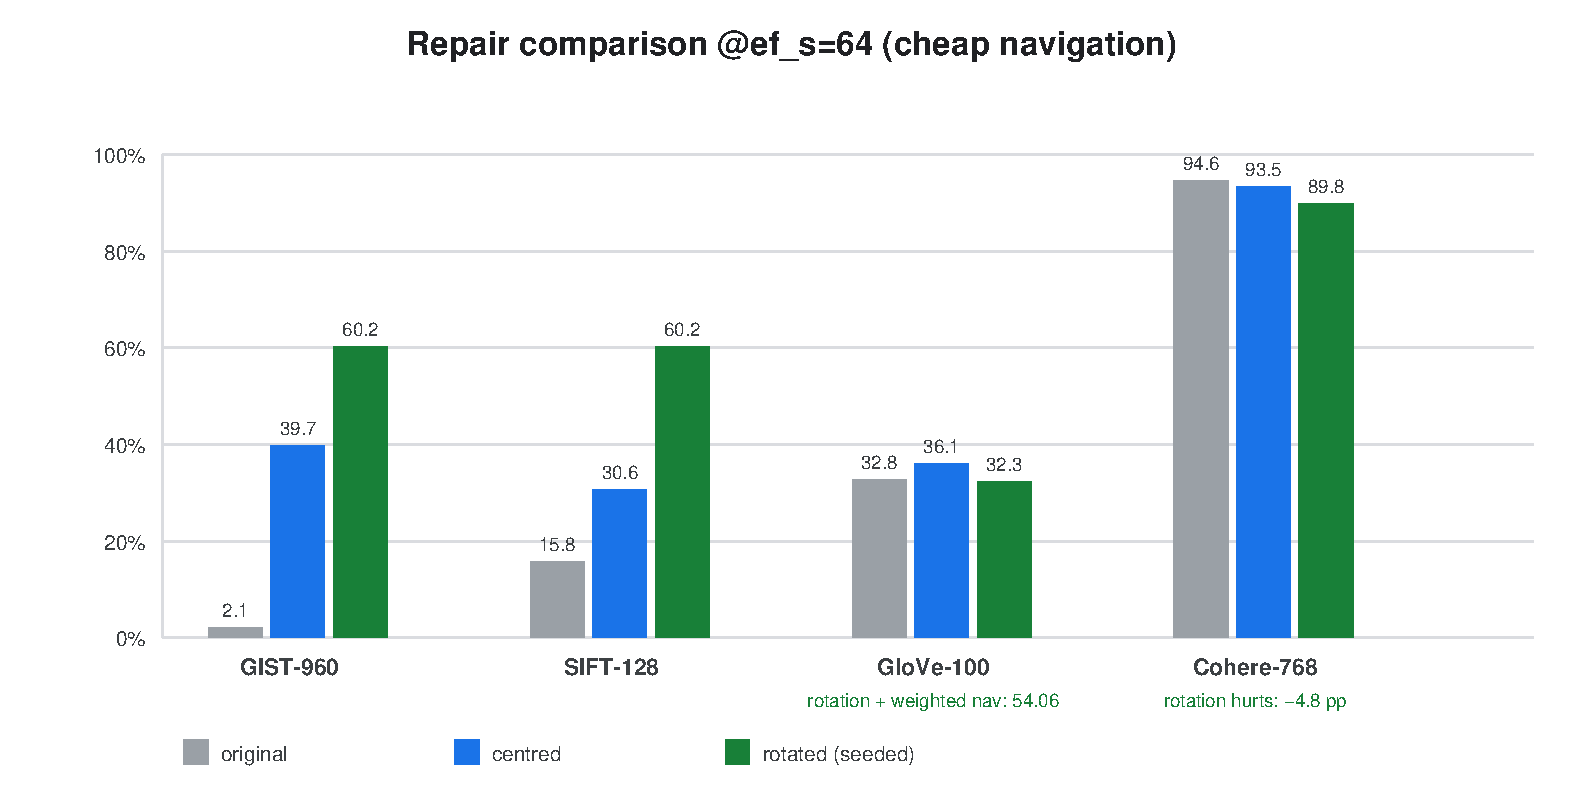
\includegraphics[keepaspectratio,alt={Figure 1. Repair
comparison at ef\_s = 64 (cheap navigation): original, centred and
seeded-rotated R@10 for four tier representatives. Rotation is a pure
gain only where the sign plane is dead (GIST-960 +58.1 pp, SIFT-128
+44.5 pp) and a loss on Cohere ($-$4.8 pp); centring is neutral-to-small
elsewhere.}]{figures/fig1-repair-bars.pdf}}
\caption{\textbf{Figure 1.} Repair comparison at
\protect\texttt{ef\_s\ =\ 64} (cheap navigation): original, centred and
seeded-rotated R@10 for four tier representatives. Rotation is a pure
gain only where the sign plane is dead (GIST-960 +58.1 pp, SIFT-128
+44.5 pp) and a loss on Cohere ($-$4.8 pp); centring is neutral-to-small
elsewhere.}
\end{figure}

\subsection{9.3 What this says about the published applicability
claim}\label{what-this-says-about-the-published-applicability-claim}

The paper's four tiers are an \textbf{applicability} gradient (a
description of achieved recall) and are read by practitioners as a
\textbf{competitiveness} gradient. Our competitor map (§8.4) shows the
two differ: before repair, three of the four tiers with competitor data
were dominated by HNSW; after repair, one becomes parity and one becomes
a genuine intersection --- but the only tier with a clear win remains
the competitive one. The practical statement we would put in a
deployment guide is therefore narrower than the paper's:

\begin{quote}
Use a BQ-native graph \textbf{when the embedding is competitive-tier ($\geq$
\textasciitilde88 \% recall) and you need memory/QPS}; on collapse-tier
data, first check \texttt{sign\_info} --- if it is 0.000, centre it,
knowing that this buys 2--5 pp of absolute recall but usually \emph{not}
the win.
\end{quote}

\subsection{9.4 A methodological note we owe the
reader}\label{a-methodological-note-we-owe-the-reader}

Both the paper's probe and our gate end up in the same place:
\textbf{there is no single scalar that predicts recall}. Our two
attempts to build one failed (§7.4), and the two strongest correlates we
found (graph fidelity, \texttt{sign\_info}) each have a counterexample
that forbids a monotone formula. The deliverable is therefore a
\textbf{triage rule plus a necessary condition}, with its abstention
made explicit --- which is, we suspect, the honest form of this kind of
result, and the reason we report the failures alongside the wins.

\subsection{9.5 Does the boundary appear outside the paper's twelve
datasets?
(VIBE)}\label{does-the-boundary-appear-outside-the-papers-twelve-datasets-vibe}

Table 11 is built from twelve datasets. We ran seven modern embedding
benchmarks that the paper never evaluates (VIBE,
\texttt{vector-index-bench/vibe}; 282 K -- 3.9 M vectors, 768-d) to ask
whether our triage rule extrapolates. It does --- and the extrapolation
is uncomfortable for the published claim:

{\def\LTcaptype{none} % do not increment counter
\begin{longtable}[]{@{}
  >{\raggedright\arraybackslash}p{(\linewidth - 10\tabcolsep) * \real{0.1667}}
  >{\raggedright\arraybackslash}p{(\linewidth - 10\tabcolsep) * \real{0.1667}}
  >{\raggedright\arraybackslash}p{(\linewidth - 10\tabcolsep) * \real{0.1667}}
  >{\raggedright\arraybackslash}p{(\linewidth - 10\tabcolsep) * \real{0.1667}}
  >{\raggedright\arraybackslash}p{(\linewidth - 10\tabcolsep) * \real{0.1667}}
  >{\raggedright\arraybackslash}p{(\linewidth - 10\tabcolsep) * \real{0.1667}}@{}}
\toprule\noalign{}
\begin{minipage}[b]{\linewidth}\raggedright
VIBE row
\end{minipage} & \begin{minipage}[b]{\linewidth}\raggedright
n $\times$ d
\end{minipage} & \begin{minipage}[b]{\linewidth}\raggedright
\texttt{sign\_info}
\end{minipage} & \begin{minipage}[b]{\linewidth}\raggedright
\texttt{probe\_ef} (min metric)
\end{minipage} & \begin{minipage}[b]{\linewidth}\raggedright
QuIVer @ ef=64 $\rightarrow$ @1024
\end{minipage} & \begin{minipage}[b]{\linewidth}\raggedright
hnswlib @ ef=64
\end{minipage} \\
\midrule\noalign{}
\endhead
\bottomrule\noalign{}
\endlastfoot
\texttt{coco\_nomic} & 282 K $\times$ 768 & 0.382 & \textbf{0.6 \%} $\Rightarrow$ ``use
float32'' & \textbf{0.21 \% $\rightarrow$ 3.59 \%} & \textbf{86.23 \%} @17,053 \\
\texttt{ccnews\_nomic} & 495 K $\times$ 768 & 0.690 & 99.0 \% $\Rightarrow$ ``usable'' &
25.65 \% $\rightarrow$ \textbf{99.64 \%} & (not measured) \\
\end{longtable}
}

Two readings:

\begin{itemize}
\tightlist
\item
  \textbf{\texttt{coco\_nomic} is a catastrophe of a kind the paper's
  table cannot contain} --- a modern, widely-used embedding benchmark on
  which the shipped index returns \textbf{0.21 \%} R@10 while plain HNSW
  returns 86 \% on the same task, with an exact scan at 100 \% (neither
  the GT nor the task is at fault). Our gate catches it before any index
  is built (\texttt{probe\_ef} = 0.6 \%), and \textbf{neither of our
  repairs rescues it} (rotation: 0.21 $\rightarrow$ 0.70 \%): this is failure type
  (iii) of §6.4, where the honest advice is ``change the code'' (PQ:
  98.42 \%).
\item
  \textbf{The probe estimates a ceiling, not a latency.}
  \texttt{ccnews\_nomic} probes at 99.0 \% while delivering 25.65 \% at
  \texttt{ef=64}; its 99.64 \% appears only at \texttt{ef\_s=1024}. So
  ``usable'' must never be read as ``fast at your operating point'' ---
  the §5 caveat restated in the one place where the two could be
  conflated.
\end{itemize}

Scope of this subsection: VIBE rows are an \textbf{extension}, not a
reproduction (they are not in Table 11), and two of the seven rows were
measured with the gate plus a single real-index sweep; the remaining
five rows are reported with their \texttt{sign\_info}/\texttt{probe}
verdicts only (§11.3).

\section{10. Limitations}\label{limitations}

All of the following are stated in the body text, not hidden in an
appendix.

\subsection{10.1 Platform and protocol}\label{platform-and-protocol}

{\def\LTcaptype{none} % do not increment counter
\begin{longtable}[]{@{}
  >{\raggedright\arraybackslash}p{(\linewidth - 4\tabcolsep) * \real{0.3333}}
  >{\raggedright\arraybackslash}p{(\linewidth - 4\tabcolsep) * \real{0.3333}}
  >{\raggedright\arraybackslash}p{(\linewidth - 4\tabcolsep) * \real{0.3333}}@{}}
\toprule\noalign{}
\begin{minipage}[b]{\linewidth}\raggedright
\#
\end{minipage} & \begin{minipage}[b]{\linewidth}\raggedright
Limitation
\end{minipage} & \begin{minipage}[b]{\linewidth}\raggedright
Mitigation / why the conclusion survives
\end{minipage} \\
\midrule\noalign{}
\endhead
\bottomrule\noalign{}
\endlastfoot
\textbf{L1} & \textbf{Single machine, no AVX-512} (Intel i9-14900K;
\texttt{Avx512F\ =\ false}) --- the VPOPCNTDQ path QuIVer is designed
around is never exercised & Recall-level conclusions are
machine-independent. For speed we report the same-recall ratio, and note
that our \textbf{absolute MT-QPS is already 1.1--2.4$\times$ the paper's} (32
vs 16 threads), i.e.~we are \emph{not} measuring on a weakened platform.
We do not assert the direction in which the ratio would move on Zen4. \\
\textbf{L2} & \textbf{Metric deviation}: the published SIFT/GIST rows
are \emph{Euclidean}, while the repository's \texttt{prepare\_all.py}
normalises and recomputes GT by cosine, so our SIFT/GIST rows are cosine
tasks & Disclosed in §4.2; our numbers are comparable to the paper's
\emph{pipeline}, not to the public Euclidean leaderboards. All our
\emph{comparisons} put both arms on the same task, so the deviation
cancels. \\
\textbf{L3} & \textbf{Centring changes the similarity function}: every
``after'' number in §8.2--§8.4 is Recall@10 on the \emph{centred-cosine}
task, not an improvement on the original task & Stated at the head of
§8. Centring is also known post-processing (all-but-the-top family); we
claim triage + quantification, not novelty of the transform.
\textbf{§8.6 covers this caveat by reporting a task-preserving
alternative (seeded rotation), which on the collapse tier is both
stronger and leaves the GT untouched (99.87--100 \% overlap).} \\
\textbf{L4} & The separability column (\textasciitilde5 \% calibre
uncertainty from \texttt{cos\_std}) appears in the gate's development
tables & It is \textbf{not} used as a criterion in the final chain
(§7.3), only reported for completeness. \\
\textbf{L16} & \textbf{GT / metric alignment must be verified per
dataset, not assumed.} For Cohere the shipped ground truth is cosine
while the on-disk f32 files are raw ($\|$x$\|$ $\approx$ 13.8), so any arm that does
not re-normalise is silently scored against a different objective ---
this \emph{inverted} our own first same-family measurement before it was
diagnosed (§5.6b). The shipped check
(\texttt{gt\_metric\_consistency\_probe.py}) now makes normalisation a
verified precondition for every arm. & \\
\end{longtable}
}

\subsection{10.2 The reproduction has one unresolved row, one tie
floor}\label{the-reproduction-has-one-unresolved-row-one-tie-floor}

{\def\LTcaptype{none} % do not increment counter
\begin{longtable}[]{@{}
  >{\raggedright\arraybackslash}p{(\linewidth - 2\tabcolsep) * \real{0.5000}}
  >{\raggedright\arraybackslash}p{(\linewidth - 2\tabcolsep) * \real{0.5000}}@{}}
\toprule\noalign{}
\begin{minipage}[b]{\linewidth}\raggedright
\#
\end{minipage} & \begin{minipage}[b]{\linewidth}\raggedright
Limitation
\end{minipage} \\
\midrule\noalign{}
\endhead
\bottomrule\noalign{}
\endlastfoot
\textbf{L5} & \textbf{RedCaps-1M (77.08 \% vs 78.41 \%)}: the sampling
protocol (which 1 M slice; whether self-matches are excluded) is
unstated in the paper, and the four plausible readings span \textbf{7.4
pp}. We report the reading that is closest to the paper and flag the row
as partially reproduced. \\
\textbf{L6} & \textbf{Wolt-CLIP has a tie floor}: \texttt{faiss\_exact}
itself scores \textbf{90.09 \%} on this 1 M set, so the achievable
ceiling is \textasciitilde90 \%. The ``intersecting curves'' verdict in
§8.4 is therefore partly caused by ties, and this dataset's recall must
not be compared with other datasets' (Cohere / GloVe / SIFT have
\texttt{faiss\_exact} $\geq$ 99.9 \%). The centred variant used from §8.4 on
is likewise tie-limited: exact scan \textbf{96.1 \%} (§5.6a, §8.7). \\
\end{longtable}
}

\subsection{10.3 Experimental scope}\label{experimental-scope}

{\def\LTcaptype{none} % do not increment counter
\begin{longtable}[]{@{}
  >{\raggedright\arraybackslash}p{(\linewidth - 2\tabcolsep) * \real{0.5000}}
  >{\raggedright\arraybackslash}p{(\linewidth - 2\tabcolsep) * \real{0.5000}}@{}}
\toprule\noalign{}
\begin{minipage}[b]{\linewidth}\raggedright
\#
\end{minipage} & \begin{minipage}[b]{\linewidth}\raggedright
Limitation
\end{minipage} \\
\midrule\noalign{}
\endhead
\bottomrule\noalign{}
\endlastfoot
\textbf{L7} & \textbf{Single M (32), single \texttt{ef\_c} (128), single
build per arm.} Graph construction is concurrent and not
bit-reproducible; we measured the spread over \textbf{3 independent
builds $\times$ 5 representatives} (§3.5): \textbf{$\leq$ 0.25 pp} at \texttt{ef=64}
(per dataset: GIST 0.22 / SIFT 0.25 / GloVe 0.10 / Wolt 0.19 / Cohere
0.16). Any graph-structure quantity (fidelity, CSR-derived) is a
256-node single-sample estimate. \\
\textbf{L8} & \textbf{Our own two single-scalar predictors failed}
(§7.4). Reported as negative results; the delivered chain is triage + a
necessary condition, and explicitly abstains on competitiveness. \\
\textbf{L9} & \st{Memory footprint not reproduced} $\rightarrow$ \textbf{reproduced
(§11.3a)}: the paper's ``$\approx$4.7$\times$ less hot memory / \textless{} 1.3 GB per
1 M'' is confirmed at \textbf{1:4.73} and \textbf{675 MiB per 1 M $\times$ 768}
(hnswlib 3,193 MiB, FAISS-HNSW 3,189 MiB, IVF-Flat 2,949 MiB). Remaining
caveat: we measured the \textbf{index bytes}, not peak RSS, and not the
per-query hot-set growth. \\
\textbf{L10} & \textbf{MSMARCO-5M scalability (Table 12) is out of
scope} --- a 5 M-scale run is beyond this study's budget, so the paper's
scaling claim is neither confirmed nor contradicted here. \\
\textbf{L11} & \textbf{The multi-signal (TSNG) path was not A/B-tested
under the navigation-metric switch} (§8.3 covers the main path only). \\
\textbf{L12} & \textbf{Only a \emph{random} (seeded) orthogonal
transform was tested} (§8.6): we did not compare against learned
rotations (OPQ-style) or other orthogonal transforms, and we do not
claim rotation is optimal --- only that it dominates centring on the
collapse tier (60.22 \% vs 39.74 \% on GIST-960) while preserving the
task. The row is therefore a \emph{lower} bound on what a transform-side
repair can achieve. \\
\textbf{L13} & \textbf{Two baselines named by the paper could not be
built on this machine} (§5.3's DiskANN-Rust and VSAG): DiskANN-Rust
fails in \texttt{openblas-src} for want of a C/C++/BLAS toolchain
(\texttt{vcpkg}, \texttt{cmake}, \texttt{cl}, \texttt{gcc} all absent),
and the \texttt{pyvsag} wheel installed here is a Linux/\texttt{cp310}
build. These two arms are therefore \textbf{missing, not measured as
slow} --- a claim we deliberately do not make. Our competitor map covers
hnswlib, FAISS-HNSW, USearch, IVF-Flat, \texttt{faiss\_exact}, and (for
quantizers) OPQ+IVF-PQ+Refine. \\
\textbf{L14} & \textbf{The quantizer comparison is one configuration
family.} Our PQ arm uses OPQ + IVF-PQ + exact f32 re-ranking; our RaBitQ
arm is same-family (\texttt{IndexIVFRaBitQ} + f32 refine), with a
normalised FastScan+SQ8 spot check used only as a recall-side
consistency signal --- neither reproduces the paper's exact
implementation, and the paper's DiskANN PQ+FP and SSD arms are not run.
The same-family arm also required a protocol correction (Cohere's GT is
cosine while its files are raw): its raw-vector numbers are retracted,
and the corrected pair is in §5.6(b). Tier-jump PQ numbers were measured
on six cells; they establish that PQ does \emph{not} collapse on them,
not that PQ dominates everywhere. \\
\textbf{L15} & \textbf{The VIBE rows are an extension, not a
reproduction} (§9.5): they are not part of the paper's Table 11, and of
the seven VIBE benchmarks only two (\texttt{coco\_nomic},
\texttt{ccnews\_nomic}) received a full gate + real-index sweep; the
other five carry \texttt{sign\_info}/probe verdicts and their two
navigation arms. \\
\end{longtable}
}

\subsection{10.4 Statistical conventions used
throughout}\label{statistical-conventions-used-throughout}

\begin{itemize}
\tightlist
\item
  Recall values are single-run unless labelled; the spread measured over
  \textbf{3 independent builds} is $\leq$ 0.25 pp, so differences below
  \textasciitilde0.3 pp are not interpreted.
\item
  Probe values (§7) always come with their sample size and the
  query-subset spread (4--7 pp); a single-run probe value is never
  quoted alone. The shipped table uses \textbf{K = 5 disjoint query
  subsets} (artifact field \texttt{probe\_k}); re-running it at K = 3
  changes no verdict and no value by more than 1.7 pp (§7.3).
\item
  With the navigation switch \textbf{off}, frozen recall values
  reproduce within $\leq$ 0.17 pp (Cohere 97.52 / GIST-960 2.79 / GloVe-100
  45.60), which is the regression guard for all \texttt{src/} work in
  §8.3.
\item
  Competitor QPS numbers are quoted with the thread count that produced
  them; the competitor map is \textbf{thread-aligned at 32} (§11.3),
  because QPS at 16 vs 32 threads differs by up to \textasciitilde2$\times$.
\end{itemize}

\section{11. Artifacts and
Reproduction}\label{artifacts-and-reproduction}

\begin{quote}
Every number in §4--§9 was produced by the code below on the machine
described in §4.2, with \texttt{RUSTFLAGS="-C\ target-cpu=native"} and
\texttt{-\/-features\ ablation}.
\end{quote}

\subsection{11.1 Index-side harness (Rust bench, no library changes
except the Sec. 8.3
switch)}\label{index-side-harness-rust-bench-no-library-changes-except-the-sec.-8.3-switch}

{\def\LTcaptype{none} % do not increment counter
\begin{longtable}[]{@{}
  >{\raggedright\arraybackslash}p{(\linewidth - 2\tabcolsep) * \real{0.5000}}
  >{\raggedright\arraybackslash}p{(\linewidth - 2\tabcolsep) * \real{0.5000}}@{}}
\toprule\noalign{}
\begin{minipage}[b]{\linewidth}\raggedright
Artifact
\end{minipage} & \begin{minipage}[b]{\linewidth}\raggedright
Purpose
\end{minipage} \\
\midrule\noalign{}
\endhead
\bottomrule\noalign{}
\endlastfoot
\texttt{benches/bench\_t2\_b2\_partitioned.rs} & the main arm:
partitioned BQ search, single-arm mode (recall + MT-QPS + build time),
frozen-value guard (\texttt{T2\_FROZEN\_RECALL}) \\
\texttt{benches/bench\_t2\_build\_recon.rs} & exports the L0 CSR for
graph-fidelity measurement (§6.3) \\
\texttt{src/index/bq.rs}, \texttt{src/index/quiver.rs},
\texttt{src/tsng.rs} & the only library change in this work:
\texttt{TRIVIUM\_NAV\_WEIGHTED} (default \textbf{off} $\Rightarrow$ behaviour
bit-identical; regression guard as above). Shipped as
\texttt{patches/f1-nav-weighted.patch} for upstream review \\
\end{longtable}
}

\subsection{\texorpdfstring{11.2 Data preparation and analysis scripts
(Python; \texttt{src/}
untouched)}{11.2 Data preparation and analysis scripts (Python; src/ untouched)}}\label{data-preparation-and-analysis-scripts-python-src-untouched}

{\def\LTcaptype{none} % do not increment counter
\begin{longtable}[]{@{}
  >{\raggedright\arraybackslash}p{(\linewidth - 2\tabcolsep) * \real{0.5000}}
  >{\raggedright\arraybackslash}p{(\linewidth - 2\tabcolsep) * \real{0.5000}}@{}}
\toprule\noalign{}
\begin{minipage}[b]{\linewidth}\raggedright
Script
\end{minipage} & \begin{minipage}[b]{\linewidth}\raggedright
Produces
\end{minipage} \\
\midrule\noalign{}
\endhead
\bottomrule\noalign{}
\endlastfoot
\texttt{scripts/prepare\_all.py} & the 12 benchmarking datasets
(HF/ann-benchmarks sources), normalised + cosine GT \\
\texttt{scripts/research/gist960\_collapse\_prepare.py} & centred
variants of any dataset
(\texttt{-\/-center\ \textless{}prefix\textgreater{}:\textless{}dim\textgreater{}}),
with the \texttt{$\|$$\mu$$\|$\ $\leq$\ 1} guard of §8.1 \\
\texttt{scripts/research/bq2\_code\_ceiling.py} & the analytic code-only
ceiling; \texttt{verify\_identities()} asserts analytic == bitwise
against \texttt{src/index/bq.rs} \\
\texttt{scripts/research/deployability\_gate.py} & the 22-arm gate table
of §7.3 (\texttt{sign\_info}, \texttt{$\|$$\mu$$\|$}, \texttt{probe10},
\texttt{probe\_ef}, verdict) \\
\texttt{scripts/research/compat\_probe\_scaling.py} & sample-size /
query-subset sensitivity of the published probe (§7.2) \\
\texttt{scripts/research/graph\_neighbor\_quality.py} &
\texttt{L0\ $\cap$\ \{cos,\ weighted,\ cheap\}\_top64} (§6.3) \\
\texttt{scripts/research/baseline\_competitors.py} & hnswlib /
FAISS-HNSW / USearch / IVF-Flat / \texttt{faiss\_exact} curves on the
same task (§5, §8.4); \texttt{BL\_SKIP} can drop an arm \\
\texttt{scripts/research/ivf\_recall\_diagnostic.py} & the
wrapper/parameter audit of §5.6(b): does \texttt{nprobe} reach the
wrapped base, what does \texttt{k\_factor} actually do, where does the
exact arm saturate \\
\texttt{scripts/research/gt\_metric\_consistency\_probe.py} & the
GT/vector metric check of §5.6(b): which exact search reproduces the
shipped ground truth \\
\texttt{scripts/research/faiss\_refine\_mechanics\_probe.py} & the
synthetic mechanics probe of §5.6(b): refine metric, default
\texttt{k\_factor}, monotonicity on a self-consistent task \\
\end{longtable}
}

\subsection{11.3 Where each table comes
from}\label{where-each-table-comes-from}

{\def\LTcaptype{none} % do not increment counter
\begin{longtable}[]{@{}
  >{\raggedright\arraybackslash}p{(\linewidth - 2\tabcolsep) * \real{0.5000}}
  >{\raggedright\arraybackslash}p{(\linewidth - 2\tabcolsep) * \real{0.5000}}@{}}
\toprule\noalign{}
\begin{minipage}[b]{\linewidth}\raggedright
Paper table
\end{minipage} & \begin{minipage}[b]{\linewidth}\raggedright
Source of record
\end{minipage} \\
\midrule\noalign{}
\endhead
\bottomrule\noalign{}
\endlastfoot
§4.3 (12 rows) & \texttt{results/t2/*/} per-dataset bench logs; frozen
values in \texttt{docs/research/HANDOFF.md} \\
§5.3 (tier $\times$ competitor map) &
\texttt{results/baseline/competitors\_*.json} \\
§6.3 (graph fidelity) &
\texttt{results/t2/gist960\_collapse/graph\_quality\_*.json} (9 files;
fields \texttt{overlap\_cos\_pct} / \texttt{overlap\_w\_pct} /
\texttt{overlap\_c\_pct}) \\
§7.2--7.3 (gate + probe sensitivity) &
\texttt{results/t2/deployability\_gate.json},
\texttt{results/t2/p2\_probe\_scaling.json} \\
§8.2--8.3 (centre + navigation A/B) &
\texttt{results/t2/gist960\_collapse/*.json} \\
§8.4 (7-arm map) & \texttt{results/baseline/competitors\_*c.json} \\
§8.6 (rotation) & derived \texttt{*r\_*.f32/i32} sets (\texttt{gist960r}
/ \texttt{sift128r} / \texttt{glove100r} / \texttt{coherer}, produced by
\texttt{gist960\_collapse\_prepare.py\ -\/-rotate}, with the
GT-invariance check) + \texttt{.tmp/p4a\_*.log}; diagnosis in
\texttt{docs/research/p4a-rotation-vs-centering.md} \\
§10-L9 (memory) & \texttt{results/t2/memory\_footprint\_cohere.json}
(script \texttt{scripts/research/memory\_index\_footprint.py}; log
\texttt{.tmp/p4b\_memory\_cohere.log}) \\
\end{longtable}
}

\subsubsection{11.3a Memory footprint (1 M x 768, M =
32)}\label{a-memory-footprint-1-m-x-768-m-32}

{\def\LTcaptype{none} % do not increment counter
\begin{longtable}[]{@{}
  >{\raggedright\arraybackslash}p{(\linewidth - 6\tabcolsep) * \real{0.2500}}
  >{\raggedright\arraybackslash}p{(\linewidth - 6\tabcolsep) * \real{0.2500}}
  >{\raggedright\arraybackslash}p{(\linewidth - 6\tabcolsep) * \real{0.2500}}
  >{\raggedright\arraybackslash}p{(\linewidth - 6\tabcolsep) * \real{0.2500}}@{}}
\toprule\noalign{}
\begin{minipage}[b]{\linewidth}\raggedright
Implementation
\end{minipage} & \begin{minipage}[b]{\linewidth}\raggedright
index bytes
\end{minipage} & \begin{minipage}[b]{\linewidth}\raggedright
B/vector
\end{minipage} & \begin{minipage}[b]{\linewidth}\raggedright
vs QuIVer
\end{minipage} \\
\midrule\noalign{}
\endhead
\bottomrule\noalign{}
\endlastfoot
\textbf{QuIVer (2-bit BQ)} & \textbf{675 MiB} & 707.8 & 1.00$\times$ (paper
claims \textless{} 1.3 GB / 1 M: confirmed) \\
hnswlib & 3,193 MiB & 3,348.2 & \textbf{4.73$\times$} (paper claims 4.7$\times$:
confirmed) \\
FAISS-HNSW & 3,189 MiB & 3,344.1 & 4.72$\times$ \\
FAISS IVF-Flat (nlist $\approx$ 4 k) & 2,949 MiB & 3,092.3 & 4.37$\times$ \\
\textbf{Bare IVF-PQ} (nlist = 1,024, m = 96, \textbf{no rerank}) &
\textbf{92 MiB} & 96.5 & 0.14$\times$ --- but its recall caps at \textbf{62.6
\%} \\
\textbf{OPQ+IVF-PQ+Refine} (PQ codes + f32 rerank copy) & $\approx$ \textbf{3.16
GiB} (92 MiB + 3,072 MiB) & 3,312 & 4.8$\times$ --- needed to reach 99.8 \% \\
\end{longtable}
}

$\Rightarrow$ The quantizer comparison sharpens the memory claim: \textbf{on PQ,
cheap memory and high recall are mutually exclusive} (bare PQ is 92 MiB
at 62.6 \%; the refined pipeline is 3.16 GiB at 99.8 \%). Only the
BQ-native index gives 675 MiB \textbf{and} 99.8 \% at the same time
(§5.6 / §11.3b).

Measured as index bytes (bench-reported \texttt{Hot} for QuIVer;
\texttt{save\_index} size for hnswlib; \texttt{serialize\_index} length
for FAISS), not peak RSS. The 2-bit code accounts for \textasciitilde183
MiB of QuIVer's 675 MiB (\texttt{0.25\ B/dim\ $\times$\ 768\ $\times$\ 1\ M}); the
rest is graph + bookkeeping, and the per-dimension increment across our
128/256/512/768-dim arms (522 $\rightarrow$ 553 $\rightarrow$ 614 $\rightarrow$ 675 MiB, $\approx$ 0.25 B/dim)
matches 2 bits per dimension exactly. The repair arms (\texttt{c} /
\texttt{r}) keep the same footprint (720 MiB on \texttt{gist960} and
\texttt{gist960r} alike).

\subsection{11.4 One-command reproduction of the central
claim}\label{one-command-reproduction-of-the-central-claim}

\begin{Shaded}
\begin{Highlighting}[]
\CommentTok{\# 1. build}
\VariableTok{RUSTFLAGS}\OperatorTok{=}\StringTok{"{-}C target{-}cpu=native"} \ExtensionTok{cargo}\NormalTok{ build }\AttributeTok{{-}{-}release} \AttributeTok{{-}{-}features}\NormalTok{ ablation}

\CommentTok{\# 2. dataset + centred variant (GIST{-}960 as the example)}
\ExtensionTok{python}\NormalTok{ scripts/prepare\_all.py gist960}
\ExtensionTok{python}\NormalTok{ scripts/research/gist960\_collapse\_prepare.py }\AttributeTok{{-}{-}center}\NormalTok{ gist960:960}

\CommentTok{\# 3. before / after (single arm, includes the frozen{-}value guard)}
\VariableTok{T2\_PREFIX}\OperatorTok{=}\NormalTok{gist960  }\VariableTok{T2\_DIM}\OperatorTok{=}\NormalTok{960 }\VariableTok{T2\_FROZEN\_RECALL}\OperatorTok{=}\NormalTok{2.79 }\ExtensionTok{cargo}\NormalTok{ bench }\AttributeTok{{-}{-}features}\NormalTok{ ablation }\AttributeTok{{-}{-}bench}\NormalTok{ bench\_t2\_b2\_partitioned}
\VariableTok{T2\_PREFIX}\OperatorTok{=}\NormalTok{gist960c }\VariableTok{T2\_DIM}\OperatorTok{=}\NormalTok{960 }\ExtensionTok{cargo}\NormalTok{ bench }\AttributeTok{{-}{-}features}\NormalTok{ ablation }\AttributeTok{{-}{-}bench}\NormalTok{ bench\_t2\_b2\_partitioned}

\CommentTok{\# 4. the gate (seconds, no index)}
\ExtensionTok{python}\NormalTok{ scripts/research/deployability\_gate.py}
\end{Highlighting}
\end{Shaded}

Expected: GIST-960 \texttt{R@10\ @ef=64} $\approx$ \textbf{2.1 \%} before and $\approx$
\textbf{39.7 \%} after centring (the paper's row is 2.01 \%); the gate
reports \texttt{sign\_info\ =\ 0.000} for \texttt{gist960} and 0.981 for
\texttt{gist960c}.

\subsection{11.5 Upstream material (parallel
track)}\label{upstream-material-parallel-track}

{\def\LTcaptype{none} % do not increment counter
\begin{longtable}[]{@{}
  >{\raggedright\arraybackslash}p{(\linewidth - 2\tabcolsep) * \real{0.5000}}
  >{\raggedright\arraybackslash}p{(\linewidth - 2\tabcolsep) * \real{0.5000}}@{}}
\toprule\noalign{}
\begin{minipage}[b]{\linewidth}\raggedright
Artifact
\end{minipage} & \begin{minipage}[b]{\linewidth}\raggedright
Content
\end{minipage} \\
\midrule\noalign{}
\endhead
\bottomrule\noalign{}
\endlastfoot
\texttt{docs/research/upstream-issues.md} & the full audit of the
upstream reports (Chinese), including the one we retracted ourselves \\
\texttt{docs/research/upstream-issue-draft.md} & the paste-ready
\textbf{English} version of those reports (five issues; not yet
filed) \\
\texttt{patches/f1-nav-weighted.patch} & the §8.3 switch as a reviewable
patch (default off) \\
\texttt{docs/research/*.md} & the full audit trail: every claim, its
evidence, and the conclusions we retracted (three of our own) \\
\end{longtable}
}

\subsection{11.6 Artifacts added after the first draft (second repair,
quantizer arm, external
validity)}\label{artifacts-added-after-the-first-draft-second-repair-quantizer-arm-external-validity}

All library changes remain \textbf{default-off and bit-identical when
unset}; \texttt{src/} now carries two such switches
(\texttt{TRIVIUM\_NAV\_WEIGHTED} from §8.3,
\texttt{TRIVIUM\_SIGN\_ROTATE} from §8.6), plus 2 new unit tests (152
library tests pass with both off and on).

{\def\LTcaptype{none} % do not increment counter
\begin{longtable}[]{@{}
  >{\raggedright\arraybackslash}p{(\linewidth - 6\tabcolsep) * \real{0.2500}}
  >{\raggedright\arraybackslash}p{(\linewidth - 6\tabcolsep) * \real{0.2500}}
  >{\raggedright\arraybackslash}p{(\linewidth - 6\tabcolsep) * \real{0.2500}}
  >{\raggedright\arraybackslash}p{(\linewidth - 6\tabcolsep) * \real{0.2500}}@{}}
\toprule\noalign{}
\begin{minipage}[b]{\linewidth}\raggedright
§
\end{minipage} & \begin{minipage}[b]{\linewidth}\raggedright
Claim
\end{minipage} & \begin{minipage}[b]{\linewidth}\raggedright
Script
\end{minipage} & \begin{minipage}[b]{\linewidth}\raggedright
Product
\end{minipage} \\
\midrule\noalign{}
\endhead
\bottomrule\noalign{}
\endlastfoot
8.6 (rotation, data side) & rotation preserves the task (GT overlap
99.87--100 \%) and beats centring on the collapse tier &
\texttt{scripts/research/gist960\_collapse\_prepare.py\ -\/-rotate/-\/-rotate-center}
& \texttt{*r\_train.f32} / \texttt{*rc\_train.f32} +
\texttt{.tmp/p4a\_*.log} \\
8.6 (rotation, engine side) & the same repair as one env var on the
original files/GT & \texttt{src/index/bq.rs}
(\texttt{TRIVIUM\_SIGN\_ROTATE}) + \texttt{bench\_t2\_b2\_partitioned} &
\texttt{.tmp/p5\_*.log} \\
5.6 / 8.7 (quantizers) & PQ does not collapse where the 2-bit code does
(six cells); QuIVer is 3.7$\times$ faster at $\geq$ 99 \% on Cohere &
\texttt{scripts/research/pq\_matched\_recall.py},
\texttt{benches/bench\_baselines.py} (mode A/B) &
\texttt{results/t2/pq\_matched\_recall\_\{cohere,sift128c,wolt\_clipc\}.json}
(from \texttt{.tmp/p7\_pq\_*.log}),
\texttt{results/baseline/competitors\_cohere.json} \\
5.6(b) (RaBitQ same-family + the normalisation trap) & the raw-vector
inversion, the parameter audit (\texttt{k\_factor}), the GT-metric
check, and the corrected (normalised) pair &
\texttt{scripts/research/bench\_rabitq\_refine.py}
(\texttt{RA\_CONTROL}, \texttt{RA\_NORMALIZE}),
\texttt{ivf\_recall\_diagnostic.py},
\texttt{gt\_metric\_consistency\_probe.py},
\texttt{faiss\_refine\_mechanics\_probe.py} &
\texttt{results/t2/\{rabitq\_refine,ivfflat\_control\}\_cohere.json}
(raw-metric; kept as the trap record),
\texttt{\{rabitq\_refine,ivfflat\_control\}\_norm\_cohere.json} (of
record), \texttt{ivf\_recall\_diagnostic\_cohere.json},
\texttt{gt\_metric\_consistency\_cohere.json},
\texttt{faiss\_refine\_mechanics\_probe.json},
\texttt{rabitq\_refine\_gist960c.json} \\
6.4(ii) (second witness) & every competitor collapses on Gaussian-960
(hnswlib / FAISS-HNSW / USearch / IVF-Flat) &
\texttt{scripts/research/baseline\_competitors.py} (\texttt{BL\_SKIP}
optional) & \texttt{results/baseline/competitors\_gauss960.json} \\
8.6 (engine-side \texttt{rc}) & both switches reproduce the data-side
\texttt{rc} arm on \texttt{gist960c} (80.12 / 97.13) &
\texttt{bench\_t2\_b2\_partitioned} + \texttt{TRIVIUM\_SIGN\_ROTATE} +
\texttt{TRIVIUM\_NAV\_WEIGHTED} & \texttt{.tmp/p8\_10\_engine\_rc.log}
(retry product, after the queue's first attempt failed) \\
P8 queue & the ten-step unattended batch behind the rows above &
\texttt{scripts/research/p8\_queue.py},
\texttt{scripts/research/p8\_collect\_numbers.py} &
\texttt{results/t2/p8\_queue\_summary.json} + \texttt{.tmp/p8\_*.log}
(step-10 retry note: \texttt{docs/research/p8-queue-report.md} §4-D5) \\
6.5 (bit budget) & 2-bit allocation vs 4-bit ceiling on the four
collapse datasets & \texttt{scripts/research/bit\_budget\_probe.py} &
\texttt{results/t2/bit\_budget\_*.json} \\
7.3 (prospective validation) & nav-metric rule held out on 6 arms: 6/6 &
\texttt{scripts/research/nav\_rule\_validation.py} &
\texttt{results/t2/nav\_rule\_validation.json} \\
9.5 (external validity) & seven VIBE benchmarks; \texttt{coco\_nomic} is
a new catastrophe &
\texttt{scripts/research/download\_vibe\_parallel.py},
\texttt{scripts/research/convert\_hdf5\_to\_f32.py} &
\texttt{.tmp/p6\_vibe\_*.log} + gate rows in
\texttt{results/t2/deployability\_gate.json} \\
3.5 / 10.3 (noise floor) & 3 builds $\times$ 5 datasets $\Rightarrow$ spread $\leq$ 0.25 pp &
\texttt{bench\_t2\_b2\_partitioned} re-runs &
\texttt{.tmp/p7q\_*\_seed\{1,2,3\}.log},
\texttt{results/t2/p7\_stagec\_report.json} \\
7.3 (probe K = 5) & K = 3 $\rightarrow$ K = 5 changes no verdict, drift $\leq$ 1.7 pp &
\texttt{scripts/research/deployability\_gate.py} (K = 5),
\texttt{scripts/research/p7\_k5\_vs\_k3.py} &
\texttt{results/t2/deployability\_gate.json},
\texttt{results/t2/p7\_k5\_vs\_k3.json} \\
11.3a (memory) & QuIVer 675 MiB vs refined PQ $\approx$ 3.16 GiB vs hnswlib 3.19
GiB & \texttt{scripts/research/memory\_footprint.py} &
\texttt{results/t2/memory\_footprint\_cohere.json} \\
\end{longtable}
}

Reproducing §8.6's engine-side switch end to end:

\begin{Shaded}
\begin{Highlighting}[]
\VariableTok{TRIVIUM\_SIGN\_ROTATE}\OperatorTok{=}\NormalTok{20260923 }\VariableTok{T2\_PREFIX}\OperatorTok{=}\NormalTok{sift128 }\VariableTok{T2\_DIM}\OperatorTok{=}\NormalTok{128 }\DataTypeTok{\textbackslash{}}
  \ExtensionTok{cargo}\NormalTok{ bench }\AttributeTok{{-}{-}features}\NormalTok{ ablation }\AttributeTok{{-}{-}bench}\NormalTok{ bench\_t2\_b2\_partitioned   }\CommentTok{\# 15.77 \% {-}\textgreater{} 62.66 \% @ef=64}
\end{Highlighting}
\end{Shaded}

\section{12. References, Artifact Statement, and How to Assemble This
Draft}\label{references-artifact-statement-and-how-to-assemble-this-draft}

\begin{quote}
Every entry below was checked against its published version on
2026-10-09 (arXiv ids, venues and author lists verified against the
arXiv abstract pages). We list what we actually used, with the version
we used.
\end{quote}

\subsection{12.1 The object of study}\label{the-object-of-study}

\begin{enumerate}
\def\labelenumi{\arabic{enumi}.}
\tightlist
\item
  \textbf{QuIVer: Rethinking ANN Graph Topology via Training-Free Binary
  Quantization.} W. Xiao, Z. Wang, C. Li. arXiv:2605.02171 (2026),
  cs.DB. --- the paper evaluated and extended throughout §§4--7.
\item
  \textbf{README\_QUIVER.md} (shipped with the implementation). ---
  dataset preparation, benchmark drivers, and the step-by-step
  reproduction guide this work follows. §4.2's ``one protocol
  deviation'' is a deviation from \emph{this} document, not from the
  paper text.
\item
  Repository README (\texttt{README.md} / \texttt{README\_EN.md}) ---
  the published claims about hot/cold memory separation, the dimension
  guidance ($\leq$ 3072), and the TSNG research track. §5 and §11.3a check
  the memory claim; §10.3/L11 records that the TSNG path was not
  A/B-tested under our navigation switch.
\end{enumerate}

\subsection{12.2 Baseline implementations we measured
against}\label{baseline-implementations-we-measured-against}

{\def\LTcaptype{none} % do not increment counter
\begin{longtable}[]{@{}
  >{\raggedright\arraybackslash}p{(\linewidth - 4\tabcolsep) * \real{0.3333}}
  >{\raggedright\arraybackslash}p{(\linewidth - 4\tabcolsep) * \real{0.3333}}
  >{\raggedright\arraybackslash}p{(\linewidth - 4\tabcolsep) * \real{0.3333}}@{}}
\toprule\noalign{}
\begin{minipage}[b]{\linewidth}\raggedright
\#
\end{minipage} & \begin{minipage}[b]{\linewidth}\raggedright
Baseline
\end{minipage} & \begin{minipage}[b]{\linewidth}\raggedright
Reference / source
\end{minipage} \\
\midrule\noalign{}
\endhead
\bottomrule\noalign{}
\endlastfoot
4 & HNSW (algorithm) & Yu. A. Malkov, D. A. Yashunin. \emph{Efficient
and robust approximate nearest neighbor search using Hierarchical
Navigable Small World graphs.} IEEE TPAMI 42(4), 2020.
arXiv:1603.09320 \\
5 & hnswlib (implementation) & https://github.com/nmslib/hnswlib \\
6 & FAISS (library) & J. Johnson, M. Douze, H. Jégou.
\emph{Billion-scale similarity search with GPUs.} IEEE Trans. Big Data,
2019. arXiv:1702.08734; and M. Douze, A. Guzhva, C. Deng, J. Johnson, G.
Szilvasy, P.-E. Mazaré, M. Lomeli, L. Hosseini, H. Jégou. \emph{The
Faiss library.} arXiv:2401.08281 (2025) \\
7 & USearch (implementation) & https://github.com/unum-cloud/usearch \\
8 & Inverted-file index (IVF / IVF-Flat) & J. Sivic, A. Zisserman.
\emph{Video Google: a text retrieval approach to object matching in
videos.} ICCV 2003 \\
9 & Product quantization (PQ) & H. Jégou, M. Douze, C. Schmid.
\emph{Product quantization for nearest neighbor search.} IEEE TPAMI
33(1), 2011 \\
10 & Optimized PQ (OPQ) & T. Ge, K. He, Q. Ke, J. Sun. \emph{Optimized
product quantization for approximate nearest neighbor search.} CVPR
2013 \\
11 & RaBitQ & J. Gao, C. Long. \emph{RaBitQ: Quantizing high-dimensional
vectors with a theoretical error bound for approximate nearest neighbor
search.} SIGMOD 2024 (DOI 10.1145/3654970). arXiv:2405.12497 \\
12 & DiskANN / Vamana graph & S. Subramanya, et al.~\emph{DiskANN: Fast
accurate billion-point nearest neighbor search on a single node.}
NeurIPS 2019 \\
13 & FAISS \texttt{IndexIVFRaBitQ} / \texttt{IndexRefineFlat} /
\texttt{IndexPreTransform} & FAISS 1.15 API (the same-family RaBitQ arm
of §5.6(b), and the PQ arm of §5.6(a)) \\
\end{longtable}
}

\emph{Not measured, and why:} the paper's DiskANN-\textbf{Rust} and VSAG
arms (§10.3/L13) --- a C/C++/BLAS toolchain is absent on the evaluation
machine and the \texttt{pyvsag} wheel available there is a
Linux/build-mismatched artifact.

\subsection{12.3 Background and method
references}\label{background-and-method-references}

\begin{enumerate}
\def\labelenumi{\arabic{enumi}.}
\setcounter{enumi}{13}
\tightlist
\item
  J. Mu, P. Viswanath. \emph{All-but-the-Top: Simple and effective
  postprocessing for word representations.} ICLR 2018. arXiv:1702.01417
  --- the centring step of §8.1 is this post-processing, applied to the
  query and base vectors before quantization.
\item
  \textbf{VIBE: Vector Index Benchmark for Embeddings.} E. Jääsaari, V.
  Hyvönen, M. Ceccarello, T. Roos, M. Aumüller. arXiv:2505.17810 (2025);
  J. Data-centric ML Research (2026) ---
  https://github.com/vector-index-bench/vector-index-bench. The seven
  external benchmarks of §9.5.
\item
  Embedding models whose released vectors we use (Cohere-768,
  OpenAI-1536/3072, Nomic-768, Jina-768, DINOv2, MiniLM, BGE-M3,
  GloVe-100, Wolt-CLIP-512): cited via the dataset preparation scripts
  of (2) and (15), which name the model and revision for each row. We
  make no claim about the models themselves.
\end{enumerate}

\subsection{12.4 Artifact statement (what is ours, what is upstream, and
the
licence)}\label{artifact-statement-what-is-ours-what-is-upstream-and-the-licence}

The upstream project is licensed \textbf{Apache-2.0} (\texttt{LICENSE}).
This fork keeps that licence, and every change we made is confined to
the following, so a reader can separate our work from upstream's line by
line:

{\def\LTcaptype{none} % do not increment counter
\begin{longtable}[]{@{}
  >{\raggedright\arraybackslash}p{(\linewidth - 4\tabcolsep) * \real{0.3333}}
  >{\raggedright\arraybackslash}p{(\linewidth - 4\tabcolsep) * \real{0.3333}}
  >{\raggedright\arraybackslash}p{(\linewidth - 4\tabcolsep) * \real{0.3333}}@{}}
\toprule\noalign{}
\begin{minipage}[b]{\linewidth}\raggedright
Directory / file
\end{minipage} & \begin{minipage}[b]{\linewidth}\raggedright
Ours?
\end{minipage} & \begin{minipage}[b]{\linewidth}\raggedright
Content
\end{minipage} \\
\midrule\noalign{}
\endhead
\bottomrule\noalign{}
\endlastfoot
\texttt{Cargo.toml}, \texttt{src/**} (except two switches) & upstream &
the QuIVer implementation we evaluate \\
\texttt{src/index/bq.rs} & \textbf{ours, +2 switches} &
\texttt{TRIVIUM\_NAV\_WEIGHTED} (§8.3) and
\texttt{TRIVIUM\_SIGN\_ROTATE} (§8.6): both \textbf{default off and
bit-identical when unset}, shipped as reviewable patches in
\texttt{patches/}, plus 2 new unit tests \\
\texttt{benches/bench\_t2\_b2\_partitioned.rs} & upstream & the
index-side harness we drive via \texttt{T2\_*} environment variables (no
source change needed) \\
\texttt{benches/bench\_baselines.py} & upstream, \textbf{+env overrides}
& grids/thread counts made overridable so the quantizer arm can be run
at 32 threads (§10.4) \\
\texttt{scripts/research/**} & \textbf{ours} & index-free gate,
competitor maps, rotation/centring preparation, PQ \& RaBitQ arms,
bit-budget probe, memory footprint, multi-seed spread, all report
scripts \\
\texttt{docs/paper/**} & \textbf{ours} & this draft (§0--§12) \\
\texttt{docs/research/**} & \textbf{ours} & the audit trail: every claim
with its evidence, \textbf{including our own conclusions that were
retracted along the way} (most recently the raw-vector RaBitQ numbers,
§5.6b) \\
\texttt{results/**}, \texttt{.tmp/**} & \textbf{ours (generated)} &
products and logs. \texttt{results/**} is the citable store;
\texttt{.tmp/**} holds raw stdout and the execution queue \\
\end{longtable}
}

\textbf{Traceability.} Every number in this draft resolves to a file
under \texttt{results/**} or a log under \texttt{.tmp/**}, and §11.3 +
§11.6 give the table $\rightarrow$ artifact mapping. Statements without an artifact
are explicitly labelled as assumptions (e.g.~the RedCaps row, §4.4).

\textbf{Reproduction entry points.} §11.4 (the central claim, five
commands) and §11.6 (the second repair, the quantizer arm, the external
benchmarks). The full unattended batch that produced the last group of
numbers is \texttt{scripts/research/p8\_queue.py}, whose per-step log
and summary (\texttt{results/t2/p8\_queue\_summary.json}) are part of
the artifact.

\textbf{What is \emph{not} in the artifact.} The upstream paper's own
source or LaTeX; the VIBE and embedding-model downloads (public, large,
and pinned by their own repositories); and the two blocked baselines of
§10.3/L13.

\end{document}
